\setcounter{deso}{0}
\begin{name}
	{\tenchude}
	{TỔNG HỢP TRẮC NGHIỆM ABCD VÀ ĐÚNG SAI}
	{LỚP TOÁN THẦY PHÁT}
	{\lq\lq  It's not how much time you have, it's how you use it.\rq\rq}
\end{name}
\setcounter{ex}{0}
\begin{ex}%[0D0H2-4]%[Đề thi thử môn Toán TRƯỜNG THPT Hàm Rồng năm học 2025-2026]%[Dương Phạm - GVPB2 Đỗ Minh Vũ]
	Một lớp có $25$ học sinh nam và $15$ học sinh nữ. Chọn ngẫu nhiên $3$ học sinh của lớp lên bảng. Xác suất sao cho trong ba bạn được chọn có đúng hai học sinh nam và một học sinh nữ là
	\choice
	{$\dfrac{63}{1976}$}
	{$\dfrac{17}{25}$}
	{$\dfrac{75}{104}$}
	{\True $\dfrac{225}{494}$}
	\loigiai{
		Số phần tử của không gian mẫu $n(\Omega) = \mathrm{C}_{40}^3 = 9880$.\\
		Gọi $A$ là biến cố \lq\lq Trong ba bạn được chọn có đúng hai học sinh nam và một học sinh nữ\rq\rq.\\
		Số cách chọn $2$ học sinh nam từ $25$ học sinh nam là $\mathrm{C}_{25}^2$.\\
		Số cách chọn $1$ học sinh nữ từ $15$ học sinh nữ là $\mathrm{C}_{15}^1$.\\
		Suy ra $n(A) = \mathrm{C}_{25}^2 \cdot \mathrm{C}_{15}^1 = 4500$.\\
		Vậy $\mathrm{P}(A) = \dfrac{n(A)}{n(\Omega)} = \dfrac{4500}{9880} = \dfrac{225}{494}$.
	}
\end{ex}

\begin{ex}%[0D0H2-4]%[Dự án C đề thi thử TN Môn Toán NH25-26 - Dot 4 - Hồng Trường Sơn]%[THPT Mai Anh Tuấn - Thanh Hóa]%[GVPB - Lê Hữu Kiệt]
	Trong một lớp có $15$ học sinh nam và $10$ học sinh nữ. Giáo viên gọi $4$ học sinh lên bảng làm bài tập. Tính xác suất để $4$ học sinh lên bảng có nam và nữ.
	\choice
	{\True $\dfrac{443}{506}$}
	{$\dfrac{400}{501}$}
	{$\dfrac{443}{501}$}
	{$\dfrac{307}{506}$}
	\loigiai{
		Số phần tử của không gian mẫu là $n(\Omega)=\mathrm{C}_{25}^4=12\,650$.\\
		Gọi biến cố $A\colon$ \lq\lq$4$ học sinh được chọn có cả nam và nữ\rq\rq.\\
		Khi đó biến cố $\overline{A}\colon $ \lq\lq$4$ học sinh được chọn chỉ toàn nam hoặc nữ\rq\rq.\\
		Ta có $n\left(\overline{A}\right)=\mathrm{C}_{15}^4+\mathrm{C}_{10}^4=1\,575.$\\
		Suy ra $\mathrm{P}\left(\overline{A}\right)=\dfrac{n\left(\overline{A}\right)}{n(\Omega)}=\dfrac{1\,575}{12\,650}=\dfrac{63}{506}$.\\
		Vậy xác suất cần tìm là
		$$\mathrm{P}(A)=1-\mathrm{P}\left(\overline{A}\right)=1-\dfrac{63}{506}=\dfrac{443}{506}.$$
	}
\end{ex}

\begin{ex}%[0D0N2-2]%[Dự án đề thi thử NH25-26]%[THPT Chuyên Phan Bội Châu - Nghệ An]%[GVPB2 Khắc Thiên]
	Gieo một đồng xu cân đối đồng chất $3$ lần. Xác suất để cả $3$ lần xuất hiện mặt ngửa là
	\choice
	{$\dfrac{7}{8}$}
	{$\dfrac{1}{6}$}
	{\True $\dfrac{1}{8}$}
	{$\dfrac{1}{2}$}
	\loigiai{
		Vì các lần gieo độc lập với nhau và xác suất xuất hiện mặt ngửa ở mỗi lần là $\dfrac{1}{2}$.\\
		Do đó xác suất để cả $3$ lần đều xuất hiện mặt ngửa là $\mathrm{P}(A) = \dfrac{1}{2} \cdot \dfrac{1}{2} \cdot \dfrac{1}{2} = \dfrac{1}{8}$.
	}
\end{ex}

\begin{ex}%[0D6N4-2]%[Dự án đề thi thử NH25-26]%[THPT Chuyên Phan Bội Châu - Nghệ An]%[GVPB2 Khắc Thiên]
	Cho mẫu số liệu ghép nhóm có bảng tần số như sau:
	\begin{center}
		\begin{tabular}{|c|c|c|c|c|c|}
			\hline
			Nhóm &$[16;21)$ &$[21;26)$ & $[26;31)$ &$[31;36)$ &$[36;41)$ \\
			\hline
			Tần số & $4$ &$6$ &$8$ &$18$ &$4$ \\
			\hline
		\end{tabular}
	\end{center}
	Tính khoảng biến thiên của mẫu số liệu trên.
	\choice
	{$5$}
	{$18$}
	{$40$}
	{\True $25$}
	\loigiai{
		Khoảng biến thiên của mẫu số liệu ghép nhóm trên là $R = 41 - 16 = 25$.
	}
\end{ex}

\begin{ex}%[0D8N1-2]%[Đề thi thử môn Toán TRƯỜNG THPT Hàm Rồng năm học 2025-2026]%[Dương Phạm - GVPB2 Đỗ Minh Vũ]
	Trên bàn có $2$ cây bút chì khác nhau và $6$ cây bút bi khác nhau. Số cách chọn một cây bút trên bàn là
	\choice
	{$10$}
	{\True $8$}
	{$12$}
	{$20$}
	\loigiai{
		Theo quy tắc cộng, số cách chọn một cây bút trên bàn là $2 + 6 = 8$ cách.
	}
\end{ex}

\begin{ex}%[1D1H4-2]%[Dự án C đề thi thử TN Môn Toán NH25-26 - Dot 4 - Thy Nguyen Vo Diem]%[Liên trường THPT cụm 09 - Đợt 2 - Hà Nội]%[GVPB - Thanh Phát]
	Tập xác định của hàm số $y = \dfrac{x^3 + \sin x}{\cos x}$ là
	\choice
	{$\mathscr{D} = \mathbb{R}$}
	{\True $\mathscr{D} = \mathbb{R} \setminus \left\{\dfrac{\pi}{2} + k\pi, k \in \mathbb{Z}\right\}$}
	{$\mathscr{D} = \mathbb{R} \setminus \{k\pi, k \in \mathbb{Z}\}$}
	{$\mathscr{D} = \mathbb{R} \setminus \{k2\pi, k \in \mathbb{Z}\}$}
	\loigiai{
		Hàm số đã cho xác định khi và chỉ khi
		$$\cos x \neq 0 \Leftrightarrow x \neq \dfrac{\pi}{2} + k\pi \quad (k \in \mathbb{Z}).$$
		Vậy tập xác định của hàm số là $\mathscr{D} = \mathbb{R} \setminus \left\{\dfrac{\pi}{2} + k\pi, k \in \mathbb{Z}\right\}$.
	}
\end{ex}

\begin{ex}%[1D1H4-6]%[Dự án đề TT Toán NH25-26-Dot 3-PhucChuong]%[THPT Lê Quý Đôn - Đống Đa - Hà Nội]%[GVPB - Phan Quốc Trí]
 	Giá trị nhỏ nhất của hàm số $y = 4\sin 2x - 3$ là
 	\choice
 	{$1$}
 	{$-11$}
 	{\True $-7$}
 	{$5$}
 	\loigiai{
 		Do $-1 \le \sin 2x \le 1 \Leftrightarrow -4 \le 4\sin 2x \le 4 \Leftrightarrow -7 \le 4\sin 2x - 3 \le 1$. \\
 		Vậy giá trị nhỏ nhất của hàm số là $-7$.\\
 		Khi $\sin 2x = -1 \Leftrightarrow 2x = -\dfrac{\pi}{2} + k2\pi \Leftrightarrow x = -\dfrac{\pi}{4} + k\pi$ $(k \in \mathbb{Z})$.
 	}
 \end{ex}

\begin{ex}%[Dự án C - Đợt 3 - Sở Giáo Dục Sơn La]%[GV biên soạn: Nhật Thiện - GV phản biện: Nguyễn Tiến]%[1D1H5-3]
	Tập nghiệm của phương trình $\cos x=1$ là
	\choice
	{\True $S=\left\{k2\pi\big| k\in \mathbb{Z}\right\}$}
	{$S=\left\{\dfrac{\pi}{2}+k2\pi\big| k\in \mathbb{Z}\right\}$}
	{$S=\left\{\dfrac{\pi}{2}+k\pi\big| k\in \mathbb{Z}\right\}$}
	{$S=\left\{k\pi\big| k\in \mathbb{Z}\right\}$}
	\loigiai{
		Ta có $\cos x=1\Leftrightarrow x=k2\pi$, $k\in \mathbb{Z}$.\\
		Vậy tập nghiệm của phương trình là $S=\left\{k2\pi\big| k\in \mathbb{Z}\right\}$.
	}
\end{ex}

\begin{ex}%[1D1H5-3]%[Đề thi thử môn Toán TRƯỜNG THPT Hàm Rồng năm học 2025-2026]%[Dương Phạm - GVPB2 Đỗ Minh Vũ]
	Nghiệm của phương trình $\sin\left(x+\dfrac{\pi}{3}\right)=-\dfrac{\sqrt{3}}{2}$ là
	\choice
	{\True $x=-\dfrac{2\pi}{3}+k2\pi$, $x=\pi+k2\pi$($k\in\mathbb{Z}$)}
	{$x=-\dfrac{\pi}{3}+k2\pi$, $x=\dfrac{\pi}{3}+k2\pi$($k\in\mathbb{Z}$)}
	{$x=-\dfrac{\pi}{2}+k2\pi$, $x=\dfrac{5\pi}{3}+k2\pi$($k\in\mathbb{Z}$)}
	{$x=k2\pi$, $x=\pi+k2\pi$($k\in\mathbb{Z}$)}
	\loigiai{
		Ta có $\sin\left(x+\dfrac{\pi}{3}\right)=-\dfrac{\sqrt{3}}{2} \Leftrightarrow \hoac{&x+\dfrac{\pi}{3}=-\dfrac{\pi}{3}+k2\pi\\&x+\dfrac{\pi}{3}=\dfrac{4\pi}{3}+k2\pi}\Leftrightarrow \hoac{&x=-\dfrac{2\pi}{3}+k2\pi\\&x=\pi+k2\pi}$; $k \in \mathbb{Z}$.
	}
\end{ex}

\begin{ex}%[1D1H5-3]%[Dự án đề TT Toán NH25-26-Dot 3-PhucChuong]%[THPT Trần Nhân Tông - Hà Nội]%[GVPB - Phan Quốc Trí]
	Tập nghiệm của phương trình $\sin 2x=-1$ là
	\choice
	{\True $S=\left\{-\dfrac{\pi}{4}+k\pi \mid k\in\mathbb{Z}\right\}$}
	{$S=\left\{k\dfrac{\pi}{2} \mid k\in\mathbb{Z}\right\}$}
	{$S=\left\{-\dfrac{\pi}{2}+k2\pi \mid k\in\mathbb{Z}\right\}$}
	{$S=\left\{\dfrac{\pi}{2}+k\pi \mid k\in\mathbb{Z}\right\}$}
	\loigiai{
		Ta có
		\begin{eqnarray*}
			\sin 2x=-1 &\Leftrightarrow 2x=-\dfrac{\pi}{2}+k2\pi,\ k\in\mathbb{Z}\\
			&\Leftrightarrow x=-\dfrac{\pi}{4}+k\pi,\ k\in\mathbb{Z}.
		\end{eqnarray*}
		Vậy tập nghiệm là $S=\left\{-\dfrac{\pi}{4}+k\pi \mid k\in\mathbb{Z}\right\}$.
	}
\end{ex}

\begin{ex}%[1D1N3-3]%[Dự án đề thi thử NH25-26]%[THPT Chuyên Phan Bội Châu - Nghệ An]%[GVPB2 Khắc Thiên]
	Cho $\cos x = \dfrac{1}{3}$. Tính giá trị của $\cos 2x$.
	\choice
	{$-\dfrac{8}{9}$}
	{$\dfrac{7}{9}$}
	{$\dfrac{8}{9}$}
	{\True $-\dfrac{7}{9}$}
	\loigiai{
		Ta có
		\[\cos 2x = 2\cos^2 x - 1 = 2 \cdot\left( \dfrac{1}{3} \right)^2 - 1 = \dfrac{2}{9} - 1 = -\dfrac{7}{9}.\]
	}
\end{ex}

\begin{ex}%[1D1N4-2]%[Dự án C đợt 3 NH25-26- Nguyễn Hữu Đức]%[SỞ GIÁO DỤC - TUYÊN QUANG]%[GVPB: Thanh Phát]
	Tập xác định của hàm số $y = \tan x$ là  
	\choice
	{$\mathbb{R}\setminus\{0\}$}  
	{$\mathbb{R}$}  
	{\True $\mathbb{R}\setminus\left\{\dfrac{\pi}{2} + k\pi \mid k \in \mathbb{Z}\right\}$}  
	{$\mathbb{R}\setminus\{k\pi \mid k \in \mathbb{Z}\}$}  
	\loigiai{
		Hàm số $y = \tan x = \dfrac{\sin x}{\cos x}$ xác định khi $\cos x \neq 0$.\\  
		Ta có $\cos x \ne 0 \Leftrightarrow x \ne \dfrac{\pi}{2} + k\pi,\ k \in \mathbb{Z}$.\\ 
		Vậy tập xác định là $\mathbb{R}\setminus\left\{\dfrac{\pi}{2} + k\pi \mid k \in \mathbb{Z}\right\}$.
	}
\end{ex}

\begin{ex}%[1D1N4-3]%[Đề thi thử môn Toán TRƯỜNG THPT Hàm Rồng năm học 2025-2026]%[Dương Phạm - GVPB2 Đỗ Minh Vũ]
	Hàm số nào sau đây nghịch biến trên khoảng $\left(0; \dfrac{\pi}{2}\right)$?
	\choice
	{$y = \sin x$}
	{$y = \tan x$}
	{$y = -\cot x$}
	{\True $y = \cos x$}
	\loigiai{
		Ta có:
		\begin{itemize}
			\item Hàm số $y = \sin x$ đồng biến trên khoảng $\left(0; \dfrac{\pi}{2}\right)$;
			\item Hàm số $y = \tan x$ đồng biến trên khoảng $\left(0; \dfrac{\pi}{2}\right)$;
			\item Hàm số $y = -\cot x$ đồng biến trên khoảng $\left(0; \dfrac{\pi}{2}\right)$;
			\item Hàm số $y = \cos x$ nghịch biến trên khoảng $\left(0; \dfrac{\pi}{2}\right)$.
		\end{itemize}
	}
\end{ex}

\begin{ex}%[1D1N5-3]%[Dự án C đề thi thử TN Môn Toán NH25-26 - Đợt 4 - Đỗ Minh Phúc]%[Lần 1 Liên trường Hà Nội]%[GVPB - Lê Phúc]
	Tập nghiệm của phương trình $\cos x=0$ là
	\choice
	{$S=\{k \pi \mid k \in \mathbb{R}\}$}
	{$S=\{k 2 \pi \mid k \in \mathbb{R}\}$}
	{\True $S=\left\lbrace \dfrac{\pi}{2}+k \pi \mid k \in \mathbb{R}\right\rbrace $}
	{$S=\left\lbrace \dfrac{\pi}{2}+k 2 \pi \mid k \in \mathbb{R}\right\rbrace $}
	\loigiai{
		Ta có $\cos x=0 \Leftrightarrow x=\dfrac{\pi}{2}+k\pi$, $k \in\mathbb{R}$.\\
		Tập nghiệm của phương trình là $S=\left\lbrace \dfrac{\pi}{2}+k \pi \mid k \in \mathbb{R}\right\rbrace $.
	}
\end{ex}

\begin{ex}%[1D1N5-3]%[Dự án đề thi thử đợt 3-GV Ngô Tất Thành]%[SGD tỉnh Lạng Sơn]%[GVPB - ThanhTa]
	Nghiệm của phương trình $\cos 2x = 1$ là
	\choice
	{\True $x=k\pi, k \in \mathbb{Z}$}
	{$x=\pi + k2\pi, k \in \mathbb{Z}$}
	{$x=\dfrac{\pi}
		{2} + k\pi, k \in \mathbb{Z}$}
	{$x=\pi + k\pi, k \in \mathbb{Z}$}
	\loigiai{
		Ta có $\cos 2x = 1 \Leftrightarrow 2x = k2\pi \Leftrightarrow x = k\pi, k \in \mathbb{Z}$.
	}
\end{ex}

\begin{ex}%[1D1N5-3]%[Dự án đề TT Toán NH25-26-Dot 3- Văn Minh Thoại]%[SGD Tuyên Quang-L1]%[GVPB: Thanh Phát]
	Tập nghiệm $S$ của phương trình $\sin x = 1$ là
	\choice
	{$S=\{k2\pi\mid k \in \mathbb{Z}\}$}
	{$S=\{k\pi\mid k \in \mathbb{Z}\}$}
	{\True $S=\left\{\dfrac{\pi}{2}+k2\pi\mid k \in \mathbb{Z}\right\}$}
	{$S=\left\{-\dfrac{\pi}{2}+k2\pi\mid k \in \mathbb{Z}\right\}$}
	\loigiai{
		Ta có $\sin x = 1 \Leftrightarrow x = \dfrac{\pi}{2} + k2\pi$ ($k \in \mathbb{Z}$).\\
		Vậy tập nghiệm của phương trình là $S=\left\{\dfrac{\pi}{2}+k2\pi\mid k \in \mathbb{Z}\right\}$.
	}
\end{ex}

\begin{ex}%[Đề thi thử môn Toán THPT Cổ Loa, năm học 2025-2026]%[Đỗ Minh Phúc-Lê Phúc]%[1D1N5-3]
	Tập nghiệm của phương trình $\cos x=-1$ là
	\choice
	{\True $S=\left\lbrace \pi+k 2 \pi \mid k \in\mathbb{Z} \right\rbrace $}
	{$S=\left\lbrace \dfrac{\pi}{2}+k 2 \pi \mid k \in\mathbb{Z}\right\rbrace $}
	{$S=\left\lbrace k 2 \pi \mid k \in\mathbb{Z}\right\rbrace $}
	{$S=\left\lbrace -\dfrac{\pi}{2}+k 2 \pi \mid k \in\mathbb{Z}\right\rbrace $}
	\loigiai{
		Ta có $\cos x=-1 \Leftrightarrow x=\pi+k2\pi$ $\left( k \in\mathbb{Z}\right)$.
	}
\end{ex}

\begin{ex}%[1D1N5-3]%[TT-THPT Nguyễn Trung Thiên-Hà Tĩnh-L2-NH25-26]%[Bùi Quang Phú]%[GVPB2 PhanAnh]
	Tập nghiệm của phương trình $\sin x = 0$ là
	\choice
	{$S=\left\{\dfrac{\pi}{2}+k2\pi \mid k\in\mathbb{Z}\right\}$}
	{$S=\{ k2\pi \mid k \in \mathbb{Z}\}$}
	{\True $S=\{k\pi \mid k\in\mathbb{Z}\}$}
	{$S=\left\{\dfrac{\pi}{2}+k\pi \mid k\in\mathbb{Z}\right\}$}
\loigiai{
Ta có $\sin x = 0 \Leftrightarrow x=k\pi~(k\in\mathbb{Z})$.\\
Vậy tập nghiệm $S=\{k\pi \mid k\in\mathbb{Z}\}$.
}
\end{ex}

\begin{ex}%[1D2H2-3]%[TT-THPT Nguyễn Trung Thiên-Hà Tĩnh-L2-NH25-26]%[Bùi Quang Phú]%[GVPB2 PhanAnh]
Cho cấp số cộng $(u_n)$ có $u_1 = 5$ và $u_{12} = 38$. Công sai của cấp số cộng là
	\choice
	{$d=1$}
	{\True $d=3$}
	{$d=2$}
	{$d=4$}
	\loigiai{
	Ta có $u_{12}=u_1+11d \Leftrightarrow 38=5+11d \Leftrightarrow d=3$.\\
	Vậy công sai của cấp số cộng là $d=3$.
	}
\end{ex}

\begin{ex}%[1D2H2-4]%[Dự án đề TT Toán NH25-26-Dot 3-PhucChuong]%[THPT Lê Quý Đôn - Đống Đa - Hà Nội]%[GVPB - Phan Quốc Trí]
 	Cho cấp số cộng $(u_n)$ có số hạng đầu $u_1 = -2$, $u_2 = 3$. Số hạng thứ $4$ của cấp số cộng là
 	\choice
 	{$u_4 = 7$}
 	{$u_4 = 18$}
 	{$u_4 = 1$}
 	{\True $u_4 = 13$}
 	\loigiai{
 		Công sai $d = u_2 - u_1 = 3 - (-2) = 5$. \\
 		Số hạng thứ $4$ là $u_4 = u_1 + 3d = (-2) + 3 \cdot 5 = 13$.
 	}
 \end{ex}

\begin{ex}%[1D2H2-4]%[Dự án đề TT Toán NH25-26-Dot 3-PhucChuong]%[THPT Trần Nhân Tông - Hà Nội]%[GVPB - Phan Quốc Trí]
	Cho cấp số cộng $\left(u_n\right)$ với $u_3=8$ và công sai $d=3$. Giá trị của $u_5$ bằng
	\choice
	{$17$}
	{\True $14$}
	{$12$}
	{$15$}
	\loigiai{Giá trị của $u_5 = u_3 + 2d = 8 + 2\cdot 3 = 14$.}
\end{ex}

\begin{ex}%[1D2H3-4]%[Dự án đề thi thử NH25-26]%[THPT Chuyên Phan Bội Châu - Nghệ An]%[GVPB2 Khắc Thiên]
	Cho cấp số nhân $(u_n)$ có $u_1=3$, $u_4=24$. Tính $u_5$.
	\choice
	{$31$}
	{$7$}
	{$2$}
	{\True $48$}
	\loigiai{
		Gọi $q$ là công bội của cấp số nhân.\\
		Ta có $u_4 = u_1 \cdot q^3 \Leftrightarrow 24 = 3 \cdot q^3 \Leftrightarrow q^3 = 8 \Leftrightarrow q = 2$.\\
		Do đó, $u_5 = u_4 \cdot q = 24 \cdot 2 = 48$.
	}
\end{ex}

\begin{ex}%[Đề thi thử môn Toán THPT Cổ Loa, năm học 2025-2026]%[Đỗ Minh Phúc]%[1D2H3-4]%[PB1: Lê Phúc]
	Cho cấp số nhân $\left(u_n\right)$ với $u_1=-4$ và công bội $q=5$. Giá trị của $u_4$ bằng
	\choice
	{\True $-500$}
	{$600$}
	{$200$}
	{$800$}
	\loigiai{
		Ta có $u_4=u_1 \cdot q^3=(-4) \cdot 5^3=-500$.
	}
\end{ex}

\begin{ex}%[TT Cụm 5 - Ninh Bình-NH25-26]%[Nguyễn Chiến]%[Phản biện 1: Nguyễn Tấn Tài]%[1D2N2-2]
	Dãy số nào sau đây là cấp số cộng?
	\choice
	{$(u_n) \colon u_n=\dfrac{1}{n}$}
	{$(u_n) \colon u_n=2u_{n-1},\forall n \ge 2$}
	{\True $(u_n) \colon u_n=u_{n-1}-2,\forall n \ge 2$}
	{$(u_n) \colon u_n=2^n-1$}
	\loigiai{
		Ta có $u_n=u_{n-1}-2,\forall n \ge 2\Leftrightarrow u_n-u_{n-1}=-2,\forall n \ge 2$ không đổi nên dãy $(u_n)$ là cấp số cộng với công sai $d=-2$.
	}
\end{ex}

\begin{ex}%[1D2N2-2]%[Dự án C đề thi thử TN Môn Toán NH25-26 - Dot 4 - Thy Nguyen Vo Diem]%[Liên trường THPT cụm 09 - Đợt 2 - Hà Nội]%[GVPB - Thanh Phát]
	Cấp số cộng $(u_n)\colon -10, -7, -4, -1, \ldots$ có công sai bằng
	\choice
	{$7$}
	{$0$}
	{\True $3$}
	{$-3$}
	\loigiai{
		Ta có số hạng đầu $u_1 = -10$ và số hạng thứ hai $u_2 = -7$.\\
		Công sai của cấp số cộng là
		$$d = u_2 - u_1 = -7 - (-10) = 3.$$
	}
\end{ex}

\begin{ex}%[1D2N2-2]%[Dự án C đề thi thử TN Môn Toán NH25-26 - Đợt 4 - Đỗ Minh Phúc]%[Lần 1 Liên trường Hà Nội]%[GVPB - Lê Phúc]
	Cho cấp số cộng $\left(u_n\right)$ có $u_1=-3$ và $u_6=7$. Công sai của cấp số cộng là
	\choice
	{$d=4$}
	{$d=1$}
	{$d=3$}
	{\True $d=2$}
	\loigiai{
		Ta có $u_6=u_1+5 d\Leftrightarrow 7=-3+5 d\Leftrightarrow d=2$.
	}
\end{ex}

\begin{ex}%[1D2N2-4]%[Dự án đề thi thử đợt 3-GV Ngô Tất Thành]%[SGD tỉnh Lạng Sơn]%[GVPB - ThanhTa]
	Cho cấp số cộng $(u_n)$ có $u_1 = 1$, $u_2 = 4$. Số hạng thứ tư là
	\choice
	{$u_4 = 9$}
	{$u_4 = 12$}
	{$u_4 = 13$}
	{\True $u_4 = 10$}
	\loigiai{
		Ta có công sai của cấp số cộng là $d = u_2 - u_1 = 4 - 1 = 3$. \\
		Số hạng thứ tư của cấp số cộng là $u_4 = u_1 + 3d = 1 + 3 \cdot 3 = 10$.
	}
\end{ex}

\begin{ex}%[1D2N2-4]%[Dự án đề TT Toán NH25-26-Dot 3- Văn Minh Thoại]%[SGD Tuyên Quang-L1]%[GVPB: Thanh Phát]
	Cho cấp số cộng $(u_n)$ có $u_1=1$ và công sai $d=3$. Giá trị của $u_4$ bằng
	\choice
	{\True $10$}
	{$13$}
	{$27$}
	{$4$}
	\loigiai{
		Ta có $u_4 = u_1 + 3d = 1 + 3 \cdot 3 = 10$.
	}
\end{ex}

\begin{ex}%[1D2N2-4]%[Đề thi thử môn Toán TRƯỜNG THPT Hàm Rồng năm học 2025-2026]%[Dương Phạm - GVPB2 Đỗ Minh Vũ]
	Cho cấp số cộng $(u_n)$ với $u_1=2$; $d=9$. Khi đó $u_5$ bằng bao nhiêu?
	\choice {$47$}{\True $38$}{$20$}{$29$}
	\loigiai{
		Ta có $u_5=u_1+4d=2+4\cdot 9=38$.
	}
\end{ex}

\begin{ex}%[1D2N2-4]%[Dự án C đề thi thử TN Môn Toán NH25-26 - Dot 4 - Bui Luong Phuc]%[THPT Lê Thánh Tông-TPHCM]%[GVPB - Viet Hoang Pham]
Cho cấp số cộng $(u_n)$ có $u_1=8$ và công sai $d=3$. Số hạng $u_2$ của cấp số cộng là
\choice
{$\dfrac{8}{3}$}
{$24$}
{$5$}
{\True $11$}
\loigiai{
Ta có $u_2 = u_1 + d = 8 + 3 = 11$.
}
\end{ex}

\begin{ex}%[1D2N3-2]%[TT-THPT Lê Thánh Tông-TPHCM-L2-NH25-26]%[Bùi Quang Phú]%[PB: Phan Anh]
	Cho cấp số nhân $(u_n)$ với $u_1=6$ và $u_2=-12$. Công bội $q$ của cấp số nhân là
	\choice
	{$q=-\dfrac{1}{2}$}
	{\True $q=-2$}
	{$q=-18$}
	{$q=-6$}
	\loigiai{Công bội của cấp số nhân là $q=\dfrac{u_2}{u_1}=\dfrac{-12}{6}=-2$.
	}
\end{ex}

\begin{ex}%[1D2N3-2]%[Dự án C đề thi thử TN Môn Toán NH25-26 - Dot 4 - Hồng Trường Sơn]%[THPT Mai Anh Tuấn - Thanh Hóa]%[GVPB - Lê Hữu Kiệt]
	Cho cấp số nhân $(u_n)$ với $u_1=1$ và $u_2=2$. Công bội của cấp số nhân đã cho là
	\choice
	{\True $q=2$}
	{$q=-2$}
	{$q=-\dfrac{1}{2}$}
	{$q=\dfrac{1}{2}$}
	\loigiai{
		Do $(u_n)$ là cấp số nhân nên công bội là $q=\dfrac{u_2}{u_1}=\dfrac{2}{1}=2$.
	}
\end{ex}

\begin{ex}%[1D2N3-4]%[Dự án đề TT Toán NH25-26-Dot 3- Bùi Lương Phúc]%[Cụm 13-Hải Phòng]%[GVPB - Viet Hoang Pham]
Cho cấp số nhân $(u_n)$ có $u_3=12$ và công bội $q=2$. Số hạng đầu $u_1$ bằng
\choice
{\True $3$}
{$6$}
{$4$}
{$8$}
\loigiai{
Ta có $u_3=u_1q^2$ nên $12=u_1\cdot4 \Rightarrow u_1=3$.}
\end{ex}

\begin{ex}%[1D2N3-4]%[Dự án C - Đợt 3 - Sở Giáo Dục Sơn La]%[Nguyễn Thanh Phong - Nguyễn Tiến]
	Cho cấp số nhân $(u_n)$ có $u_1 = 2$ và $u_2 = 6$. Số hạng $u_4$ của cấp số nhân đó là
	\choice
	{$27$}
	{\True $54$}
	{$162$}
	{$11$}
	\loigiai{
		Công bội của cấp số nhân là $q = \dfrac{u_2}{u_1} = 3$. \\
		Do đó, số hạng $u_4 = u_1 \cdot q^3 = 2 \cdot 3^3 = 54$.
	}
\end{ex}

\begin{ex}%[1D5H1-3]%[Dự án C đề thi thử TN Môn Toán NH25-26 - Đợt 4 - Đỗ Minh Phúc]%[Lần 1 Liên trường Hà Nội]%[GVPB - Lê Phúc]
	Khảo sát thời gian sử dụng mạng xã hội trong một ngày của một số học sinh lớp $12$X người ta thu được mẫu số liệu như sau
	\begin{center}
		\begin{tabular}{|c|c|c|c|c|c|c|}
			\hline Thời gian sử dụng (phút) & {$[1 0;2 0 )$} & {$[2 0;3 0)$} & {$[3 0;4 0)$} & {$[4 0;5 0)$} & {$[5 0;6 0)$} & {$[6 0;7 0)$} \\
			\hline Số học sinh & $5$ & $7$ & $1 5$ & $6$ & $5$ & $4$ \\
			\hline
		\end{tabular}
	\end{center}
	Thời gian trung bình sử dụng mạng xã hội trong một ngày của nhóm học sinh trên xấp xỉ bằng
	\choice
	{$36{,}7$}
	{$38{,}2$}
	{\True $37{,}6$}
	{$32{,}6$}
	\loigiai{
		Ta có $\overline{x}=\dfrac{5\cdot15+7\cdot25+15\cdot35+6\cdot45+5\cdot55+4\cdot65}{42}=37{,}619\approx37{,}6$.
	}
\end{ex}

\begin{ex}%[1D5H1-3]%[Dự án đề TT Toán NH25-26-Dot 3-PhucChuong]%[THPT Lê Quý Đôn - Đống Đa - Hà Nội]%[GVPB - Phan Quốc Trí]
 	Khảo sát thưởng Tết Bính Ngọ 2026 của người lao động ở công ty X được thống kê trong bảng sau:
 	\begin{center}
 		\begin{tabular}{|c|c|c|c|c|c|}
 			\hline
 			Mức thưởng (triệu đồng) & $[5;8)$ & $[8;11)$ & $[11;14)$ & $[14;17)$ & $[17;20)$ \\
 			\hline
 			Số người & $30$ & $55$ & $45$ & $30$ & $20$ \\
 			\hline
 		\end{tabular}
 	\end{center}
 	Mức thưởng trung bình của người lao động ở công ty X là bao nhiêu triệu đồng (làm tròn đến hàng phần trăm)?
 	\choice
 	{$10{,}75$}
 	{\True $11{,}75$}
 	{$12{,}25$}
 	{$11{,}52$}
 	\loigiai{
 		Cỡ mẫu $n = 30 + 55 + 45 + 30 + 20 = 180$.\\
 		Bảng số liệu bao gồm giá trị đại diện
 		\begin{center}
 			\begin{tabular}{|c|c|c|c|c|c|}
 				\hline
 				Mức thưởng (triệu đồng) & $[5;8)$ & $[8;11)$ & $[11;14)$ & $[14;17)$ & $[17;20)$ \\
 				\hline
 				Giá trị đại diện & $6{,}5$ & $9{,}5$ & $12{,}5$ & $15{,}5$ & $18{,}5$\\
 				\hline
 				Số người & $30$ & $55$ & $45$ & $30$ & $20$ \\
 				\hline
 			\end{tabular}
 		\end{center}
 		Mức thưởng trung bình là $\overline{x} = \dfrac{6{,}5 \cdot 30 + 9{,}5 \cdot 55 + 12{,}5 \cdot 45 + 15{,}5 \cdot 30 + 18{,}5 \cdot 20}{180} = 11{,}75$.
 	}
 \end{ex}

\begin{ex}%[1D5H2-2]%[Dự án đề TT Toán NH25-26-Dot 3-PhucChuong]%[THPT Trần Nhân Tông - Hà Nội]%[GVPB - Phan Quốc Trí]
	Một người chia thời lượng (đơn vị: giây) thực hiện các cuộc gọi điện thoại của mình trong một tuần thành sáu nhóm và lập bảng tần số ghép nhóm như sau
	\begin{center}
		\begin{tabular}{|>{\centering\arraybackslash}m{2cm}|c|c|c|c|c|c|}
			\hline %PC
			Nhóm & $[0;30)$ & $[30;60)$ & $[60;90)$ & $[90;120)$ & $[120;150)$ & $[150;180]$ \\
			\hline
			Tần số & 11 & 10 & 6 & 8 & 3 & 2 \\
			\hline \end{tabular}
	\end{center}
	Trung vị (đơn vị: giây) của mẫu số liệu ghép nhóm trên bằng
	\choice
	{\True $57$}
	{$31$}
	{$90$}
	{$27$}
	\loigiai{
		Mẫu số liệu có cỡ mẫu là $N=40$.\\
		Nhóm chứa trung vị là nhóm $[30;60)$.\\
		Khi đó, trung vị $M_e$ của mẫu số liệu được tính bằng công thức
		$$M_e = 30 + \dfrac{20-11}{10}.(60-30) =57.$$}
\end{ex}

\begin{ex}%[1D5H2-3]%[Dự án đề thi thử đợt 3-GV Ngô Tất Thành]%[SGD tỉnh Lạng Sơn]%[GVPB - ThanhTa]
	Một học sinh tiến hành thống kê nhiệt độ trung bình tại nơi mình sống trong vòng $40$ ngày và thu được bảng số liệu sau:
	\begin{center}
		\begin{tabular}{|c|c|c|c|c|}
			\hline
			Nhiệt độ ($^\circ$C) & $[19;22)$ & $[22;25)$ & $[25;28)$ & $[28;31)$ \\ \hline
			Số ngày & $7$ & $15$ & $12$ & $6$ \\ \hline
		\end{tabular}
	\end{center}
	Tứ phân vị thứ nhất của bảng số liệu trên bằng
	\choice
	{$23,5$}
	{$27$}
	{$26,5$}
	{\True $22,6$}
	\loigiai{
		Cỡ mẫu $n=40$.\\
		Tứ phân vị thứ nhất $Q_1$ là giá trị thứ $\frac{40}{4} = 10$ trong mẫu số liệu đã sắp xếp.\\
		Nhóm chứa $Q_1$ là nhóm $[22;25)$ vì có tần số tích lũy là $7+15=22 \ge 10$.\\
		Ta có $L=22$, $h=3$, $n_1=7$, $n_{Q_1}=15$.\\
		$$Q_1 = 22 + \dfrac{10-7}{15} \cdot 3 = 22{,}6.$$
	}
\end{ex}

\begin{ex}%[1D5H2-3]%[TT-THPT Nguyễn Trung Thiên-Hà Tĩnh-L2-NH25-26]%[Bùi Quang Phú]%[GVPB2 PhanAnh]
	Một người chia thời lượng (đơn vị: giây) thực hiện các cuộc gọi điện thoại của mình trong một tuần thành 6 nhóm và lập bảng tần số ghép nhóm như sau.
	\begin{center}
		\begin{tabular}{|l|c|c|c|c|c|c|}
			\hline
			\textbf{Nhóm} & $[0;40)$ & $[40;80)$ & $[80;120)$ & $[120;160)$ & $[160;200)$ & $[200;240)$ \\ \hline
			\textbf{Tần số} & $11$ & $10$ & $6$ & $8$ & $4$ & $1$ \\ \hline
		\end{tabular}
	\end{center}
Tứ phân vị thứ ba $Q_3$ (đơn vị: giây) của mẫu số liệu ghép nhóm trên bằng
	\choice
	{$145$}
	{$130$}
	{$140$}
	{\True $135$}
	\loigiai{
	Cỡ mẫu $n=40$.\\
	Gọi $x_1,x_2,\ldots,x_{40}$ là mẫu số liệu gốc (không giảm) mô tả thời gian người đó thực hiện các cuộc gọi trong một tuần.\\
	Với $\dfrac{n}{4} \cdot 3=30$; tứ phân vị thứ ba của mẫu số liệu gốc là $\dfrac{1}{2}(x_{30}+x_{31})\in[120;160)$.\\
	Do đó, tứ phân vị thứ ba của mẫu số liệu ghép nhóm là
	\[Q_3=120+\dfrac{\dfrac{3 \cdot 40}{4}-(11+10+6)}{8}\cdot (160-120)=135.\]
	}
\end{ex}

\begin{ex}%[1D5N2-3]%[Dự án đề TT Toán NH25-26-Dot 3- Văn Minh Thoại]%[SGD Tuyên Quang-L1]%[GVPB: Thanh Phát]
	Thống kê điểm thi đánh giá năng lực của $120$ học sinh một trường THPT được cho ở bảng sau.
	\begin{center}
		\begin{tabular}{|c|c|c|c|c|c|}
			\hline
			\textbf{Điểm} & $[0;20)$ & $[20;40)$ & $[40;60)$ & $[60;80)$ & $[80;100)$ \\
			\hline
			\textbf{Số học sinh} & $25$ & $35$ & $37$ & $15$ & $8$ \\
			\hline
		\end{tabular}
	\end{center}
	Tứ phân vị thứ nhất của mẫu số liệu ghép nhóm trên thuộc nửa khoảng nào sau đây?
	\choice
	{$[40;60)$}
	{\True $[20;40)$}
	{$[60;80)$}
	{$[0;20)$}
	\loigiai{
		Ta có bảng tần số tích lũy như sau.
		\begin{center}
			\begin{tabular}{|c|c|c|c|c|c|}
				\hline
				\textbf{Điểm} & $[0;20)$ & $[20;40)$ & $[40;60)$ & $[60;80)$ & $[80;100)$ \\
				\hline
				\textbf{Số học sinh} & $25$ & $35$ & $37$ & $15$ & $8$ \\
				\hline
				\textbf{Tần số tích lũy} & $25$ & $60$ & $97$ & $112$ & $120$ \\
				\hline
			\end{tabular}
		\end{center}
		Cỡ mẫu $n=120$.\\
		Vị trí của tứ phân vị thứ nhất là $\dfrac{n}{4} = \dfrac{120}{4} = 30$.\\
		Từ bảng tần số tích lũy ta thấy tần số tích lũy của nửa khoảng $[0;20)$ là $25 < 30$ và tần số tích lũy của nửa khoảng $[20;40)$ là $60 \ge 30$.\\
		Vậy tứ phân vị thứ nhất của mẫu số liệu ghép nhóm trên thuộc nửa khoảng $[20;40)$.
	}
\end{ex}

\begin{ex}%[1D5N2-3]%[Dự án C đề thi thử TN Môn Toán NH25-26 - Dot 4 - Hồng Trường Sơn]%[THPT Mai Anh Tuấn - Thanh Hóa]%[GVPB - Lê Hữu Kiệt]
	Khảo sát thời gian tập thể dục của một số học sinh khối $11$, ta thu được mẫu số liệu ghép nhóm sau
	\begin{center}
		\begin{tabular}{|c|c|c|c|c|c|}
			\hline Thời gian (phút) & $[0;20)$ & $[20;40)$ & $[40;60)$ & $[60;80)$ & $[80;100)$ \\
			\hline Số học sinh & $5$ & $9$ & $12$ & $10$ & $6$ \\
			\hline
		\end{tabular}
	\end{center}
	Nhóm chứa tứ phân vị thứ nhất của mẫu số liệu là
	\choice
	{\True $[20;40)$}
	{$[40;60)$}
	{$[60;80)$}
	{$[80;100)$}
	\loigiai{
		Ta có $n=42 \Rightarrow \dfrac{n}{4}= \dfrac{42}{4}=10{,}5$.\\
		Bảng phân bố tần số tích lũy
		\begin{center}
			\begin{tabular}{|c|c|c|c|c|c|}
				\hline Thời gian (phút) & $[0;20)$ & $[20;40)$ & $[40;60)$ & $[60;80)$ & $[80;100)$ \\
				\hline Số học sinh & $5$ & $9$ & $12$ & $10$ & $6$ \\
				\hline Tần số tích lũy & $5$ & $14$ & $26$ & $36$ & $42$ \\
				\hline
			\end{tabular}
		\end{center}
		Vậy nhóm chứa tứ phân vị thứ nhất là $[20;40)$.
	}
\end{ex}

\begin{ex}%[1D6H2-1]%[Dự án đề TT Toán NH25-26-Dot 3-PhucChuong]%[THPT Lê Quý Đôn - Đống Đa - Hà Nội]%[GVPB - Phan Quốc Trí]
 	Cho số thực dương $a\ne1$ và số thực dương $b$ thỏa mãn $\log_a b = 2023$. Giá trị của ${P=\log_a(a^3 \cdot b)}$ bằng
 	\choice
 	{$2027$}
 	{$2025$}
 	{$2024$}
 	{\True $2026$}
 	\loigiai{
 		Ta có $\log_a(a^3 \cdot b) = \log_a a^3 + \log_a b = 3\log_a a + \log_a b = 3 + 2023 = 2026$.
 	}
 \end{ex}

\begin{ex}%[1D6H2-1]%[TT-THPT Lê Thánh Tông-TPHCM-L2-NH25-26]%[Bùi Quang Phú]%[PB: Phan Anh]
	Với mọi số thực dương $a$, $\log_3 (27a)-\log_3 a$ bằng
	\choice
	{$\log_3 (26a)$}
	{$9$}
	{\True $3$}
	{$3-2\log_3 a$}
	\loigiai{
		Ta có $\log_3 (27a)-\log_3 a=\log_3 \left(\dfrac{27a}{a}\right)=\log_3 27=3.$
	}
\end{ex}

\begin{ex}%[1D6H2-2]%[Dự án đề thi thử NH25-26]%[THPT Chuyên Phan Bội Châu - Nghệ An]%[GVPB2 Khắc Thiên]
	Cho ba số $a$, $b$, $c$ khác $0$ thoả mãn $4^a = 3^b = 6^c$. Tính giá trị của biểu thức $\dfrac{c}{a} + \dfrac{2c}{b}$.
	\choice
	{$3$}
	{$0$}
	{$1$}
	{\True $2$}
	\loigiai{
		Đặt $4^a = 3^b = 6^c = k$ ($k > 0$, $k \neq 1$).\\
		Ta có $a = \log_4 k$, $b = \log_3 k$, $c = \log_6 k$.\\
		Thay vào biểu thức cần tính
		\[\dfrac{c}{a} + \dfrac{2c}{b} = \dfrac{\log_6 k}{\log_4 k} + \dfrac{2\log_6 k}{\log_3 k} = \log_6 4 + 2\log_6 3 = \log_6 4 + \log_6 3^2 = \log_6 (4 \cdot 9) = \log_6 36 = 2.\]
	}
\end{ex}

\begin{ex}%[1D6H3-3]%[Dự án C đề thi thử TN Môn Toán NH25-26 - Dot 4 - Thy Nguyen Vo Diem]%[Liên trường THPT cụm 09 - Đợt 2 - Hà Nội]%[GVPB - Thanh Phát]
	Cho các hàm số $y = 0{,}25^x$, $y = 13^x$, $y = \log_{0{,}11} x$, $y = \log_2 x$. Có bao nhiêu hàm số đồng biến trên tập xác định?
	\choice
	{\True $2$}
	{$3$}
	{$0$}
	{$1$}
	\loigiai{
		Tập xác định của các hàm số mũ là $\mathbb{R}$, của các hàm số lôgarit là $(0;+\infty)$.
		\begin{itemize}
			\item Hàm số $y = 0{,}25^x$ có cơ số $a = 0{,}25 < 1$ nên nghịch biến trên $\mathbb{R}$.
			\item Hàm số $y = 13^x$ có cơ số $a = 13 > 1$ nên đồng biến trên $\mathbb{R}$.
			\item Hàm số $y = \log_{0{,}11} x$ có cơ số $a = 0{,}11 < 1$ nên nghịch biến trên $(0;+\infty)$.
			\item Hàm số $y = \log_2 x$ có cơ số $a = 2 > 1$ nên đồng biến trên $(0;+\infty)$.
		\end{itemize}
		Vậy có $2$ hàm số đồng biến trên tập xác định của chúng là $y = 13^x$ và $y = \log_2 x$.
	}
\end{ex}

\begin{ex}%[1D6H4-2]%[Dự án C đề thi thử TN Môn Toán NH25-26 - Đợt 4 - Đỗ Minh Phúc]%[Lần 1 Liên trường Hà Nội]%[GVPB - Lê Phúc]
	Bất phương trình $\log _3(2 x-1) \leq 2$ có tập nghiệm là
	\choice
	{\True $S=\left(\dfrac{1}{2};5\right]$}
	{$(-\infty;5]$}
	{$\left(-\infty;\dfrac{3}{2}\right]$}
	{$\left[\dfrac{1}{2};5\right]$}
	\loigiai{
		Điều kiện $2 x-1>0 \Leftrightarrow x>\dfrac{1}{2}$.\\
		Ta có $\log _3(2 x-1) \leq 2 \Leftrightarrow 2 x-1 \leq 3^2 \Leftrightarrow 2 x \leq 10 \Leftrightarrow x \leq 5$.\\
		Đối chiếu điều kiện ta được $\dfrac{1}{2}<x \leq 5$.\\
		Vậy tập nghiệm của bất phương trình là $S=\left(\dfrac{1}{2};5\right]$.
	}
\end{ex}

\begin{ex}%[Dự án C - Đợt 3 - Sở Giáo Dục Sơn La]%[GV biên soạn: Nhật Thiện - GV phản biện: Nguyễn Tiến]%[1D6H4-2]
	Nghiệm của phương trình $\log_2 (x+1)=3$ là
	\choice
	{$x=9$}
	{\True $x=7$}
	{$x=8$}
	{$x=5$}
	\loigiai{
		Điều kiện $x>-1$.\\
		Khi đó $\log_2 (x+1)=3\Leftrightarrow x+1=2^3\Leftrightarrow x=7$.\\
		Vậy phương trình có nghiệm là $x=7$.
	}
\end{ex}

\begin{ex}%[Đề thi thử môn Toán THPT Cổ Loa, năm học 2025-2026]%[Đỗ Minh Phúc-Lê Phúc]%[1D6H4-2]
	Nghiệm của phương trình $\ln (2x-3)=0$ là
	\choice
	{$x=3$}
	{$x=4$}
	{\True $x=2$}
	{$x=5$}
	\loigiai{
		Điều kiện là $2x-3>0\Leftrightarrow x>\dfrac{3}{2}$.\\
		Ta có $\ln (2 x-3)=0 \Leftrightarrow 2 x-3=1 \Leftrightarrow x=2$ (nhận).
	}
\end{ex}

\begin{ex}%[1D6H4-2]%[Dự án C đề thi thử TN Môn Toán NH25-26 - Dot 4 - Bui Luong Phuc]%[THPT Lê Thánh Tông-TPHCM]%[GVPB - Viet Hoang Pham]
Nghiệm của phương trình $3^{2x+1}=27$ là
\choice
{$5$}
{$4$}
{$2$}
{\True $1$}
\loigiai{
Ta có
\[3^{2x+1} = 27 \Leftrightarrow 3^{2x+1} = 3^3 \Leftrightarrow 2x + 1 = 3 \Leftrightarrow x = 1
\]
Vậy phương trình đã cho có nghiệm $x=1$.
}
\end{ex}

\begin{ex}%[1D6H4-3]%[Dự án đề TT Toán NH25-26-Dot 3- Bùi Lương Phúc]%[Cụm 13-Hải Phòng]%[GVPB - Viet Hoang Pham]
Tập nghiệm của bất phương trình $\log_{0{,}5}(x-7)+2>0$ là
\choice
{\True $(7;11)$}
{$(-\infty;11)$}
{$(11;+\infty)$}
{$[7;11]$}
\loigiai{
Điều kiện xác định $x-7>0 \Leftrightarrow x>7$.\\
Ta có
%\begin{eqnarray*}
%&&\log_{0{,}5}(x-7)+2>0\\
%&\Leftrightarrow &\log_{0{,}5}(x-7)>-2\\
%&\Leftrightarrow &x-7<0{,}5^{-2}=4 \\
%&\Leftrightarrow &x<11.
%\end{eqnarray*}
\[
\begin{aligned}
	\log_{0.5}(x-7)+2>0
	&\Leftrightarrow \log_{0.5}(x-7)>-2\\
	&\Leftrightarrow x-7<0.5^{-2}=4\\
	&\Leftrightarrow x<11.
\end{aligned}
\]
Kết hợp điều kiện xác định suy ra nghiệm là $(7;11)$.
}
\end{ex}

\begin{ex}%[1D6H4-4]%[Dự án đề TT Toán NH25-26-Dot 3-PhucChuong]%[THPT Trần Nhân Tông - Hà Nội]%[GVPB - Phan Quốc Trí]
	Nghiệm của phương trình $\left(\dfrac{1}{3}\right)^{-2x-1}=27$ là
	\choice
	{$x=3$}
	{\True $x=1$}
	{$x=\dfrac{5}{2}$}
	{$x=\dfrac{3}{2}$}
	\loigiai{
		Ta có $\left(\dfrac{1}{3}\right)^{-2x-1}=27 \Leftrightarrow 3^{2x+1}=27 \Leftrightarrow 3^{2x+1}=3^3 \Leftrightarrow 2x+1=3 \Leftrightarrow x=1$.
	}
\end{ex}

\begin{ex}%[1D6N2-2]%[Dự án đề TT Toán NH25-26-Dot 3- Bùi Lương Phúc]%[Cụm 13-Hải Phòng]%[GVPB - Viet Hoang Pham]
Cho $a$, $b$, $x$ là các số thực dương và $a$, $b\ne1$. Khi đó $\log_a x$ bằng
\choice
{$\dfrac{\log_b x}{\log_a b}$}
{\True $\dfrac{\log_b x}{\log_b a}$}
{$\dfrac{\log_a b}{\log_b x}$}
{$\dfrac{\log_b a}{\log_b x}$}
\loigiai{
Áp dụng công thức đổi cơ số ta có $\log_a x=\dfrac{\log_b x}{\log_b a}$.
}
\end{ex}

\begin{ex}%[1D6N2-2]%[Dự án đề thi thử đợt 3-GV Ngô Tất Thành]%[SGD tỉnh Lạng Sơn]%[GVPB - ThanhTa]
	Với $a$ là số thực dương tùy ý, $\log_3 (9a)$ bằng
	\choice
	{$3+a$}
	{\True $2+\log_3 a$}
	{$3+\log_3 a$}
	{$2\log_3 a$}
	\loigiai{
		Ta có $\log_3 (9a) = \log_3 9 + \log_3 a = \log_3 (3^2) + \log_3 a = 2 + \log_3 a$.
	}
\end{ex}

\begin{ex}%[TT Cụm 5 - Ninh Bình-NH25-26]%[Nguyễn Chiến]%[Phản biện 1: Nguyễn Tấn Tài]%[1D6N3-4]
	Cho $\log_{0{,}2}x>\log_{0{,}2}y$. Chọn khẳng định đúng.
	\choice
	{$y>x\ge 0$}
	{$x>y\ge 0$}
	{$x>y>0$}
	{\True $y>x>0$}
	\loigiai{
		Điều kiện xác định $x>0$, $y>0$.\\
		Vì cơ số $0{,}2<1$ nên hàm số logarit cơ số $0{,}2$ là hàm nghịch biến.\\
		Do đó $\log_{0{,}2}x>\log_{0{,}2}y\Rightarrow y>x>0$.
	}
\end{ex}

\begin{ex}%[1D6N4-2]%[TT-THPT Nguyễn Trung Thiên-Hà Tĩnh-L2-NH25-26]%[Bùi Quang Phú]%[GVPB2 PhanAnh]
Phương trình $3^{x-2}=\dfrac{1}{9}$ có nghiệm là
	\choice
	{$x=\dfrac{19}{9}$}
	{\True $x=0$}
	{$x=4$}
	{$x=2$}
	\loigiai{
	Ta có $3^{x-2}=\dfrac{1}{9} \Leftrightarrow 3^{x-2}=3^{-2} \Leftrightarrow x-2=-2 \Leftrightarrow x=0$.\\
	Vậy $x=0$ là nghiệm của phương trình đã cho.
	}
\end{ex}

\begin{ex}%[1D6N4-3]%[Dự án C đề thi thử TN Môn Toán NH25-26 - Dot 4 - Bui Luong Phuc]%[THPT Lê Thánh Tông-TPHCM]%[GVPB - Viet Hoang Pham]
Tập nghiệm của bất phương trình $2^x < 1$ là
\choice
{\True $(-\infty;0)$}
{$(-\infty;1)$}
{$(2;+\infty)$}
{$(1;7)$}
\loigiai{
Ta có $2^x < 1 \Leftrightarrow 2^x < 2^0 \Leftrightarrow x < 0$.
}
\end{ex}

\begin{ex}%[1D9H1-3]%[Dự án đề TT Toán NH25-26-Dot 3-PhucChuong]%[THPT Lê Quý Đôn - Đống Đa - Hà Nội]%[GVPB - Phan Quốc Trí]
 	Cho hai biến cố $A$ và $B$ độc lập. Biết rằng $\mathrm{P}(A)=0{,}2$ và $\mathrm{P}(B)=0{,}7$. Giá trị của $\mathrm{P}(AB)$ bằng bao nhiêu?
 	\choice
 	{$0{,}9$}
 	{$0{,}3$}
 	{\True $0{,}14$}
 	{$0{,}5$}
 	\loigiai{
 		Do hai biến cố $A$ và $B$ độc lập nên $\mathrm{P}(AB) = \mathrm{P}(A) \cdot \mathrm{P}(B) = 0{,}2 \cdot 0{,}7 = 0{,}14$.
 	}
 \end{ex}

\begin{ex}%[1D9N1-3]%[Đề thi thử môn Toán TRƯỜNG THPT Hàm Rồng năm học 2025-2026]%[Dương Phạm - GVPB2 Đỗ Minh Vũ]
	Cho $A$ và $B$ là hai biến cố độc lập với nhau, $\mathrm{P}(A)=0{,}4$, $\mathrm{P}(B)=0{,}3$. Khi đó $\mathrm{P}(AB)$ bằng
	\choice
	{$0{,}7$}
	{$0{,}1$}
	{$0{,}58$}
	{\True $0{,}12$}
	\loigiai{
		Ta có $A$ và $B$ là hai biến cố độc lập với nhau, suy ra $\mathrm{P}(AB)=\mathrm{P}(A) \cdot \mathrm{P}(B)=0{,}4 \cdot 0{,}3=0{,}12$.
	}
\end{ex}

\begin{ex}%[1H4H3-2][GV Biên Soạn: Thầy Hải Toán]%[GVPB - ThanhTa]
	Cho hình chóp $S.ABC$. Gọi $I$, $J$ lần lượt là trung điểm của các cạnh $SA$, $SB$. Khẳng định nào dưới đây đúng?
	\choice
	{$IJ\parallel(SAB)$}
	{$IJ\parallel(SAC)$}
	{\True $IJ\parallel(ABC$}
	{$IJ\parallel(SBC$}
	\loigiai{
		\immini
		{
			Ta có $\heva{& IJ\parallel AB \\ & AB\subset (ABC)}\Rightarrow IJ\parallel (ABC)$.	
		}
		{
			\begin{tikzpicture}[line join = round, line cap = round,>=stealth,font=\footnotesize,scale=1,declare function={ac=4;ab=2.5; gocA=-60;ha=3;}]
				\path 
				(0,0) coordinate (A)
				(ac,0) coordinate (C)
				(gocA:ab) coordinate (B)
				(70:ha) coordinate (S)
				($(S)!0.5!(A)$) coordinate (I)
				($(S)!0.5!(B)$) coordinate (J)
				;
				\draw (S)--(A)--(B)--(C)--cycle (S)--(B) (I)--(J);
				\draw[dashed] (A)--(C);
				\foreach \x/\gm in {S/90,A/180,B/-90,C/0,I/120,J/0} \fill (\x) circle (1pt) ($(\x)+(\gm:3.5mm)$)node{$\x$};
			\end{tikzpicture}		
		}
	}
\end{ex}

\begin{ex}%[Đề thi thử môn Toán THPT Cổ Loa, năm học 2025-2026]%[Đỗ Minh Phúc-Lê Phúc]%[1H4H3-2]
	\immini[thm]{Cho hình chóp tứ giác đều $S.ABCD$. Đường thẳng $CD$ song song với mặt phẳng nào sau đây?
		\choice
		{$(SBC)$}
		{$(ABCD)$}
		{$(SAD)$}
		{\True $(SAB)$}}{\begin{tikzpicture}[scale=0.8, font=\footnotesize, line join=round, line cap=round, >=stealth]
			\coordinate (A) at (0,0); 
			\coordinate (B) at (-2,-2);
			\coordinate (D) at (4,0);
			\coordinate (C) at ($(B)-(A)+(D)$);
			\coordinate (O) at ($(A)!.5!(C)$);
			\coordinate (S) at ($(O)+(90:4)$);
			\draw (S)--(B)--(C)--(D)--(S)--(C) ;
			\draw [dashed] (A)--(S) (B)--(A)--(D) (S)--(O);
			\foreach \x/\g in {A/170,B/-90,C/-90,S/90,D/0,O/-90} \fill (\x) circle (1pt) +(\g:3mm) node{$\x$};
	\end{tikzpicture}}
	\loigiai{
		Ta có $\heva{&CD\parallel AB \\ &CD \not \subset(SAB)\\&AB\subset(SAB)} \Rightarrow CD\parallel (SAB)$.
	}
\end{ex}

\begin{ex}%[1H4H3-2]%[Dự án đề TT Toán NH25-26-Dot 3-PhucChuong]%[THPT Trần Nhân Tông - Hà Nội]%[GVPB - Phan Quốc Trí]
	Cho tứ diện $ABCD$, $G$ là trọng tâm tam giác $ABD$. Trên đoạn $BC$ lấy điểm $M$ sao cho $MB=2MC$. Khẳng định nào sau đây đúng?
	\choice
	{$MG \parallel (ACB)$}
	{$MG \parallel (BCD)$}
	{$MG \parallel (ABD)$}
	{\True $MG \parallel (ACD)$}
	\loigiai{
		\immini[thm]{Ta có $MG\parallel IC$ với $I$ là trung điểm $AD$ vì $\dfrac{MB}{BC} = \dfrac{BG}{BI} = \dfrac{2}{3}$.\\
			Suy ra $MG \parallel (ACD)$.}{\begin{tikzpicture}[scale=.6, font=\footnotesize, line join=round, line cap=round, >=stealth]
				\path (0,0) coordinate (B)++(2,-2) coordinate (C)++(4,2) coordinate (D)
				(B)++(3,4) coordinate (A)
				($(B)!2/3!(C)$) coordinate (M)
				($(A)!0.5!(D)$) coordinate (I)
				($(B)!2/3!(I)$) coordinate (G);
				\draw[dashed] (B)--(D) (B)--(I) (M)--(G);
				\draw (A)--(B)--(C)--(D)--(A)--(C)--(I);
				\foreach \x/\y in {A/90,B/180,C/-90,D/0,M/-135,G/90,I/0}{\fill (\x)node[shift={(\y:3mm)}]{$\x$} circle (1pt);}
		\end{tikzpicture}}
	}
\end{ex}

\begin{ex}%[Dự án C - Đợt 3 - Sở Giáo Dục Sơn La]%[GV biên soạn: Nhật Thiện - GV phản biện: Nguyễn Tiến]%[1H4N3-2]
	\immini[thm]{Cho hình lăng trụ $ABC.A'B'C'$ như hình vẽ. Đường thẳng nào sau đây song song với mặt phẳng $(ACC'A')$?
		\choice
		{$AA'$}
		{\True $BB'$}
		{$AC$}
		{$AB$}}{
		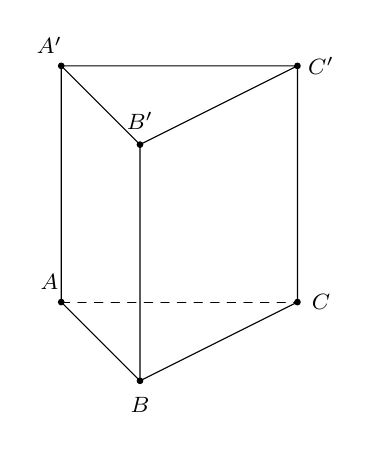
\begin{tikzpicture}[scale=1, font=\footnotesize, line join=round, line cap=round, >=stealth]
			\path (0,0) coordinate (A)	(1,-1) coordinate (B) (3,0) coordinate (C);
			\foreach \x in {A,B,C} \path (\x)+(0,3) coordinate (\x');
			\draw (A')--(A)--(B)--(C)--(C')--cycle (B)--(B') (A')--(B')--(C');
			\draw[dashed] (A)--(C);
			\foreach \x/\y in {A/120,B/-90,C/0,A'/120,B'/90,C'/0} \draw[fill=black] (\x) circle (1pt) node[shift=(\y:0.3)] {$\x$};
		\end{tikzpicture}
		
	}
	\loigiai{
		Dựa vào hình vẽ, đường thẳng $BB'$ song song với mặt phẳng $(ACC'A')$.
	}
\end{ex}

\begin{ex}%[1H4N3-2]%[Dự án C đề thi thử TN Môn Toán NH25-26 - Dot 4 - Hồng Trường Sơn]%[THPT Mai Anh Tuấn - Thanh Hóa]%[GVPB - Lê Hữu Kiệt]
	Cho hình lập phương $ABCD.A'B'C'D'$. Mệnh đề nào sau đây \textbf{sai}?
	\choice
	{$BD$ song song với $(A'C'D')$}
	{$BD$ song song với $(CB'D')$}
	{\True $BD$ vuông góc với $(ADD'A')$}
	{$BD$ vuông góc với $(ACC'A')$}
	\loigiai{
		\immini[thm]{
			$BD \parallel B'D'$ nên $BD$ song song với $(A'C'D')$, $BD$ song song với $(CB'D')$.\\
			$\heva{& BD\perp AC \\ & BD\perp AA'}$ nên $BD$ vuông góc với $(ACC'A')$.\\
			Mệnh đề sai là $BD$ vuông góc với $(ADD'A')$.
		}{
			\begin{tikzpicture}[>=stealth, line cap = round, font = \footnotesize, scale = 0.8]
				\path
				(0,0) coordinate (A)
				(-1.5,-1) coordinate (B)
				(2.5,-1) coordinate (C)
				($(A)+(C)-(B)$) coordinate (D)
				($(A)+(0,3.5)$) coordinate (A')
				($(A')+(B)-(A)$) coordinate (B')
				($(A')+(C)-(A)$) coordinate (C')
				($(A')+(D)-(A)$) coordinate (D')
				;
				\draw (B')--(C')--(D')--(A')--(B')--(B)--(C)--(C') (C)--(D)--(D');
				\draw[dashed] (A')--(A)--(B) (D)--(A);
				\foreach \x/\g in {A'/90,B'/140,C'/90,D'/90,A/140,B/-90,C/-90,D/-50} \fill (\x) circle (1.5pt) +(\g:3mm) node {$\x$};
			\end{tikzpicture}
		}
	}
\end{ex}

\begin{ex}%[1H4N3-2]%[TT-THPT Nguyễn Trung Thiên-Hà Tĩnh-L2-NH25-26]%[Bùi Quang Phú]%[GVPB2 PhanAnh]
\immini[thm]{Cho hình hộp $ABCD.A'B'C'D'$. Đường thẳng $AB$ song song với mặt phẳng nào sau đây?
	\choice
	{$\left(CC'A'A\right)$}
	{$\left(BB'C'C\right)$}
	{\True $\left(A'B'C'D'\right)$}
	{$\left(AA'D'D\right)$}}{\begin{tikzpicture}[scale=0.8,font={\footnotesize},>=stealth]	
		\path
		(0,0) coordinate (A)
		(4,0) coordinate (B)
		(1.8,1.6) coordinate (D)
		($(B)+(D)-(A)$) coordinate (C)
		($(A)+(0,2.5)$) coordinate (A')
		($(B)+(0,2.5)$) coordinate (B')
		($(C)+(0,2.5)$) coordinate (C')
		($(D)+(0,2.5)$) coordinate (D')
		;
		
		\draw[dashed] (A)--(D)--(C) (D)--(D');
		\draw (A)--(B)--(C)  (A)--(A') (B)--(B') (C)--(C') (A')--(B')--(C')--(D')--(A') ;
		% vẽ điểm
		\foreach \x/\g in {A/-90,B/-90,C/0,D/160,A'/180,B'/-30,C'/90,D'/90}
		\draw[fill=black] (\x) circle (1pt)+(\g:.3)
		node{$\x$};	
		
		\end{tikzpicture}}
	\loigiai{
	Vì $AB \parallel A'B'$ và $AB \not\subset \left(A'B'C'D'\right)$ nên $AB \parallel \left(A'B'C'D'\right)$.
	}
\end{ex}

\begin{ex}%[1H8H1-3]%[Dự án C đề thi thử TN Môn Toán NH25-26 - Đợt 4 - Đỗ Minh Phúc]%[Lần 1 Liên trường Hà Nội]%[GVPB - Lê Phúc]
	\immini[thm]{Cho hình lập phương $ABCD.A'B'C'D'$ (xem hình bên dưới). Góc giữa hai đường thẳng $A'C'$ và $D'C$ bằng
	\choice
	{$90^{\circ}$}
	{\True $60^{\circ}$}
	{$30^{\circ}$}
	{$45^{\circ}$}}
	{\begin{tikzpicture}[scale=0.7, font=\footnotesize, line join=round, line cap=round, >=stealth]
			\coordinate (A) at (0,0); 
			\coordinate (B) at (1,2);
			\coordinate (D) at (4,0);
			\coordinate (C) at ($(B)-(A)+(D)$);
			\coordinate (A') at ($(A)+(90:4)$);
			\coordinate (B') at ($(B)+(90:4)$);
			\coordinate (C') at ($(C)+(90:4)$);
			\coordinate (D') at ($(D)+(90:4)$);
			\draw (A)--(A')--(D')--(D)--(A) (A')--(B')--(C')--(D') (D)--(C)--(C')--(A') (A)--(D')--(C);
			\draw [dashed] (A)--(B)--(C) (B')--(B) (A)--(C);
			\foreach \x/\g in {A/-90,B/160,C/0,D/-90,A'/180,B'/90,C'/90,D'/120} \fill (\x) circle (1pt) +(\g:3mm) node{$\x$};
	\end{tikzpicture}}
	\loigiai{
		\immini[thm]{Trong hình lập phương $ABCD.A'B'C'D'$, ta có $A'C'\parallel A C$ (do $ACC'A'$ là hình chữ nhật).\\
			Do đó, góc giữa $\left(A'C',D'C\right)$ chính là góc giữa $\left(AC, D'C\right)$.\\
			Xét tam giác $ACD'$. Ta có
			$AC$, $CD'$, $AD'$ lần lượt là đường chéo của các hình vuông $ABCD$, $CDD'C'$, $ADD'A'$ nên $AC=CD'=AD'$.\\
			Khi đó, tam giác $ACD'$ có ba cạnh bằng nhau nên là tam giác đều.\\
			Suy ra $\widehat{ACD'}=60^{\circ}$.\\
			Vậy góc giữa hai đường thẳng $A'C'$ và $D'C$ bằng $60^{\circ}$.}{\begin{tikzpicture}[scale=0.8, font=\footnotesize, line join=round, line cap=round, >=stealth]
				\coordinate (A) at (0,0); 
				\coordinate (B) at (1,2);
				\coordinate (D) at (4,0);
				\coordinate (C) at ($(B)-(A)+(D)$);
				\coordinate (A') at ($(A)+(90:4)$);
				\coordinate (B') at ($(B)+(90:4)$);
				\coordinate (C') at ($(C)+(90:4)$);
				\coordinate (D') at ($(D)+(90:4)$);
				\draw (A)--(A')--(D')--(D)--(A) (A')--(B')--(C')--(D') (D)--(C)--(C')--(A') (A)--(D')--(C);
				\draw [dashed] (A)--(B)--(C) (B')--(B) (A)--(C);
				\foreach \x/\g in {A/-90,B/160,C/0,D/-90,A'/180,B'/90,C'/90,D'/120} \fill (\x) circle (1pt) +(\g:3mm) node{$\x$};
		\end{tikzpicture}}
	}
\end{ex}

\begin{ex}%[1H8H2-2][GV Biên Soạn: Thầy Hải Toán]%[GVPB - ThanhTa]
	Cho hình chớp $S.ABCD$ có đáy $ABCD$ là hình thoi tâm $O$, $SA=SC$, $SB=SD$. Trong các khẳng định sau khẳng định nào đúng?
	\choice
	{$SC\perp(ABCD)$}
	{\True $SO\perp(ABCD)$}
	{$SB\perp(ABCD)$}
	{$SA\perp(ABCD)$}
	\loigiai{
		\immini
		{
			Ta có $\heva{& SO\perp AC \\ & SO\perp BD \\ & AC\cap BD=\{O\}}\Rightarrow SO\perp (ABCD)$.	
		}
		{
			\begin{tikzpicture}[line join = round, line cap = round,>=stealth,font=\footnotesize,scale=1,declare function={ab=3;ad=5; gocA=-130;so=5;}]
				\path 
				(0,0) coordinate (A)
				(gocA:ab) coordinate (B)
				(ad,0) coordinate (D)
				($(D)-(A)+(B)$) coordinate (C)
				(intersection of A--C and B--D) coordinate (O)
				($(O)+(0,so)$) coordinate (S)
				;
				\draw (S)--(B)--(C)--(D)--(S)--(C);
				\draw[dashed] (B)--(A)--(D) (S)--(A)--(C) (B)--(D) (S)--(O);
				\foreach \x/\gm in {A/-90,B/-90,C/-90,D/0,S/90,O/-90} \fill (\x) circle (1pt) ($(\x)+(\gm:3.5mm)$)node{$\x$};
			\end{tikzpicture}		
		}
	}
\end{ex}

\begin{ex}%[1H8H2-2]%[Dự án C đề thi thử TN Môn Toán NH25-26 - Dot 4 - Bui Luong Phuc]%[THPT Lê Thánh Tông-TPHCM]%[GVPB - Viet Hoang Pham]
Cho hình chóp $S.ABCD$ có đáy là hình vuông, cạnh bên $SA$ vuông góc với đáy $(ABCD)$. Phát biểu nào sau đây là \textbf{sai}?
\choice
{\True $CD \perp (SBC)$}
{$SA \perp (ABC)$}
{$BC \perp (SAB)$}
{$BD \perp (SAC)$}
\loigiai{
\begin{center}
\begin{tikzpicture}[scale=0.8, font=\footnotesize, line join=round, line cap=round, >=stealth]
\coordinate (A) at (0,0);
\coordinate (B) at (-1.5,-1.5);
\coordinate (D) at (3,0);
\coordinate (C) at ($(B)+(D)-(A)$);
\coordinate (S) at (0,3);
\draw (S)--(B)--(C)--(D)--(S)--(C);
\draw[dashed] (S)--(A)--(B) (A)--(D) (A)--(C) (B)--(D);
\foreach \p/\pos in {S/above, A/left, B/below left, C/below, D/right}
\fill (\p) circle (1pt) node[\pos] {$\p$};
\end{tikzpicture}
\end{center}
%Ta có $\heva{&AB\parallel CD\\&AB\not\perp SB} \Rightarrow CD\not\perp SB \Rightarrow CD \not\perp (SBC)$.\\
Ta có $\heva{&CD\perp AD\\&CD\perp SA} \Rightarrow CD \perp (SAD)$\quad ($1$).\\
Mặt khác, $(SAD)\not \parallel (SBC)$ (hai mặt phẳng này cắt nhau)\quad ($2$).\\
Từ ($1$) và ($2$) suy ra $CD \not\perp (SBC)$.
}
\end{ex}

\begin{ex}%[TT Cụm 5 - Ninh Bình-NH25-26]%[Nguyễn Chiến]%[Phản biện 1: Nguyễn Tấn Tài]%[1H8H4-5]
	Cho hình chóp đều $S.ABCD$ có cạnh đáy $2a$, cạnh bên $4a$. Tính độ dài đường cao hình chóp.
	\choice
	{$3a$}
	{$2a$}
	{\True $a\sqrt{14}$}
	{$a\sqrt{15}$}
	\loigiai{
		Gọi $O$ là tâm của hình vuông $ABCD$.
		\begin{center}
			\begin{tikzpicture}[line join = round, line cap=round,>=stealth,font=\footnotesize,scale=1]
				\def\a{4}
				\def\b{2}
				\def\h{4}
				\def\g{30}
				\path
				(0,0) coordinate (B)
				(0:\a) coordinate (C)
				(\g:\b) coordinate (A)
				($(A)+(C)-(B)$) coordinate (D)
				($(A)!.5!(C)$) coordinate (O)
				(O)++(90:\h) coordinate (S)
				;
				\draw (S)--(B)--(C)--(D)--(S)--(C);
				\draw[dashed] (O)--(S)--(A)--(B)--(D)--(A)--(C);
				\path (O) pic[draw,angle radius=5pt,angle eccentricity=2]{right angle = S--O--B};
				\foreach \x/\g in {A/135,B/-135,C/-45,D/-45,S/90,O/45}\fill (\x) circle (1pt) + (\g:0.3) node {$\x$};
			\end{tikzpicture}
		\end{center}
		Do $S.ABCD$ là hình chóp đều nên $SO$ là đường cao của hình chóp.\\
		Cạnh đáy của hình chóp là $AB=2a$.\\
		Đường chéo của hình vuông $ABCD$ là $AC=AB\sqrt{2}=2a\sqrt{2}$.\\
		Tâm $O$ của hình vuông là trung điểm của $AC$.\\
		Suy ra $AO=\dfrac{1}{2}AC=a\sqrt{2}$.\\
		Cạnh bên của hình chóp là $SA=4a$.\\
		Xét tam giác $SOA$ vuông tại $O$, ta có 
		$$SA^2=SO^2+AO^2\Rightarrow (4a)^2=SO^2+(a\sqrt{2})^2\Rightarrow SO^2=14a^2.$$
		Suy ra $SO=a\sqrt{14}$.\\
		Vậy độ dài đường cao hình chóp là $a\sqrt{14}$.
	}
\end{ex}

\begin{ex}%[1H8H6-1]%[Dự án đề TT Toán NH25-26-Dot 3- Bùi Lương Phúc]%[Cụm 13-Hải Phòng]%[GVPB - Viet Hoang Pham]
\immini[thm]{
Cho hình chóp $S.ABCD$ có đáy $ABCD$ là hình vuông cạnh $a$, $SA\perp (ABCD)$ và $SA=a\sqrt{3}$. Số đo góc giữa $SB$ và $(ABCD)$ bằng
\choice
{\True $60^\circ$}
{$30^\circ$}
{$90^\circ$}
{$45^\circ$}
}{
\begin{tikzpicture}[line join=round,line cap=round,scale=1,font=\footnotesize,>=stealth]
\coordinate (D) at (0,0);
\coordinate (C) at (3,0);
\coordinate (A) at (1,1.5);
\coordinate (B) at ($(A)+(C)-(D)$);
\coordinate (S) at ($(A)+(0,2.5)$);
\draw [dashed](S)--(A)--(B) (A)--(D);
\draw (B)--(S)--(D)--(C)--cycle (S)--(C) ;
\foreach \p/\g in {A/150,B/45,C/-45,D/-135,S/90}
\node at ($(\p)+(\g:0.3)$){$\p$};
\draw pic[draw,angle radius=2.5mm] {right angle = S--A--B}; 
\end{tikzpicture}
}
\loigiai{
Vì $SA\perp(ABCD)$ nên $AB$ là hình chiếu của $SB$ lên $(ABCD)$.\\
Do đó
\[
\left(SB,(ABCD)\right)=(SB,AB)=\widehat{SBA}.
\]
Xét tam giác $SAB$ vuông tại $A$ với $SA=a\sqrt{3}$, $AB=a$ ta có
\[
\tan\widehat{SBA}=\dfrac{SA}{AB}=\dfrac{a\sqrt{3}}{a}=\sqrt{3}
\Rightarrow \widehat{SBA}=60^\circ.
\]
Vậy $\left(SB,(ABCD)\right)=60^\circ$.
}
\end{ex}

\begin{ex}%[1H8H6-1]%[Dự án đề thi thử NH25-26]%[THPT Chuyên Phan Bội Châu - Nghệ An]%[GVPB2 Khắc Thiên]
	\immini[thm]{Cho hình lập phương $ABCD.A'B'C'D'$. Tính góc giữa hai đường thẳng $AB$ và $A'C'$.
		\choice
		{\True $45^\circ$}
		{$90^\circ$}
		{$60^\circ$}
		{$30^\circ$}}{	
		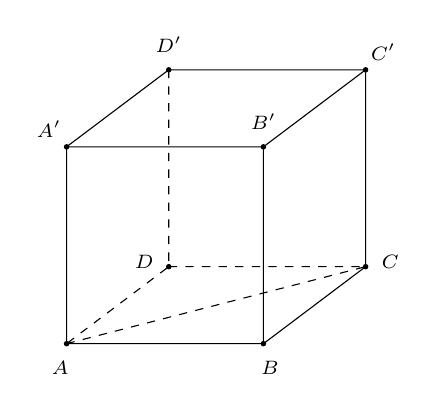
\begin{tikzpicture}[declare function={r=2.5;},font=\scriptsize]
			\path (0:0) coordinate (A)
			(0:r) coordinate (B)
			++(37:{0.65*r}) coordinate (C)
			++(180:r) coordinate (D)
			\foreach \x in {A,B,C,D}{(\x)++(90:r) coordinate (\x_1)};
			\draw[dashed] (D_1)--(D)--(A) (A)--(C)
			(D)--(C);
			\draw (A)--(B)--(C)
			(A)--(A_1)
			(B)--(B_1)
			(C)--(C_1)
			(A_1)--(B_1)--(C_1)--(D_1)--cycle;
			\foreach \x/\goc/\t in {A/255/A,B/-75/B,C/10/C,D/170/D,A_1/135/A',B_1/90/B',
				C_1/45/C',D_1/90/D'}{
				\fill (\x) circle (1pt) node[shift={(\goc:9pt)}]{$\t$};
			}
	\end{tikzpicture}}
	\loigiai{
		Ta có $A'C' \parallel AC$ nên $\left(AB, A'C'\right) = \left(AB, AC\right) = \widehat{BAC} = 45^\circ$ (do tứ giác $ABCD$ là hình vuông).
	}
\end{ex}

\begin{ex}%[1H8H6-1][Dự án C đợt 3 NH25-26- Nguyễn Hữu Đức]%[SỞ GIÁO DỤC - TUYÊN QUANG]%[GVPB: Thanh Phát]
	Cho hình chóp $S.ABC$ có $SA$ vuông góc với mặt phẳng $(ABC)$, $SA = a\sqrt{2}$, $AB = a\sqrt{2}$ (xem hình dưới).
	\begin{center}
		\begin{tikzpicture}[scale=0.65,font=\footnotesize,line join=round
			,line cap=round,>=stealth]
			\path
			(0,0) coordinate (A)
			++(-60:3) coordinate (B)
			(5,0) coordinate (C)
			($(A)+(0,4)$) coordinate (S);
			\foreach \i in {C,B,A}{\draw (S)--(\i);}
			\draw (C)--(B)--(A);
			\draw[dashed](C)--(A);% (I)--(J);
			\foreach \i/\g in {S/90,A/180,B/-90,C/0}
			\fill[black] (\i) circle(1pt)+(\g:4mm)node[scale=1]{$\i$};
		\end{tikzpicture}
	\end{center}
	Góc giữa đường thẳng $SB$ và mặt phẳng $(ABC)$ bằng  
	\choice
	{\True $45^\circ$}  
	{$30^\circ$}  
	{$90^\circ$}  
	{$60^\circ$}  
	\loigiai{
		Vì $SA \perp (ABC)$ nên hình chiếu của $SB$ lên mặt phẳng $(ABC)$ là $AB$. \\ 
		Do đó, góc giữa $SB$ và $(ABC)$ là góc $\widehat{SBA}$.\\  
		Xét tam giác $SAB$ vuông tại $A$, ta có\\  
		$\tan \widehat{SBA} = \dfrac{SA}{AB} = \dfrac{a\sqrt{2}}{a\sqrt{2}} = 1$.\\  
		Suy ra $\widehat{SBA} = 45^\circ$.  
	}
\end{ex}

\begin{ex}%[1H8H7-2]%[Dự án C đề thi thử TN Môn Toán NH25-26 - Đợt 4 - Đỗ Minh Phúc]%[Lần 1 Liên trường Hà Nội]%[GVPB - Lê Phúc]
	Cho hình chóp $S.ABC$ có đáy $ABC$ là tam giác đều cạnh bằng $6$. Cạnh bên $SA=5$ và $SA$ vuông góc với mặt phẳng $(ABC)$. Thể tích của khối chóp $S.ABC$ bằng.
	\choice
	{$45\sqrt{3}$}
	{$9\sqrt{3}$}
	{$36\sqrt{3}$}
	{\True $15\sqrt{3}$}
	\loigiai{
		\immini[thm]{Ta có $S_{\triangle A B C}=\dfrac{6^2 \sqrt{3}}{4}=\dfrac{36 \sqrt{3}}{4}=9 \sqrt{3}$.\\
			Lại có chiều cao của khối chóp là $h=SA=5$ nên thể tích của khối chóp đã cho là $V=\dfrac{1}{3} \cdot 9 \sqrt{3} \cdot 5=15\sqrt{3}$.}{\begin{tikzpicture}[scale=0.7, font=\footnotesize, line join=round, line cap=round, >=stealth]
				\coordinate (A) at (0,0); 
				\coordinate (B) at (3,-2);
				\coordinate (C) at (5,0);
				\coordinate (S) at ($(A)+(90:4)$);
				\draw (S)--(A)--(B)--(C)--(S)--(B);
				\draw [dashed] (A)--(C);
				\foreach \x/\g in {A/180,B/-90,C/0,S/90} \fill (\x) circle (1pt) +(\g:3mm) node{$\x$};
		\end{tikzpicture}}
	}
\end{ex}

\begin{ex}%[Dự án C - Đợt 3 - Sở Giáo Dục Sơn La]%[GV biên soạn: Nhật Thiện - GV phản biện: Nguyễn Tiến]%[1H8H7-2]
	Cho hình chóp $S.ABC$ có $SA\perp (ABC)$; $SA=3$; $\triangle ABC$ vuông cân tại $A$ với $AB=4$. Thể tích khối chóp $S.ABC$ bằng
	\choice
	{$48$}
	{$16$}
	{\True $8$}
	{$24$}
	\loigiai{
		Thể tích khối chóp 
		$$V=\dfrac{1}{3}\cdot S_{ABC}\cdot SA=\dfrac{1}{3}\cdot \dfrac{1}{2}\cdot AB^2\cdot SA=\dfrac{1}{3}\cdot \dfrac{1}{2}\cdot 4^2\cdot 3=8.$$
	}
\end{ex}

\begin{ex}%[1H8H7-3]%[Dự án đề TT Toán NH25-26-Dot 3-PhucChuong]%[THPT Lê Quý Đôn - Đống Đa - Hà Nội]%[GVPB - Phan Quốc Trí]
 	Cho khối chóp $S.ABCD$ có đáy $ABCD$ là hình chữ nhật với $BC=3a$, $CD=4a$. Cạnh bên $SC$ vuông góc với mặt phẳng đáy và $SC=5a$. Thể tích $V$ của khối chóp $S.ABCD$ là
 	\choice
 	{$V=30a^3$}
 	{$V=10a^3$}
 	{$V=60a^3$}
 	{\True $V=20a^3$}
 	\loigiai{
 		Thể tích của khối chóp là $V=\dfrac{1}{3}S_{ABCD} \cdot SC = \dfrac{1}{3} \cdot 3a \cdot 4a \cdot 5a = 20a^3$.
 	}
 \end{ex}

\begin{ex}%[1H8H7-3]%[Dự án đề TT Toán NH25-26-Dot 3-PhucChuong]%[THPT Trần Nhân Tông - Hà Nội]%[GVPB - Phan Quốc Trí]
	Cho hình chóp tứ giác $S.ABCD$ có đáy $ABCD$ là hình vuông cạnh bằng $1$ dm, cạnh bên $SA$ vuông góc với mặt phẳng đáy và $SA=\sqrt{2}$ dm. Thể tích $V$ của khối chóp $S.ABCD$ là
	\choice
	{\True $V=\dfrac{\sqrt{2}}{3}$ dm$^3$}
	{$V=\dfrac{\sqrt{2}}{4}$ dm$^3$}
	{$V=\dfrac{\sqrt{2}}{6}$ dm$^3$}
	{$V=\sqrt{2}$ dm$^3$}
	\loigiai{
		\immini[thm]{Thể tích 
			\begin{eqnarray*}
				V_{S.ABCD} &=& \dfrac{1}{3}\cdot SA\cdot S_{ABCD} = \dfrac{1}{3}\cdot SA\cdot AB^2 \\
				&=& \dfrac{1}{3}\cdot \sqrt{2}\cdot 1^2 = \dfrac{\sqrt{2}}{3} \text{ dm}^3.
			\end{eqnarray*}
		}{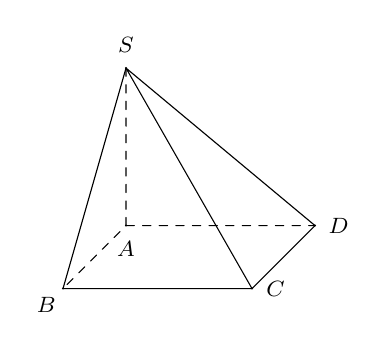
\begin{tikzpicture}[scale=.4, font=\footnotesize, line join=round, line cap=round, >=stealth]
				\path (0,0) coordinate (A)++(-2,-2) coordinate (B)++(6,0) coordinate (C)++(2,2) coordinate (D) %PC
				(A)++(0,5) coordinate (S);
				\draw[dashed] (S)--(A)--(B) (A)--(D);
				\draw (S)--(B)--(C)--(D)--(S)--(C);
				\foreach \x/\y in {S/90,A/-90,B/-135,C/0,D/0}
				{\fill (\x)node[shift={(\y:3mm)}]{$\x$} circle (1pt);}
		\end{tikzpicture}}
	}
\end{ex}

\begin{ex}%[Đề thi thử môn Toán THPT Cổ Loa, năm học 2025-2026]%[Đỗ Minh Phúc]%[1H8H7-4]%[PB1: Lê Phúc]
	Cho hình lăng trụ đứng $ABC.A'B'C'$ có đáy $ABC$ là tam giác vuông tại $B$ và $AA'=4$, $AB=5$, $BC=6$. Thể tích của khối lăng trụ $ABC.A'B'C'$ bằng
	\choice
	{$30$}
	{\True $60$}
	{$20$}
	{$120$}
	\loigiai{
		\immini[thm]{Ta có \[V_{ABC.A'B'C'}=S_{\triangle ABC} \cdot AA'=\dfrac{1}{2} AB \cdot BC \cdot AA'=\dfrac{1}{2} \cdot 5 \cdot 6 \cdot 4=60.\]}{\begin{tikzpicture}[scale=0.8, font=\footnotesize, line join=round, line cap=round, >=stealth]
				\coordinate (A) at (0,0); 
				\coordinate (B) at (3,-2);
				\coordinate (C) at (4,0);
				\coordinate (A') at ($(A)+(90:4)$);
				\coordinate (B') at ($(B)+(90:4)$);
				\coordinate (C') at ($(C)+(90:4)$);
				\draw (A')--(B')--(C')--(A') (A)--(A')node[left,midway]{$4$} (B)--(B') (C)--(C') (A)--(B)node[below,midway]{$5$}--(C)node[right,midway]{$6$};
				\draw [dashed] (A)--(C);
				\foreach \x/\g in {A/180,B/-90,C/0,A'/180,B'/0,C'/0} \fill (\x) circle (1pt) +(\g:3mm) node{$\x$};
				\draw pic[draw, angle radius = 5pt]{right angle = A--B--C};
		\end{tikzpicture}}
	}
\end{ex}

\begin{ex}%[1H8N7-1]%[Dự án đề thi thử NH25-26]%[THPT Chuyên Phan Bội Châu - Nghệ An]%[GVPB2 Khắc Thiên]
	Cho hình chóp có diện tích đáy bằng $10$ và chiều cao bằng $6$. Tính thể tích khối chóp đã cho.
	\choice
	{$30$}
	{$16$}
	{\True $20$}
	{$60$}
	\loigiai{
		Thể tích khối chóp là $V = \dfrac{1}{3}Bh = \dfrac{1}{3} \cdot 10 \cdot 6 = 20$.
	}
\end{ex}

\begin{ex}%[1H8N7-2]%[Dự án C đề thi thử TN Môn Toán NH25-26 - Dot 4 - Thy Nguyen Vo Diem]%[Liên trường THPT cụm 09 - Đợt 2 - Hà Nội]%[GVPB - Thanh Phát]
	Khối chóp $S.ABC$ có chiều cao bằng $3$, diện tích đáy bằng $10$. Thể tích khối chóp $S.ABC$ bằng
	\choice
	{$2$}
	{\True $10$}
	{$15$}
	{$30$}
	\loigiai{
		Thể tích của khối chóp $S.ABC$ là 
		$$V = \dfrac{1}{3}Bh=\dfrac{1}{3} \cdot 10 \cdot 3 = 10.$$
	}
\end{ex}

\begin{ex}%[1H8N7-3]%[TT-THPT Nguyễn Trung Thiên-Hà Tĩnh-L2-NH25-26]%[Bùi Quang Phú]%[GVPB2 PhanAnh]
Cho hình chóp $S.ABCD$ có đáy $ABCD$ là hình vuông cạnh $a$. Biết $SA \perp (ABCD)$ và $SA=a\sqrt{3}$. Thể tích khối chóp $S.ABCD$ là
	\choice
	{$a^3\sqrt{3}$}
	{\True $\dfrac{a^3\sqrt{3}}{3}$}
	{$\dfrac{a^3}{4}$}
	{$\dfrac{a^3\sqrt{3}}{12}$}
	\loigiai{
	Diện tích hình vuông $ABCD$ là $a^2$.\\
	Thể tích khối chóp $S.ABCD$ là $V=\dfrac{1}{3}\cdot S_{ABCD} \cdot SA=\dfrac{1}{3} \cdot a^2 \cdot a\sqrt{3}=\dfrac{a^3\sqrt{3}}{3}$.
	}
\end{ex}

\begin{ex}%[1H8N7-4]%[Dự án C đề thi thử TN Môn Toán NH25-26 - Dot 4 - Hồng Trường Sơn]%[THPT Mai Anh Tuấn - Thanh Hóa]%[GVPB - Lê Hữu Kiệt]
	Lăng trụ tam giác đều có độ dài tất cả các cạnh bằng $2$. Thể tích khối lăng trụ đã cho bằng
	\choice
	{\True $2\sqrt{3}$}
	{$8\sqrt{3}$}
	{$4\sqrt{3}$}
	{$\sqrt{3}$}
	\loigiai{
		\immini[thm]{
			Diện tích đáy tam giác đều là
			$$S=\dfrac{2^2\sqrt{3}}{4}=\sqrt{3}.$$
			Thể tích khối lăng trụ đã cho bằng
			$$V=S\cdot h=\sqrt{3}\cdot 2=2\sqrt{3}.$$
		}{
			\begin{tikzpicture}[line join = round,>=stealth, line cap = round, font = \footnotesize, scale = 0.8]
				\path
				(0,0) coordinate (A)
				(1.5,-1) coordinate (B)
				(4,0) coordinate (C)
				($(A)+(0,3.5)$) coordinate (A')
				($(A')+(B)-(A)$) coordinate (B')
				($(A')+(C)-(A)$) coordinate (C')
				;
				\draw (B')--(C')--(A')--(B')--(B)--(A)--(A') (B)--(C)--(C');
				\draw[dashed] (C)--(A);
				\foreach \x/\g in {A'/90,B'/90,C'/90,A/-140,B/-90,C/-50} \fill (\x) circle (1.5pt) +(\g:3mm) node {$\x$};
			\end{tikzpicture}
		}
	}
\end{ex}

\begin{ex}%[2D1H1-1]%[Dự án đề TT Toán NH25-26-Dot 3- Bùi Lương Phúc]%[Cụm 13-Hải Phòng]%[GVPB - Viet Hoang Pham]
Cho hàm số $y=f(x)$ có đạo hàm $f'(x)=(x-2)(x+1)$, $\forall x\in\mathbb{R}$. Mệnh đề nào dưới đây đúng?
\choice
{Hàm số đã cho đồng biến trên $(-1;+\infty)$}
{Hàm số đã cho đồng biến trên $(-\infty;2)$}
{Hàm số đã cho đồng biến trên $(-1;2)$}
{\True Hàm số đã cho nghịch biến trên $(-1;2)$}
\loigiai{
Ta có $f'(x)=0\Leftrightarrow (x-2)(x+1)=0\Leftrightarrow\hoac{&x=2\\&x=-1.}$\\
Bảng xét dấu $f'(x)$
\begin{center}

\begin{tikzpicture}
\tkzTabInit[nocadre=true,lgt=1.3,espcl=2.5]
{$x$/1,$f'(x)$/1}
{$-\infty$,-1,2,$+\infty$}
\tkzTabLine{,+,0,-,0,+}
\end{tikzpicture}
\end{center}
Suy ra hàm số nghịch biến trên khoảng $(-1;2)$.
}
\end{ex}

\begin{ex}%[2D1H1-1]%[Đề thi thử môn Toán TRƯỜNG THPT Hàm Rồng năm học 2025-2026]%[Dương Phạm - GVPB2 Đỗ Minh Vũ]
	Hàm số $y=\dfrac{x^2-x+2}{x+1}$ nghịch biến trên khoảng nào sau đây?
	\choice
	{$(-\infty; -3)$}
	{$(-3; 1)$}
	{$(-1; +\infty)$}
	{\True $(-1; 1)$}
	\loigiai{
		Ta có $y = \dfrac{x^2 - x + 2}{x + 1}$, điều kiện $x \neq -1$. \\
		$\Rightarrow y' = \dfrac{x^2 + 2x - 3}{(x + 1)^2}$, điều kiện $x \neq -1$. \\
		Để hàm số $y = \dfrac{x^2 - x + 2}{x + 1}$ nghịch biến thì $y' \leq 0$ 
	\allowdisplaybreaks	\begin{eqnarray*}
		&\Leftrightarrow& \dfrac{x^2 + 2x - 3}{(x + 1)^2} \leq 0 \\
		&\Rightarrow& x^2 + 2x - 3 \leq 0 \\
		&\Leftrightarrow& -3 \leq x \leq 1. 
		\end{eqnarray*}
		Kết hợp với điều kiện xác định, suy ra hàm số $y = \dfrac{x^2 - x + 2}{x + 1}$ nghịch biến trên khoảng $(-3; -1)$ và $(-1; 1)$. 
	}
\end{ex}

\begin{ex}%[2D1H1-1]%[Dự án C đề thi thử TN Môn Toán NH25-26 - Dot 4 - Huỳnh Hồ Hải]%[PhanBoiChau-KhanhHoa]%[GVPB - Phạm Văn Long]	
	Hàm số nào sau đây đồng biến trên $\mathbb{R}$?
	\choice
	{$y=-x^3+3x+5$}
	{$y=-x^3+2x-5$}
	{\True $y=x^3+x+5$}
	{$ y=\dfrac{2x-1}{x+1}$}
	\loigiai{
		\begin{itemize}
			\item Xét hàm số $y=\dfrac{2x-1}{x+1}$ có tập xác định: $\mathscr{D}=\mathbb{R}\setminus\left\{-1\right\}$ nên không đồng biến trên $\mathbb{R}$.
			\item Xét hàm số $y=-x^3+2x-5$ có tập xác định: $\mathscr{D}=\mathbb{R}$ và $y'=-3x^2+2$.\\
			Xét $y'=0 \Leftrightarrow x=\pm \dfrac{\sqrt{6}}{3}$ nên $y'$ đổi dấu khi qua các nghiệm. Hàm số không đồng biến trên $\mathbb{R}$.
			\item Xét hàm số $y=-x^3+3x+5$ có tập xác định: $\mathscr{D}=\mathbb{R}$ và $y'=-3x^2+3$.\\
			Xét $y'=0\Leftrightarrow x=\pm 1$ nên $y'$ đổi dấu khi qua các nghiệm. Hàm số không đồng biến trên $\mathbb{R}$.
			\item 	Xét hàm số $y=x^3+x+5$ có tập xác định: $\mathscr{D}=\mathbb{R}$.
			Ta có $ y'=3x^2+1>0$, với $\forall x\in\mathbb{R}$. Vậy hàm số luôn đồng biến trên $\mathbb{R}$.			
	\end{itemize}}
\end{ex}

\begin{ex}%[2D1H1-5]%[Dự án C đề thi thử TN Môn Toán NH25-26 - Dot 4 - Hồng Trường Sơn]%[THPT Mai Anh Tuấn - Thanh Hóa]%[GVPB - Lê Hữu Kiệt]
	Giả sử sự lây lan của một loại virus ở một địa phương có thể được mô hình hóa bằng hàm số $N(t)=-t^3+12t^2$, $0\le t\le 12$ trong đó $N$ là số người bị nhiễm bệnh (tính bằng trăm người) và $t$ là thời gian (tuần). Hỏi số người bị nhiễm bệnh tăng trong khoảng thời gian nào?
	\choice
	{\True $(0;8)$}
	{$(0;10)$}
	{$(8;12)$}
	{$(8;10)$}
	\loigiai{
		Xét hàm số $N(t)=-t^3+12t^2$, $0\le t\le 12$.\\
		Ta có $N'(t)=-3t^2+24t$; $N'(t)=0 \Leftrightarrow \hoac{& t=0 \\ & t=8.}$\\
		Bảng biến thiên
		\begin{center}
			
\begin{tikzpicture}
				\tkzTabInit[nocadre=false,lgt=1.5,espcl=2.5,deltacl=.5]
				{$t$ /.7, $N’(t)$ /.7,$N(t)$ /2}
				{$0$ , $8$, $12$}
				\tkzTabLine{,+,0,-,}
				\tkzTabVar{-/$ $ ,+/ $ $ ,-/$ $}
			\end{tikzpicture}
		\end{center}
		Từ bảng biến thiên ta thấy số người bị nhiễm bệnh tăng trong khoảng thời gian $t\in (0;8)$.
	}
\end{ex}

\begin{ex}%[2D1H2-1]%[Dự án C đề thi thử TN Môn Toán NH25-26 - Dot 4 - Thy Nguyen Vo Diem]%[Liên trường THPT cụm 09 - Đợt 2 - Hà Nội]%[GVPB - Thanh Phát]
	Cho hàm số $f(x)$ xác định trên $\mathbb{R}$, có $f'(x) = x(x-1)(x+2)^2$. Số điểm cực trị của hàm số $f(x)$ là
	\choice
	{$3$}
	{$1$}
	{\True $2$}
	{$4$}
	\loigiai{
		Ta có $f'(x) = 0 \Leftrightarrow x(x-1)(x+2)^2 = 0 \Leftrightarrow \hoac{&x=0 &&\text{(bội lẻ)}\\
			&x=1 &&\text{(bội lẻ)} \\
			&x=-2 &&\text{(bội chẵn).}}$\\
		Phương trình $f'(x)=0$ có $2$ nghiệm bội lẻ nên hàm số $f(x)$ có $2$ điểm cực trị.
	}
\end{ex}

\begin{ex}%[2D1H2-2]%[Dự án đề TT Toán NH25-26-Dot 3-PhucChuong]%[THPT Lê Quý Đôn - Đống Đa - Hà Nội]%[GVPB - Phan Quốc Trí]
 	Cho hàm số $y = f(x)$ liên tục trên $\mathbb{R}$ và có bảng biến thiên như hình dưới.
 	\begin{center}
 		
\begin{tikzpicture}[thick]
 			\tkzTabInit[lgt=1.5,espcl=3.5,nocadre=False,lw=1pt]{$x$/1, $f'(x)$/1, $f(x)$/2}
 			{$-\infty$,$0$,$1$,$+\infty$}
 			\tkzTabLine{,+,0,-,0,+,}
 			\tkzTabVar{-/$-\infty$, +/$-2$, -/$-3$, +/$+\infty$}	
 		\end{tikzpicture}
 	\end{center}
 	Hàm số đạt cực đại tại điểm
 	\choice
 	{$x = 1$}
 	{$x = -3$}
 	{$x = -2$}
 	{\True $x = 0$}
 	\loigiai{
 		Dựa vào bảng biến thiên, ta thấy hàm số đạt cực đại tại $x = 0$.
 	}
 \end{ex}

\begin{ex}%[2D1H2-2]%[Dự án C đề thi thử TN Môn Toán NH25-26 - Dot 4 - Huỳnh Hồ Hải]%[PhanBoiChau-KhanhHoa]%[GVPB - Phạm Văn Long]	
	Cho hàm số $y=f(x)$ liên tục trên $\mathbb{R}$ và có đồ thị như hình vẽ.
	\begin{center}
		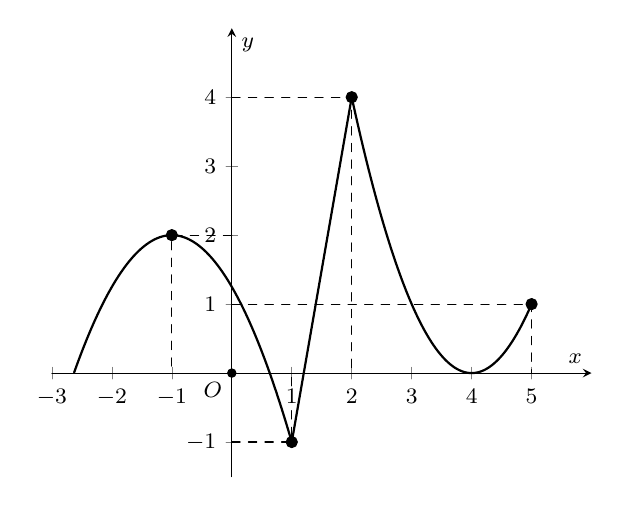
\begin{tikzpicture}[thick,line join = round, line cap = round,>=stealth,font=\footnotesize]
		%Thêm gói lệnh \usepackage{pgfplots}
		%Thêm gói lệnh\pgfplotsset{compat=1.18}
			\begin{axis}[
				axis lines = middle, % trục tọa độ đi qua gốc
				xlabel = {$x$},
				ylabel = {$y$},
				minor tick num=0, % lưới
				xmin = -3, xmax = 6,
				ymin = -1.5, ymax = 5,
				xtick = {-3,-2,-1,0,1,2,3,4,5},
				ytick = {-1,0,1,2,3,4},
				samples = 100
				]
				\addplot[domain=-2.63:1, thick] { -3/4*(x+1)^2 + 2 };
				\addplot[domain=1:2, thick] {5*x-6};
				\addplot[domain=2:5, thick] {(x-4)^2};
				% vẽ điểm đặc biệt
				\addplot[only marks] coordinates {(-1,2) (1,-1) (2,4) (5,1)};
				\addplot[only marks, mark size=1.5pt] coordinates {(0,0)}
				node[below left] {$O$};
				\addplot[dashed] coordinates {(0,2) (-1,2) (-1,0)};
				\addplot[dashed] coordinates {(0,-1) (1,-1) (1,0)};
				\addplot[dashed] coordinates {(0,4) (2,4) (2,0)};
				\addplot[dashed] coordinates {(0,1) (5,1) (5,0)};
			\end{axis}
		\end{tikzpicture}
	\end{center}
	Gọi $M$, $m$ lần lượt là giá trị lớn nhất và giá trị nhỏ nhất của hàm số đã cho trên đoạn $\left[0;5\right]$. Tính $P=M+m$.	
	\choice
	{$P=5$}
	{\True $P=3$}
	{$P=4$}
	{$P=2$}
	\loigiai{
		Nhìn vào đồ thị ta thấy $M=4$, $ m=-1$. Vậy $P=M+m=4+(-1)=3$.}
\end{ex}

\begin{ex}%[TT Cụm 5 - Ninh Bình-NH25-26]%[Nguyễn Chiến]%[Phản biện 1: Nguyễn Tấn Tài]%[2D1H3-1]
	Cho hàm số $y=f(x)$ có đạo hàm $f'(x)=(2x-1)(x+1)$. Hàm số $y=f(x)$ có giá trị lớn nhất trên $[-2;0]$ bằng
	\choice
	{$f\left(-\dfrac{1}{2}\right)$}
	{\True $f(-1)$}
	{$f(0)$}
	{$f(-2)$}
	\loigiai{
		Ta có $f'(x)=(2x-1)(x+1)=0\Rightarrow \hoac{&x=\dfrac{1}{2}\\&x=-1.}$\\
		Bảng biến thiên
		\begin{center}
			
\begin{tikzpicture}
				\tkzTabInit[nocadre=false,lgt=1.2,espcl=2.5,deltacl=0.6]
				{$x$ /0.6, $f'(x)$ /0.6, $f(x)$ /2}
				{$-\infty$,$-1$,$\frac{1}{2}$,$+\infty$}
				\tkzTabLine{ ,+,$0$,-,$0$,+, }
				\tkzTabVar{-/$-\infty$,+/$f(-1)$,-/$f\left(\dfrac{1}{2}\right)$,+/$+\infty$}
			\end{tikzpicture}
		\end{center}
		Từ bảng biến thiên ta thấy $\max\limits_{x\in [-2;0]}f(x)=f(-1)$.
	}
\end{ex}

\begin{ex}%[2D1H3-1]%[Dự án đề TT Toán NH25-26-Dot 3- Bùi Lương Phúc]%[Cụm 13-Hải Phòng]%[GVPB - Viet Hoang Pham]
Giá trị lớn nhất của hàm số $y=x^3-7x^2+11x-2$ trên đoạn $[0;3]$ là
\choice
{$-5$}
{$-2$}
{\True $3$}
{$5$}
\loigiai{
Ta có $y'=3x^2-14x+11$.\\
$y'=0 \Leftrightarrow \hoac{&x=1 \in [0;3]\\&x=\dfrac{11}{3}\notin[0;3]}$.\\
Tính $y(0)=-2$, $y(1)=3$, $y(3)=-5$.\\
Suy ra $\max\limits_{[0;3]}y=3$.
}
\end{ex}

\begin{ex}%[2D1H3-1]%[Dự án đề TT Toán NH25-26-Dot 3-PhucChuong]%[THPT Lê Quý Đôn - Đống Đa - Hà Nội]%[GVPB - Phan Quốc Trí]
 	Giá trị lớn nhất của hàm số $f(x)=\dfrac{2x-5}{x-1}$ trên đoạn $[2;5]$ là
 	\choice
 	{$-1$}
 	{$\dfrac{1}{2}$}
 	{\True $\dfrac{5}{4}$}
 	{$1$}
 	\loigiai{
 		Ta có $f'(x)=\dfrac{3}{(x-1)^2} > 0, \forall x \in [2;5]$ nên hàm số $f(x)$ đồng biến trên đoạn $[2;5]$.\\
 		Vậy $\max\limits_{[2;5]} f(x) = f(5) = \dfrac{2 \cdot 5 - 5}{5 - 1} = \dfrac{5}{4}$.
 	}
 \end{ex}

\begin{ex}%[2D1H4-1]%[Dự án C đợt 3 NH25-26- Nguyễn Hữu Đức]%[SỞ GIÁO DỤC - TUYÊN QUANG]%[GVPB: Thanh Phát]
	Tiệm cận xiên của đồ thị hàm số $y = x+1 - \dfrac{1}{x-2}$ là đường thẳng có phương trình  
	\choice
	{$y = x$}  
	{$x = 2$}  
	{$y = 1$}  
	{\True $y = x+1$}  
	\loigiai{
		Ta có $\lim\limits_{x\to + \infty}\left(y-(x+1) \right) = \lim\limits_{x\to + \infty} -\dfrac{1}{x-2}=0$.\\
		Suy ra $y=x+1$ là tiệm cận xiên của đồ thị hàm số $y = x+1 - \dfrac{1}{x-2}$.
	}
\end{ex}

\begin{ex}%[2D1H4-1]%[Dự án C đề thi thử TN Môn Toán NH25-26 - Dot 4 - Huỳnh Hồ Hải]%[PhanBoiChau-KhanhHoa]%[GVPB - Phạm Văn Long]	
	Cho hàm số $y=2x-1+\dfrac{3}{x-2}$ có đồ thị $(C)$. Phương trình đường tiệm cận xiên của đồ thị $(\mathscr{C})$ là
	\choice
	{\True $y=2x-1$}
	{$y=x+2$}
	{$y=2x+1$}
	{$y=x-2$}
	\loigiai{
		Tập xác định $ \mathscr{D}=\mathbb{R}\setminus\left\{ 2\right\}$\\
		Ta có $\lim\limits_{x\to+\infty} \left[f(x)-(2x-1)\right]=\lim\limits_{x\to+\infty} \dfrac{3}{x-2}=0$.\\
		Tương tự $\lim\limits_{x\to-\infty} \left[f(x) - (2x-1)\right]=\lim\limits_{x\to-\infty} \dfrac{3}{x-2}=0$.\\
		Vậy đồ thị hàm số $ f(x)$ có tiệm cận xiên là đường thẳng $ y=2x-1$.}
\end{ex}

\begin{ex}%[TT Cụm 5 - Ninh Bình-NH25-26]%[Nguyễn Chiến]%[Phản biện 1: Nguyễn Tấn Tài]%[2D1H5-1]
	\immini[thm]{
		Hình vẽ bên là đồ thị hàm số
		\choice
		{$y=x^3+2x+1$}
		{\True $y=x^3-3x$}
		{$y=-x^3+3x$}
		{$y=x^3+3x^2$}
	}{
		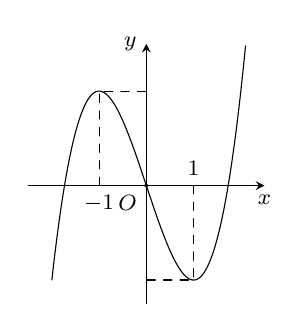
\begin{tikzpicture}[>=stealth, scale=0.6, font=\footnotesize, line join=round, line cap=round]
			\def \xmin{-2.5}
			\def \xmax{2.5}
			\def \ymin{-2.5}
			\def \ymax{3}
			\draw[->] (\xmin,0)--(\xmax,0) node[below] {$x$};
			\draw[->] (0,\ymin)--(0,\ymax) node[left] {$y$};
			\draw[smooth,samples=200,domain=-2.0:2.1] plot (\x,{(\x)^3-3*(\x)});
			\draw[fill=black] (0,0) node[below left=-0.1] {$O$} circle (1pt);
			\node at (1,0) [above] {$1$};
			\node at (-1,0) [below] {$-1$};
			\draw[dashed] (-1,0)--(-1,2)--(0,2);
			\draw[dashed] (1,0)--(1,-2)--(0,-2);
		\end{tikzpicture}
	}
	\loigiai{
		Dựa vào đồ thị hàm số, ta thấy
		\begin{itemize}
			\item Đồ thị có hình dạng của hàm số bậc ba $y=ax^3+bx^2+cx+d$ với $a>0$.
			\item Đồ thị hàm số đi qua gốc tọa độ $O(0;0)$, suy ra $d=0$.
			\item Đồ thị hàm số đạt cực trị tại các điểm có hoành độ $x=1$ và $x=-1$.
		\end{itemize}
		Xét các hàm số ở các phương án
		\begin{itemize}
			\item Hàm số $y=x^3+2x+1$ có $d=1$ (loại)
			\item Hàm số $y=-x^3+3x$ có $a=-1<0$ (loại).
			\item Hàm số $y=x^3+3x^2$ đi qua $O(0;0)$, đạo hàm $y'=3x^2+6x=0 \Leftrightarrow \hoac{&x=0\\&x=-2}$ (loại).
			\item Hàm số $y=x^3-3x$ đi qua $O(0;0)$, có $a=1>0$, đạo hàm $y'=3x^2-3=0 \Leftrightarrow x=\pm 1$ (thỏa mãn).
		\end{itemize}
		Vậy đồ thị đã cho là của hàm số $y=x^3-3x$.
	}
\end{ex}

\begin{ex}%[2D1H5-1]%[Dự án đề TT Toán NH25-26-Dot 3- Bùi Lương Phúc]%[Cụm 13-Hải Phòng]%[GVPB - Viet Hoang Pham]
\immini[thm]{
Tìm hệ số $a$, $b$, $c$ để hàm số $y=\dfrac{ax+2}{cx+b}$ có đồ thị như hình vẽ bên
\choice
{$a=2$, $b=2$, $c=-1$}
{$a=1$, $b=2$, $c=1$}
{$a=1$, $b=1$, $c=-1$}
{\True $a=1$, $b=-2$, $c=1$}
}{
\begin{tikzpicture}[scale=0.7,line cap=round,line join=round,font=\footnotesize,>=stealth]
\draw[->] (-3,0)--(7,0) node[below right]{$x$};
\draw[->] (0,-3)--(0,5) node[above left]{$y$};
\node[below left] at (0,0){$O$};
\foreach \x in {-2,2}\node[below left] at (\x,0){$\x$};
\foreach \y in {-1,1}\node[below left] at (0,\y){$\y$};
\draw[dashed] (2,-3)--(2,5) (-3,1)--(7,1);
\draw[smooth,domain=3:7] plot(\x,{(\x+2)/(\x-2)});
\draw[smooth,domain=-3:1] plot(\x,{(\x+2)/(\x-2)});
\fill (0,0) circle(1pt) (0,0) circle(1pt) (-2,0) circle(1pt) (2,0) circle(1pt) (0,1) circle(1pt)(0,-1) circle(1pt);
\end{tikzpicture}
}
\loigiai{
Từ phương trình $y=\dfrac{ax+2}{cx+b}$ cùng với đồ thị hàm số ta có:
\begin{itemize}
\item Đồ thị hàm số có tiệm cận đứng $x=-\dfrac{b}{c}=2\Rightarrow b=-2c$\quad $(1)$.
\item Đồ thị hàm số có tiệm cận ngang $y=\dfrac{a}{c}=1\Rightarrow a=c$\quad $(2)$.
\item Vì đồ thị hàm số đi qua điểm $(0;-1)$ nên $-1=\dfrac{a\cdot 0+2}{c\cdot 0+b}\Rightarrow \dfrac{2}{b}=-1\Rightarrow b=-2$\quad $(3)$.
\end{itemize}
Từ $(1)$, $(2)$ và $(3)$ suy ra $a=1$, $b=-2$, $c=1$.
}
\end{ex}

\begin{ex}%[2D1H5-1]%[Dự án C đề thi thử TN Môn Toán NH25-26 - Dot 4 - Bui Luong Phuc]%[THPT Lê Thánh Tông-TPHCM]%[GVPB - Viet Hoang Pham]
\immini[thm]{
Tìm hệ số $b$, $c$ để hàm số $y = \dfrac{2}{cx+b}$ có đồ thị như hình vẽ bên
\choice[2]
{$\heva{&b=2 \\ &c=-1 }$}
{$\heva{&b=1 \\ &c=-1 }$}
{$\heva{&b=2 \\ &c=1 }$}
{\True $\heva{& b=-2 \\ &c=1 }$}
}{
\begin{tikzpicture}[>=stealth, font=\footnotesize, line cap=round, line join=round, scale=0.6]
\def\xmin{-2} \def\xmax{6} \def\ymin{-3} \def\ymax{3}
\def\f{2/(\x-2)}
\draw[->] (\xmin,0) -- (\xmax,0) node[below] {$x$};
\draw[->] (0,\ymin) -- (0,\ymax) node[left] {$y$};
\draw (2,\ymin) -- (2,\ymax);
\begin{scope}
\clip (\xmin,\ymin) rectangle (\xmax,\ymax);
\draw[smooth, samples=100, domain=\xmin:1.4] plot (\x, {\f});
\draw[smooth, samples=100, domain=2.6:\xmax] plot (\x, {\f});
\end{scope}
\foreach \p/\ang/\lbl in {(0,0)/135/O, (2,0)/-45/2, (0,-1)/210/-1}
\fill \p circle (1pt) node[shift={(\ang:0.3)}] {$\lbl$};
\end{tikzpicture}
}
\loigiai{
Đồ thị hàm số $y = \dfrac{2}{cx+b}$ cắt trục tung tại điểm $(0;-1)$, có tiệm cận đứng $x = 2$ suy ra
\[\heva{&-1 = \dfrac{2}{c \cdot 0 + b}\\& c\cdot 2 + b = 0}\Leftrightarrow \heva{&b = -2\\& c = 1.}
\]
Vậy $b = -2$, $c = 1$.
}
\end{ex}

\begin{ex}%[2D1H5-1]%[Dự án C đề thi thử TN Môn Toán NH25-26 - Dot 4 - Sỹ Trường]%[THPT Nguyễn Trãi - Hà Nội]%[GVPB - Khắc Thiên]
	\immini[thm]
	{
		Hình vẽ bên là đồ thị của hàm số nào trong các hàm số dưới đây?
		\choice
		{$y=x^3+2x+1$}
		{\True $y=x^3-2x+1$}
		{$y=-x^3+2x+1$}
		{$y=x^3-2x^2+1$}
	}
	{
		\begin{tikzpicture}[line join=round, line cap=round,>=stealth]
			\tikzset{every node/.style={scale=0.9}}
			\draw[->] (-2.1,0)--(2.1,0) node[below] {$x$};
			\draw[->] (0,-1.1)--(0,2.6) node[left] {$y$};
			\draw (0,0) node [below left] {$O$};
			\foreach \y/\ny in {1/1}
			\draw (1pt,\y)--(-1pt,\y) node [left] {$\ny$};
			\begin{scope}
				\clip (-2,-1) rectangle (2,2.5);
				\draw[samples=200,domain=-2:2,smooth,variable=\x] plot (\x,{1*((\x)^3)+0*((\x)^2)+-2*(\x)+1});
			\end{scope}
		\end{tikzpicture}
	}
	\loigiai{
		Từ đồ thị suy ra:
		\begin{itemize}
			\item Đồ thị có nét cuối hướng lên nên hệ số của $x^3$ phải là số dương.
			\item Hàm số có hai điểm cực trị (hàm số $y=x^3+2x+1$ đồng biến trên $\mathbb{R}$ do có $y'=3x^2+2>0$, $\forall x \in \mathbb{R}$ nên bị loại).
			\item Hàm số không có điểm cực trị $x=0$ (hàm số $y=x^3-2x^2+1$ có điểm cực trị $x=0$ do có $y'=3x^2-4x=x(3x-4)$ nên bị loại).
		\end{itemize}
		Vậy hàm số cần tìm là $y=x^3-2x+1$.
	}
\end{ex}

\begin{ex}%[2D1H5-1]%[Dự án đề TT Toán NH25-26-Dot 3-PhucChuong]%[THPT Trần Nhân Tông - Hà Nội]%[GVPB - Phan Quốc Trí]
	\immini[thm]{Cho hàm số $y=\dfrac{ax+b}{cx+d}$ $(ac \neq 0, ad-bc \neq 0)$ có đồ thị như hình vẽ bên. Trong các hệ số $a$, $b$, $c$, $d$ có bao nhiêu số dương?
		\choice
		{\True $2$}
		{$1$}
		{$3$}
		{$0$}}{\begin{tikzpicture}[scale=.7, font=\footnotesize, line join=round, line cap=round, >=stealth]
			\fill (0,0)node[below left]{$O$} circle (1pt)
			(1,0)node[above left]{$1$} circle (1pt)
			(0,-1)node[below left]{$-1$} circle (1pt)
			(2,0)node[above right]{$2$} circle (1pt)
			(0,-2)node[below left]{$-2$} circle (1pt);
			\draw[->] (-3,0)--(6,0)node[above]{$x$};
			\draw[->] (0,-4)--(0,4)node[left]{$y$};
			\draw[smooth,samples=100,domain=-3:0.667]
			plot(\x,{-1+1/(\x-1)});
			\draw[smooth,samples=100,domain=1.2:6]
			plot(\x,{-1+1/(\x-1)});
			\draw[dashed] (1,-4)--(1,4) (-3,-1)--(6,-1);
	\end{tikzpicture}}
	\loigiai{Đồ thị hàm số có đường tiệm cận đứng là $x=1$, do đó $-\dfrac{d}{c}=1$.\\
		Đồ thị hàm số có đường tiệm cận ngang là $y=-1$, do đó $\dfrac{a}{c}=-1$\\
		Đồ thị hàm số đi qua điểm $(2;0)$ nên $2a+b=0$.\\
		Đồ thị hàm số đi qua điểm $(0;-2)$ nên $\dfrac{b}{d}=-2$.\\
		Như vậy $\heva{&\dfrac{d}{c}<0 \\ &\dfrac{a}{c}<0 \\& \dfrac{b}{d}<0}$ hay $\heva{&\text{$a$ và $d$ cùng dấu (vì cùng khác dấu với $c$)}\\&\text{$b$ và $c$ cùng dấu}\\&\text{$a$ và $c$ trái dấu.}}$\\
		
		Vậy trong $4$ số $a$, $b$, $c$ và $d$ có hai số dương, hai số âm.}
\end{ex}

\begin{ex}%[2D1N1-2]%[Dự án C đề thi thử TN Môn Toán NH25-26 - Đợt 4 - Đỗ Minh Phúc]%[Lần 1 Liên trường Hà Nội]%[GVPB - Lê Phúc]
	Cho hàm số $y=f(x)$ liên tục trên $\mathbb{R}$ và có bảng xét dấu đạo hàm như sau
	\begin{center}
		
\begin{tikzpicture}
			\tkzTabInit[nocadre=false, lgt=1.2, espcl=2.5, deltacl=0.5]
			{$x$/0.7,$f’(x)$/0.7}
			{$-\infty$,$-3$,$0$,$2$,$+\infty$}
			\tkzTabLine{,+,0,-,0,+,0,-,}
		\end{tikzpicture}
	\end{center}
	Hàm số $y=f(x)$ đồng biến trên khoảng nào trong các khoảng sau đây?
	\choice
	{\True $(0;1)$}
	{$(-3;0)$}
	{$(2;+\infty)$}
	{$(-\infty ;-1)$}
	\loigiai{
		Dựa vào bảng biến thiên ta có hàm số $y=f(x)$ đồng biến trên khoảng $(0;1)$.
	}
\end{ex}

\begin{ex}%[2D1N1-2]%[Dự án đề thi thử đợt 3-GV Ngô Tất Thành]%[SGD tỉnh Lạng Sơn]%[GVPB - ThanhTa]
	Cho hàm số $y=f(x)$ có đồ thị như bên dưới.
	\begin{center}
		\begin{tikzpicture}[scale=0.8, font=\footnotesize, line join=round, line cap=round, >=stealth]
			\draw[->] (-3,0) -- (3.5,0) node[below] {$x$};
			\draw[->] (0,-3) -- (0,3.5) node[left] {$y$};
			\node[above left] at (0,0) {$O$};
			\draw[thick,samples=100,domain=0.35:3.2] plot (\x,{\x+1/(\x)});
			\draw[thick,samples=100,domain=-3.2:-0.35] plot (\x,{\x+1/(\x)});
			\draw[dashed] (-3,-3) -- (3,3);
			\draw[dashed] (1,0) node[below] {$1$} -- (1,2) -- (0,2) node[left] {$2$};
			\draw[dashed] (-1,0) node[above] {$-1$} -- (-1,-2) -- (0,-2) node[right] {$-2$};
			\draw [fill=black] (1,2) circle (1pt);
			\draw [fill=black] (-1,-2) circle (1pt);
		\end{tikzpicture}
	\end{center}
	Hàm số đã cho nghịch biến trên khoảng nào trong các khoảng sau đây?
	\choice
	{$(0;2)$}
	{$(-1;1)$}
	{\True $(-1;0)$}
	{$(1;2)$}
	\loigiai{
		Dựa vào đồ thị, ta thấy trên khoảng $(-1;0)$, đồ thị hàm số có hướng đi xuống từ trái sang phải.
		Vậy hàm số nghịch biến trên khoảng $(-1;0)$.
	}
\end{ex}

\begin{ex}%[2D1N1-2]%[Dự án C đợt 3 NH25-26- Nguyễn Hữu Đức]%[SỞ GIÁO DỤC - TUYÊN QUANG]%[GVPB: Thanh Phát]
	Cho hàm số $y = f(x)$ có bảng biến thiên như sau
	\begin{center}
		
\begin{tikzpicture}
			\tkzTabInit[lgt=1.5, espcl=3]
			{$x$ /1, $y'$ /0.7, $y$ /2.5}
			{$-\infty$, $-1$, $3$, $+\infty$}
			\tkzTabLine{, +, 0, -, 0, +, }
			\tkzTabVar{-/ $-\infty$, +/ $6$, -/ $-26$, +/ $+\infty$}
		\end{tikzpicture}
	\end{center}
	Hàm số đã cho nghịch biến trên khoảng nào sau đây?  
	\choice
	{$(-26; 6)$}  
	{$(-\infty; -1)$}  
	{$(3; +\infty)$}  
	{\True $(-1; 2)$}  
	\loigiai{
		Dựa vào bảng biến thiên, đạo hàm $y' < 0$ trên khoảng $(-1; 3)$.\\  
		Do đó hàm số nghịch biến trên khoảng $(-1; 3)$, suy ra nghịch biến trên $(-1; 2)$ vì $(-1; 2) \subset (-1; 3)$.
	}
\end{ex}

\begin{ex}%[2D1N1-2]%[Dự án C đề thi thử TN Môn Toán NH25-26 - Dot 4 - Bui Luong Phuc]%[THPT Lê Thánh Tông-TPHCM]%[GVPB - Viet Hoang Pham]
\immini[thm]{
Cho hàm số $y=f(x)$ có đồ thị như hình vẽ bên.
Hàm số đã cho đồng biến trên khoảng nào trong các khoảng sau đây?
\choice[2]
{$(-\infty;1)$}
{$(1;2)$}
{\True $(2;+\infty)$}
{$(-1;1)$}
}{
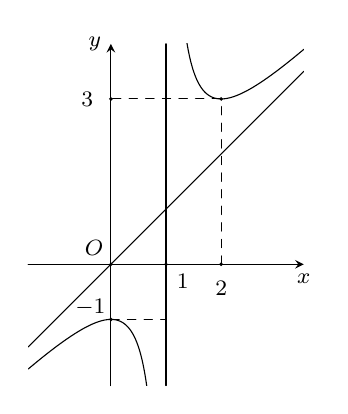
\begin{tikzpicture}[>=stealth, font=\footnotesize, line cap=round, line join=round,scale=0.7]
\def\xmin{-1.5} \def\xmax{3.5} \def\ymin{-2.2} \def\ymax{4}
\def\f{((\x)^2-\x+1)/(\x-1)}
\draw[->] (\xmin,0) -- (\xmax,0) node[below] {$x$};
\draw[->] (0,\ymin) -- (0,\ymax) node[left] {$y$};
\draw (1,\ymin) -- (1,\ymax) ;
\draw[dashed] (2,0) |- (0,3) (0,-1) -| (1,0);
\begin{scope}
\clip (\xmin,\ymin) rectangle (\xmax,\ymax);
\draw[smooth, samples=100, domain=\xmin:0.85] plot (\x, {\f});
\draw[smooth, samples=100, domain=1.15:\xmax] plot (\x, {\f});
\draw (\xmin,\xmin) -- (\xmax,\xmax);
\end{scope}
\foreach \p/\ang/\lbl in {(0,0)/135/O, (1,0)/-45/1, (2,0)/-90/2, (0,-1)/150/-1, (2,3)/-135/ , (0,3)/180/3}
\fill \p circle (1pt) node[shift={(\ang:0.3)}] {$\lbl$};
\end{tikzpicture}
}
\loigiai{
Dựa vào đồ thị, ta thấy trên khoảng $(2;+\infty)$, đồ thị hàm số đi lên từ trái sang phải.\\
Vậy hàm số đã cho đồng biến trên khoảng $(2;+\infty)$.
}
\end{ex}

\begin{ex}%[2D1N1-2]%[TT-THPT Lê Thánh Tông-TPHCM-L2-NH25-26]%[Bùi Quang Phú]%[PB: Phan Anh]
	Cho hàm số $y=f(x)$ có bảng biến thiên như sau:
	\begin{center}
		
\begin{tikzpicture}
			\tikzset{double style/.append style={double distance=1.5pt}}
			\tkzTabInit[nocadre=false,lgt=1.2,espcl=2.5,deltacl=0.6]
			{$x$/0.6,$f'(x)$/0.6,$f(x)$/2}
			{$-\infty$,$-1$,$1$,$+\infty$}
			\tkzTabLine{,+,$0$,-,$0$,+,}
			\tkzTabVar{-/$-\infty$,+/$2$,-/$-2$,+/$+\infty$}
		\end{tikzpicture}
	\end{center}
	Hàm số đã cho nghịch biến trên khoảng nào dưới đây?
	\choice
	{$(-2;2)$}
	{\True $(-1;1)$}
	{$(-2;1)$}
	{$(1;+\infty)$}
	\loigiai{
		Dựa vào bảng biến thiên, hàm số đã cho nghịch biến trên khoảng $(-1;1)$.
	}
\end{ex}

\begin{ex}%[2D1N1-2]%[Dự án C đề thi thử TN Môn Toán NH25-26 - Dot 4 - Hồng Trường Sơn]%[THPT Mai Anh Tuấn - Thanh Hóa]%[GVPB - Lê Hữu Kiệt]
	Cho hàm số $f(x)$ có bảng biến thiên như sau
	\begin{center}
		
\begin{tikzpicture}
			\tkzTabInit[nocadre=false,lgt=1.5,espcl=2.5,deltacl=.5]
			{$x$ /.7, $f’(x)$ /.7,$f(x)$ /2}
			{$-\infty$ , $-1$ , $0$ , $1$ , $+\infty$}
			\tkzTabLine{ ,-,0,+,0,-,0,+, }
			\tkzTabVar{+/$+\infty$ ,-/ $-1$ ,+/$4$, -/$-1$,+/$+\infty$}
		\end{tikzpicture}
	\end{center}
	Hàm số đã cho đồng biến trên khoảng nào dưới đây?
	\choice
	{\True $(-1;0)$}
	{$(-\infty ;-1)$}
	{$(-1;1)$}
	{$(0;1)$}
	\loigiai{
		Từ bảng biến thiên ta có $f'(x)>0$, $\forall x\in (-1;0)\cup (1;+\infty)$.\\
		Do đó, hàm số đồng biến trên các khoảng $(-1 ; 0)$ và $(1;+\infty)$.
	}
\end{ex}

\begin{ex}%[2D1N1-2]%[Dự án C đề thi thử TN Môn Toán NH25-26 - Dot 4 - Sỹ Trường]%[THPT Nguyễn Trãi - Hà Nội]%[GVPB - Khắc Thiên]
	Cho hàm số $y=f(x)$ có bảng xét dấu đạo hàm như sau:
	\begin{center}
		
\begin{tikzpicture}
			\tkzTabInit[deltacl=0.5,espcl=2.5,lgt=2]
			{$x$/1,$y'$/1}
			{$-\infty$,$1$,$2$,$3$,$4$,$+\infty$}
			\tkzTabLine{,-,0,+,0,+,0,-,0,+,}
		\end{tikzpicture}
	\end{center}
	Hàm số đã cho nghịch biến trên khoảng nào dưới đây?
	\choice
	{$(-\infty;2)$}
	{\True $(3;4)$}
	{$(4;+\infty)$}
	{$(1;3)$}
	\loigiai{
		Dựa vào bảng xét dấu đạo hàm ta thấy $f'(x)<0 \Leftrightarrow x \in(-\infty;1) \cup(3;4)$.\\
		Do đó hàm số đã cho nghịch biến trên khoảng $(-\infty;1)$ và $(3;4)$.
	}
\end{ex}

\begin{ex}%[2D1N1-2]%[Dự án C đề thi thử TN Môn Toán NH25-26 - Dot 4 - Sỹ Trường]%[THPT Nguyễn Trãi - Hà Nội]%[GVPB - Khắc Thiên]
	\immini[thm]
	{
		Cho hàm số $y=f(x)$ có đồ thị như hình bên. Hàm số đã cho đồng biến trên khoảng nào dưới đây?
		\choice
		{$(0;2)$}
		{$(0;+\infty)$}
		{\True $(2;+\infty)$}
		{$(-\infty;2)$}
	}
	{
		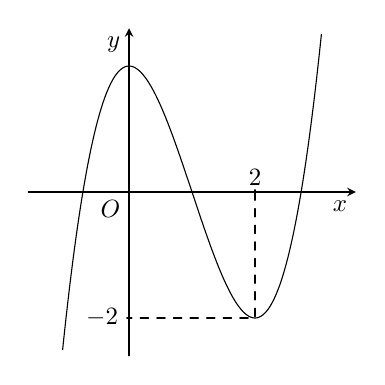
\begin{tikzpicture}[line join=round, line cap=round,>=stealth,scale=0.8]
			\tikzset{every node/.style={scale=0.9}}
			\draw[->] (-1.6,0)--(3.6,0) node[below left] {$x$};
			\draw[->] (0,-2.6)--(0,2.6) node[below left] {$y$};
			\draw (0,0) node [below left] {$O$};
			\foreach \x/\nx in {2/2}
			\draw (\x,1pt)--(\x,-1pt) node [above] {$\nx$};
			\foreach \y/\ny in {-2/-2}
			\draw (1pt,\y)--(-1pt,\y) node [left] {$\ny$};
			\draw[dashed](2,0)--(2,-2)--(0,-2);
			\begin{scope}
				\clip (-1.5,-2.5) rectangle (3.5,2.5);
				\draw[samples=200,domain=-1.5:3.5,smooth,variable=\x] plot (\x,{1*((\x)^3)+-3*((\x)^2)+0*(\x)+2});
			\end{scope}
		\end{tikzpicture}
	}
	\loigiai{
		Dựa vào đồ thị hàm số đã cho, ta thấy hàm số đồng biến (đồ thị đi lên) trên khoảng $(2;+\infty)$ và $(-\infty;0)$.
	}
\end{ex}

\begin{ex}%[2D1N2-1]%[Dự án đề thi thử NH25-26]%[THPT Chuyên Phan Bội Châu - Nghệ An]%[GVPB2 Khắc Thiên]
	Cho hàm số $y=f(x)$ có đạo hàm $f'(x) = (x-1)(x-2)^2(x-3)^3$. Số điểm cực trị của hàm số $y=f(x)$ là
	\choice
	{$1$}
	{\True $2$}
	{$3$}
	{$0$}
	\loigiai{
		Xét phương trình $f'(x) = 0 \Leftrightarrow \hoac{&x=1 \\ &x=2 \\ &x=3.}$\\
		Ta thấy $x=1$ và $x=3$ là các nghiệm bội lẻ, $x=2$ là nghiệm bội chẵn.\\
		Do $f'(x)$ chỉ đổi dấu khi đi qua các nghiệm bội lẻ nên hàm số $y=f(x)$ có $2$ điểm cực trị.
	}
\end{ex}

\begin{ex}%[2D1N2-1]%[Dự án C đề thi thử TN Môn Toán NH25-26 - Dot 4 - Sỹ Trường]%[THPT Nguyễn Trãi - Hà Nội]%[GVPB - Khắc Thiên]
	Cho hàm số $y=f(x)$ liên tục trên $\mathbb{R}$ và có bảng xét dấu của đạo hàm như sau:
	\begin{center}
		
\begin{tikzpicture}
			\tkzTabInit[deltacl=0.5,espcl=2.5,lgt=2]
			{$x$/1,$y'$/1}
			{$-\infty$,$-3$,$-2$,$3$,$5$,$+\infty$}
			\tkzTabLine{,-,0,+,0,-,0,+,0,-,}
		\end{tikzpicture}
	\end{center}
	Số điểm cực trị của hàm số đã cho là
	\choice
	{$3$}
	{\True $4$}
	{$2$}
	{$5$}
	\loigiai{
		Từ bảng xét dấu suy ra hàm số $y=f(x)$ có $4$ lần đổi dấu qua các nghiệm của đạo hàm, do đó hàm số có $4$ điểm cực trị.
	}
\end{ex}

\begin{ex}%[2D1N3-1]%[Dự án C đề thi thử TN Môn Toán NH25-26 - Dot 4 - Sỹ Trường]%[THPT Nguyễn Trãi - Hà Nội]%[GVPB - Khắc Thiên]
	\immini[thm]
	{
		Cho hàm số $y=f(x)$ liên tục và có đồ thị trên đoạn $[-2;2]$ như hình vẽ bên. Gọi $M$ và $m$ lần lượt là giá trị lớn nhất và giá trị nhỏ nhất của hàm số $f(x)$ trên đoạn $[-2;2]$. Khi đó, giá trị của biểu thức $M-m$ bằng
		\choice
		{\True $5$}
		{$-4$}
		{$0$}
		{$3$}
	}
	{
		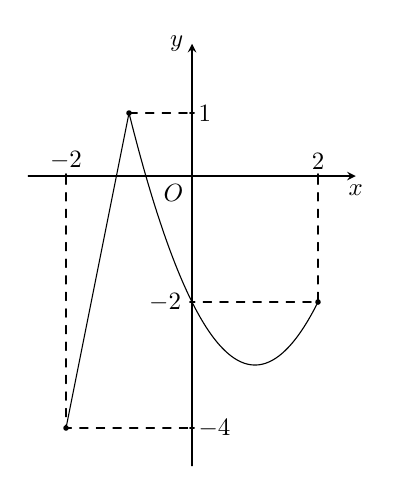
\begin{tikzpicture}[line join=round, line cap=round,>=stealth,scale=0.8]
			\tikzset{every node/.style={scale=0.9}}
			\draw[->] (-2.6,0)--(2.6,0) node[below] {$x$};
			\draw[->] (0,-4.6)--(0,2.1) node[left] {$y$};
			\draw (0,0) node [below left] {$O$};
			\foreach \x/\nx in {-2/-2,2/2}
			\draw (\x,1pt)--(\x,-1pt) node [above] {$\nx$};
			\foreach \y/\ny in {-2/-2}
			\draw (1pt,\y)--(-1pt,\y) node [left] {$\ny$};
			\foreach \y/\ny in {1/1,-4/-4}
			\draw (1pt,\y)--(-1pt,\y) node [right] {$\ny$};
			\draw[dashed](-2,0)--(-2,-4)--(0,-4);
			\draw[dashed](2,0)--(2,-2)--(0,-2);
			\draw[dashed](-1,1)--(0,1);
			\draw[fill=black](-1,1) circle(1pt) (-2,-4) circle(1pt) (2,-2) circle(1pt);
			\begin{scope}
				\clip (-2.5,-4.5) rectangle (2.5,2);
				\draw[samples=200,domain=-2:-1,smooth,variable=\x] plot (\x,{5*(\x)+6});
				\draw[samples=200,domain=-1:2,smooth,variable=\x] plot (\x,{(\x)^2-2*(\x)-2});
			\end{scope}
		\end{tikzpicture}
	}
	\loigiai{
		Xét trên đoạn $[-2;2]$:\\
		Điểm cao nhất của đồ thị có tung độ là $1$. Vậy giá trị lớn nhất là $M=1$.\\
		Điểm thấp nhất của đồ thị có tung độ là $-4$ (tại $x=-2$). Vậy giá trị nhỏ nhất là $m=-4$.\\
		Do đó $M-m=1-(-4)=5$.
	}
\end{ex}

\begin{ex}%[TT Cụm 5 - Ninh Bình-NH25-26]%[Nguyễn Chiến]%[Phản biện 1: Nguyễn Tấn Tài]%[2D1N4-1]
	Số đường tiệm cận của đồ thị hàm số $y=2x+3+\dfrac{1}{x-1}$ là
	\choice
	{$0$}
	{$3$}
	{$1$}
	{\True $2$}
	\loigiai{
		Ta có $\lim\limits_{x\to \pm\infty}\left[y-(2x+3)\right]=\lim\limits_{x\to \pm\infty}\left(\dfrac{1}{x-1}\right)=0\Rightarrow y=2x+3$ là đường tiệm cận xiên của đồ thị hàm số.\\
		$\lim\limits_{x\to 1^+}y=\lim\limits_{x\to 1^+}\left(2x+3+\dfrac{1}{x-1}\right)=+\infty\Rightarrow x=1$ là đường tiệm cận đứng của đồ thị hàm số.
	}
\end{ex}

\begin{ex}%[2D1N4-1]%[Dự án C đề thi thử TN Môn Toán NH25-26 - Dot 4 - Thy Nguyen Vo Diem]%[Liên trường THPT cụm 09 - Đợt 2 - Hà Nội]%[GVPB - Thanh Phát]
	Cho hàm số $y = f(x)$ có bảng biến thiên như sau
	\begin{center}
		
\begin{tikzpicture}
			\tkzTabInit[nocadre=false,lgt=1.2,espcl=3]{$x$ / 0.6, $f'(x)$ / 0.6, $f(x)$ / 2}
			{$-\infty$, $1$, $+\infty$}
			\tkzTabLine{ , -, d, -, }
			\tkzTabVar{+/ $0$, -D+/ $-\infty$ / $+\infty$, -/ $0$}
		\end{tikzpicture}
	\end{center}
	Tiệm cận ngang của đồ thị hàm số $y = f(x)$ có phương trình là
	\choice
	{$x=1$}
	{\True $y=0$}
	{$y=1$}
	{$x=0$}
	\loigiai{
		Dựa vào bảng biến thiên, ta thấy 
		$$\lim\limits_{x \to -\infty} f(x) = 0 \quad \text{và} \quad \lim\limits_{x \to +\infty} f(x) = 0.$$
		Do đó, đồ thị hàm số $y = f(x)$ có tiệm cận ngang là đường thẳng $y = 0$.
	}
\end{ex}

\begin{ex}%[2D1N4-1]%[Dự án đề TT Toán NH25-26-Dot 3- Bùi Lương Phúc]%[Cụm 13-Hải Phòng]%[GVPB - Viet Hoang Pham]
Cho hàm số $y=f(x)$ có bảng biến thiên như hình dưới đây.
\begin{center}

\begin{tikzpicture}
\tkzTabInit[nocadre=true, lgt=1.3,espcl=2.5]
{$x$/1,$y'$/1,$y$/2}
{$-\infty$,0,1,$+\infty$}
\tkzTabLine{,-,d,-,0,+}
\tkzTabVar
{+/ $2$ , -D+/ $-4$ / $+\infty$ , -/ $-2$ , +/ $+\infty$}
\end{tikzpicture}
\end{center}
Số đường tiệm cận ngang của đồ thị hàm số đã cho là
\choice
{$3$}
{\True $1$}
{$2$}
{$0$}
\loigiai{
Vì $\lim\limits_{x\to-\infty}f(x)=2$ và $\lim\limits_{x\to+\infty}f(x)=+\infty$ nên $y=2$ là tiệm cận ngang duy nhất.\\
Vậy đồ thị hàm số $y=f(x)$ có đúng một tiệm cận ngang.
%%hàm f(x) tồn tại, ví dụ f(x) = 2 + 1 / x - 5 / (x² + 1).%%
}
\end{ex}

\begin{ex}%[2D1N4-1]%[Dự án đề thi thử NH25-26]%[THPT Chuyên Phan Bội Châu - Nghệ An]%[GVPB2 Khắc Thiên]
	Đường tiệm cận ngang đồ thị hàm số $y=\dfrac{3x-1}{x-2}$ là
	\choice
	{$x=2$}
	{$y=2$}
	{$x=3$}
	{\True $y=3$}
	\loigiai{
		Ta có $\lim\limits_{x \to \pm\infty} \dfrac{3x-1}{x-2} = 3$.\\
		Vậy đường thẳng $y=3$ là tiệm cận ngang của đồ thị hàm số.
	}
\end{ex}

\begin{ex}%[2D1N4-1]%[Dự án C đề thi thử TN Môn Toán NH25-26 - Đợt 4 - Đỗ Minh Phúc]%[Lần 1 Liên trường Hà Nội]%[GVPB - Lê Phúc]
	Đồ thị hàm số $y=\dfrac{2 x+1}{2-x}$ có đường tiệm cận ngang là đường thẳng có phương trình
	\choice
	{\True $y=-2$}
	{$x=-2$}
	{$y=1$}
	{$x=2$}
	\loigiai{
		Ta có $\lim\limits_{x \rightarrow+\infty} \dfrac{2 x+1}{2-x}=\lim\limits_{x \rightarrow+\infty} \dfrac{2+\frac{1}{x}}{\frac{2}{x}-1}=-2$ và $\lim\limits_{x \rightarrow-\infty} \dfrac{2 x+1}{2-x}=\lim\limits_{x \rightarrow-\infty} \dfrac{2+\frac{1}{x}}{\frac{2}{x}-1}=-2$.\\
		Vậy đường thẳng $y=-2$ là đường tiệm cận ngang của đồ thị hàm số $y=\dfrac{2 x+1}{2-x}$.
	}
\end{ex}

\begin{ex}%[Dự án C - Đợt 3 - Sở Giáo Dục Sơn La]%[GV biên soạn: Nhật Thiện - GV phản biện: Nguyễn Tiến]%[2D1N4-1]
	Tiệm cận đứng của đồ thị hàm số $y=\dfrac{2x-1}{x-1}$ là đường thẳng có phương trình
	\choice
	{$y=1$}
	{\True $x=1$}
	{$y=2$}
	{$x=2$}
	\loigiai{
		Ta có $\lim\limits_{x\to 1^\pm} y=\pm \infty$. \\
		Suy ra phương trình tiệm cận đứng của đồ thị hàm số là $x=1$.
	}
\end{ex}

\begin{ex}%[Đề thi thử môn Toán THPT Cổ Loa, năm học 2025-2026]%[Đỗ Minh Phúc-Lê Phúc]%[2D1N4-1]
	\immini[thm]{Cho hàm số $y=\dfrac{ax+b}{cx+d}$ ($ac \neq 0$, $ad-bc \neq 0$) có đồ thị như hình vẽ. Đường tiệm cận ngang của đồ thị hàm số đã cho có phương trình là
	\choice
	{$y=1$}
	{\True $y=-1$}
	{$x=1$}
	{$x=-1$}}
	{	\begin{tikzpicture}[line join = round, line cap = round,>=stealth,font=\footnotesize,scale=.65,declare function={f(\x)=(\a*\x+(\b))/(\c*\x+(\d));}]
			\def\xt{-5} \def\xp{4} \def\yd{-4} \def\yt{3}
			\def\a{-1}
			\def\b{1}
			\def\c{1}
			\def\d{1}
			\draw[->] (\xt,0)--(\xp,0) node[below]{$x$};
			\draw[->] (0,\yd)--(0,\yt) node[right]{$y$};
			\fill (0,0) circle (1pt) node[above left]{$O$};
			\begin{scope}
				\clip (\xt+0.1,\yd+0.1) rectangle (\xp-0.1,\yt-0.1);
				\pgfmathsetmacro{\tcn}{(\a)/(\c)}
				\pgfmathsetmacro{\tcd}{-(\d)/(\c)}
				\draw (\xt,\tcn)--(\xp,\tcn) (\tcd,\yd)--(\tcd,\yt);
				\draw[samples=150,smooth,domain={\tcd+0.01}:\xp] plot(\x,{f(\x)});
				\draw[samples=150,smooth,domain=\xt:{\tcd-0.01}] plot(\x,{f(\x)});
			\end{scope}
			\fill (0,-1) circle (1pt) node [below right]{$-1$};
			\fill (-1,0) circle (1pt) node [above left]{$-1$};
	\end{tikzpicture}}
	\loigiai{
		Dựa vào đồ thị của hàm số như hình vẽ, ta có đường tiệm cận ngang của đồ thị hàm số là đường thẳng $y=-1$.
	}
\end{ex}

\begin{ex}%[2D1N4-1]%[Đề thi thử môn Toán TRƯỜNG THPT Hàm Rồng năm học 2025-2026]%[Dương Phạm - GVPB2 Đỗ Minh Vũ]
	Phương trình đường tiệm cận ngang của đồ thị hàm số $y = \dfrac{x-3}{5x-16}$ là
	\choice
	{$y = \dfrac{16}{5}$}
	{$x = \dfrac{16}{5}$}
	{$x = \dfrac{1}{5}$}
	{\True $y = \dfrac{1}{5}$}
	\loigiai{
		Ta có: $\lim\limits_{x \to -\infty} \dfrac{x-3}{5x-16} = \dfrac{1}{5}$ và $\lim\limits_{x \to +\infty} \dfrac{x-3}{5x-16} = \dfrac{1}{5}$.\\
		Phương trình đường tiệm cận ngang của đồ thị hàm số $y = \dfrac{x-3}{5x-16}$ là $y = \dfrac{1}{5}$.
	}
\end{ex}

\begin{ex}%[2D1N4-1]%[Dự án đề TT Toán NH25-26-Dot 3-PhucChuong]%[THPT Lê Quý Đôn - Đống Đa - Hà Nội]%[GVPB - Phan Quốc Trí]
 	\immini[thm]{Cho đồ thị hàm số như hình vẽ bên dưới. Đường tiệm cận ngang của đồ thị hàm số là
 		\choice
 		{$x=2$}
 		{$y=2$}
 		{$x=1$}
 		{\True $y=1$}}
 	{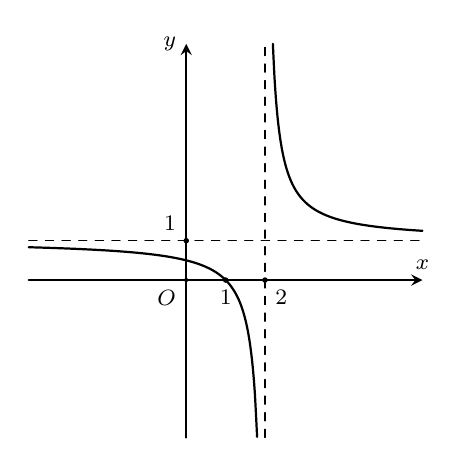
\begin{tikzpicture}[scale=.5, font=\footnotesize, line join=round, line cap=round, >=stealth, thick]
 			\draw[->] (-4,0)--(6,0)node[above]{$x$};
 			\draw[->] (0,-4)--(0,6)node[left]{$y$};
 			\draw[smooth,samples=100,domain=-4:1.8] 
 			plot(\x,{1+1/(\x-2)});
 			\draw[smooth,samples=100,domain=2.2:6] 
 			plot(\x,{1+1/(\x-2)});
 			\draw[dashed, thin] (2,-4)--(2,6)
 			(-4,1)--(6,1);
 			\fill (0,0)node[below left]{$O$} circle (1.5pt)
 			(1,0)node[below]{$1$} circle (2pt)
 			(0,1)node[above left]{$1$} circle (2pt)
 			(2,0)node[below right]{$2$} circle (2pt)
 			;
 	\end{tikzpicture}}
 	\loigiai{
 		Dựa vào đồ thị hàm số, ta thấy khi $x \to +\infty$ thì $y \to 1$. Vậy tiệm cận ngang là $y=1$.
 	}
 \end{ex}

\begin{ex}%[2D1N4-1]%[TT-THPT Lê Thánh Tông-TPHCM-L2-NH25-26]%[Bùi Quang Phú]%[PB: Phan Anh]
	Tiệm cận ngang của đồ thị hàm số $y=\dfrac{2x-3}{x+1}$ là đường thẳng có phương trình
	\choice
	{$y=-1$}
	{$x=-1$}
	{\True $y=2$}
	{$x=2$}
	\loigiai{
		Vì $\lim\limits_{x\to -\infty}\dfrac{2x-3}{x+1}=\lim\limits_{x\to +\infty}\dfrac{2x-3}{x+1}=2$.\\
		Nên đồ thị hàm số $y=\dfrac{2x-3}{x+1}$ có một tiệm cận ngang là $y=2$.
	}
\end{ex}

\begin{ex}%[2D1N4-1]%[Dự án C đề thi thử TN Môn Toán NH25-26 - Dot 4 - Sỹ Trường]%[THPT Nguyễn Trãi - Hà Nội]%[GVPB - Khắc Thiên]
	Đồ thị hàm số $y=\dfrac{x+3}{x-1}$ có đường tiệm cận đứng là
	\choice
	{$y=1$}
	{$x=-3$}
	{\True $x=1$}
	{$x=-1$}
	\loigiai{
		Đồ thị hàm số $y=\dfrac{x+3}{x-1}$ có đường tiệm cận đứng là $x=1$.
	}
\end{ex}

\begin{ex}%[2D1N4-1]%[TT-THPT Nguyễn Trung Thiên-Hà Tĩnh-L2-NH25-26]%[Bùi Quang Phú]%[GVPB2 PhanAnh]
Tiệm cận đứng của đồ thị hàm số $y=\dfrac{2x-2}{x+1}$ là
	\choice
	{\True $x=-1$}
	{$x=1$}
	{$x=-2$}
	{$x=2$}
	\loigiai{
	Ta có $\lim\limits_{x\to (-1)^+} y=\lim\limits_{x\to (-1)^+} \dfrac{2x-2}{x+1}=-\infty$.\\
	Do đó $x=-1$ là tiệm cận đứng của đồ thị hàm số đã cho.
	}
\end{ex}

\begin{ex}%[2D1N5-1]%[Dự án C đề thi thử TN Môn Toán NH25-26 - Dot 4 - Hồng Trường Sơn]%[THPT Mai Anh Tuấn - Thanh Hóa]%[GVPB - Lê Hữu Kiệt]
	\immini[thm]{
		Đường cong ở hình sau là đồ thị hàm số nào?
		\choice
		{$y=x^2-4$}
		{$y=-x^2-4$}
		{$y=x^3-4$}
		{\True $y=-x^3+3x^2-4$}
	}{
		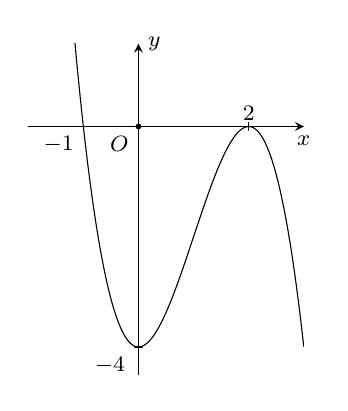
\begin{tikzpicture}[scale=0.7,line cap=round,line join=round,>=stealth, font=\footnotesize]
			\draw[->,color=black] (-2,0.) -- (3,0.) node[below] {$x$};
			\foreach \x in {2}
			\draw[shift={(\x,0)},color=black] (0pt,2pt) -- (0pt,-2pt) node[above] {$\x$};
			\draw[->,color=black] (0.,-4.5) -- (0.,1.5) node[right] {$y$};
			\foreach \y in {-4}
			\draw[shift={(0,\y)},color=black] (2pt,0pt) -- (-2pt,0pt) node[below left] {$\y$};
			\draw[color=black] (0,0) node[below left] {$O$}
			(-1,0) node[below left] {$-1$};
			\clip(-2,-4.5) rectangle (3,1.5);
			\draw[smooth,samples=100,domain=-2:3] plot(\x,{(-(\x)-1)*((\x)-2)^2});
			\fill (0cm,0cm) circle (1.5pt);
		\end{tikzpicture}
	}
	\loigiai{
		Đồ thị đã cho là đồ thị của hàm số bậc $3$ có hệ số $a<0$.
	}
\end{ex}

\begin{ex}%[2D1N5-1]%[Dự án C đề thi thử TN Môn Toán NH25-26 - Dot 4 - Huỳnh Hồ Hải]%[PhanBoiChau-KhanhHoa]%[GVPB - Phạm Văn Long]	
	\immini[thm]{Cho hàm số $f(x)=ax^3+bx^2+cx+d$ có đồ thị như hình vẽ. Hàm số đạt cực tiếu tại điểm
		\choice
		{$x=-2$}
		{$x=-1$}
		{$x=-3$}
		{\True $x=1$}}
	{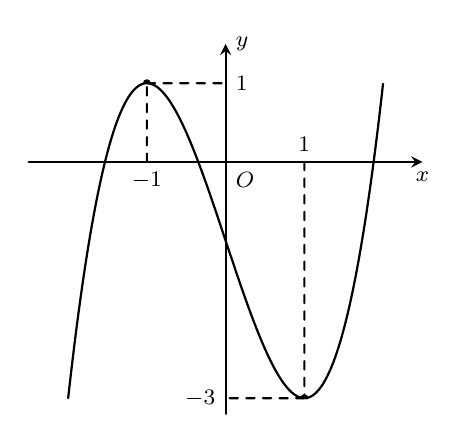
\begin{tikzpicture}[thick,line join = round, line cap = round,>=stealth,font=\footnotesize]
			\draw [->] (0,-3.2) --(0,1.5) node [right] {$y$};
			\draw [->] (-2.5,0) --(2.5,0) node [below] {$x$};
			\draw [smooth, samples=200] plot [domain=-2:2] (\x,{\x*\x*\x-3*\x-1});
			\draw (0,0) node [below right] {$O$};
			\draw [dashed](-1,0) node [below] {$-1$} --(-1,1) circle (1pt) -- (0,1) node [right] {$1$}
			(1,0) node [above] {$1$} --(1,-3) circle (1pt) -- (0,-3) node [left] {$-3$};						
	\end{tikzpicture}}
	\loigiai{
		Dựa vào đồ thị hàm số $f(x)$ đạt cực tiểu tại $x=1$.
	}
\end{ex}

\begin{ex}%[2D1V5-1]%[Dự án C đề thi thử TN Môn Toán NH25-26 - Dot 4 - Huỳnh Hồ Hải]%[PhanBoiChau-KhanhHoa]%[GVPB - Phạm Văn Long]	
	\immini[thm]{Cho hàm số $y=ax^3+bx^2+cx+d$ có đồ thị như hình vẽ dưới đây. Chọn khẳng định đúng về dấu của $a$, $d$.
		\choice
		{$a>0$, $d<0$}
		{$a<0$, $d<0$}
		{\True $ a>0$, $d>0$}
		{$a<0$, $d>0$}}
	{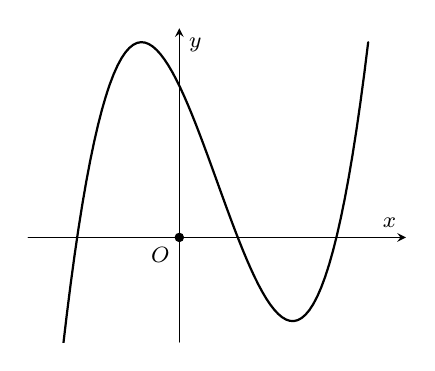
\begin{tikzpicture}[thick,line join = round, line cap = round,>=stealth,font=\footnotesize]
			\begin{axis}[scale = 0.7,
				axis lines = middle, % trục tọa độ đi qua gốc
				xtick = \empty,
				ytick = \empty,
				xlabel = {$x$},
				ylabel = {$y$},
				xmin = -2, xmax = 3,
				ymin = -1.5, ymax = 3,
				samples = 100
				]
				\addplot[domain=-2.63:2.5, thick] {(x-0.5)^3-3*(x-0.5)+0.8};
				\addplot[only marks, mark=*, mark size=1.5pt] coordinates {(0,0)}
				node[below left] {$O$};
			\end{axis}
	\end{tikzpicture}}
	\loigiai{
		Nhìn vào nhánh phải của đồ thị ta thấy đồ thị có hướng đi lên suy ra $a>0$.\\
		Nhìn vào giao điểm của đồ thị với trục tung ta thấy đồ thị cắt trục tung tại điểm có tung độ dương suy ra $d>0$.
		Vậy $a>0$, $d>0$.}
\end{ex}

\begin{ex}%[2D3H1-2]%[Dự án C - Đợt 3 - Sở Giáo Dục Sơn La]%[Nguyễn Thanh Phong - Nguyễn Tiến]
	Mỗi ngày bác Sơn đều đi bộ để rèn luyện sức khỏe. Quãng đường đi bộ mỗi ngày (đơn vị: km) của bác Sơn được thống kê ở bảng sau:
	\begin{center}
		\begin{tabular}{|c|c|c|c|c|c|}
			\hline 
			Quãng đường (km) & $[2{,}7;3{,}0)$ & $[3{,}0;3{,}3)$ & $[3{,}3;3{,}6)$ & $[3{,}6;3{,}9)$ & $[3{,}9;4{,}2)$ \\
			\hline 
			Số ngày & $3$ & $6$ & $5$ & $4$ & $2$ \\
			\hline
		\end{tabular}
	\end{center}
	Khoảng tứ phân vị của mẫu số liệu ghép nhóm trên là
	\choice
	{$0{,}975$}
	{$0{,}5$}
	{$0{,}9$}
	{\True $0{,}575$}
	\loigiai{
		Cỡ mẫu $n = 3+6+5+4+2=20$. \\
		Tứ phân vị thứ nhất thuộc nhóm $[3{,}0;3{,}3)$, do đó $Q_1 = 3{,}0 + \dfrac{\dfrac{20}{4} - 3}{6} \cdot 0{,}3 = 3{,}1$.\\
		Tứ phân vị thứ ba thuộc nhóm $[3{,}6;3{,}9)$, do đó $Q_3 = 3{,}6 + \dfrac{\dfrac{3 \cdot 20}{4} - 14}{4} \cdot 0{,}3 = 3{,}675$.\\
		Khoảng tứ phân vị của mẫu số liệu là $\Delta_Q = Q_3 - Q_1 = 3{,}675 - 3{,}1 = 0{,}575$.
	}
\end{ex}

\begin{ex}%[TT Cụm 5 - Ninh Bình-NH25-26]%[Nguyễn Chiến]%[Phản biện 1: Nguyễn Tấn Tài]%[2D3H1-3]
	Cho bảng phân bố tần số ghép lớp về độ dài của $60$ lá dương xỉ trưởng thành như sau
	\begin{center}
		\begin{tabular}{|c|c|c|c|c|}
			\hline
			Độ dài (cm) & $[10;20)$ & $[20;30)$ & $[30;40)$ & $[40;50)$ \\
			\hline
			Tần số & $7$ & $19$ & $24$ & $10$ \\
			\hline
		\end{tabular}
	\end{center}
	Tính khoảng tứ phân vị (kết quả làm tròn đến hàng phần mười) của mẫu số liệu trên.
	\choice
	{$13{,}5$}
	{$13{,}6$}
	{$13{,}8$}
	{\True $13{,}7$}
	\loigiai{
		Ta có $N=7+19+24+10=60$.
		\begin{itemize} 
			\item Ta có $\dfrac{N}{4}=\dfrac{60}{4}=15$.\\
			Nhóm chứa $Q_1$ là $[20;30)$.\\
			$Q_1=20+\dfrac{15-7}{19}\cdot 10=20+\dfrac{80}{19}=\dfrac{460}{19}$.
			\item Ta có $\dfrac{3N}{4}=\dfrac{3\cdot 60}{4}=45$.\\
			Nhóm chứa $Q_3$ là $[30;40)$.\\
			$Q_3=30+\dfrac{45-26}{24}\cdot 10=30+\dfrac{190}{24}=\dfrac{455}{12}$.
			\item Khoảng tứ phân vị là $\Delta_Q=Q_3-Q_1=\dfrac{455}{12}-\dfrac{460}{19}=\dfrac{3\,125}{228}\approx 13{,}7$.
		\end{itemize}
	}
\end{ex}

\begin{ex}%[2D3H1-3]%[Dự án đề TT Toán NH25-26-Dot 3- Bùi Lương Phúc]%[Cụm 13-Hải Phòng]%[GVPB - Viet Hoang Pham]
Mẫu số liệu ghép nhóm thống kê mức lương của một công ty (đơn vị: triệu đồng) được cho trong bảng sau
\begin{center}
\begin{tabular}{|c|c|c|c|c|c|c|}
\hline
Nhóm (triệu đồng)& $[6;8)$ & $[8;10)$ & $[10;12)$ & $[12;14)$ & $[14;16)$ &$ $\\
\hline
Tần số & $6$ & $14$ & $16$ & $12$ & $2$ &$n=50$\\
\hline
\end{tabular}
\end{center}
Tìm khoảng tứ phân vị của mẫu số liệu ghép nhóm (kết quả làm tròn đến hàng phần trăm).
\choice
{$3{,}34$}
{$3{,}16$}
{$3{,}15$}
{\True $3{,}32$}
\loigiai{
Bảng tần số tích lũy
\begin{center}
\begin{tabular}{|c|c|c|c|c|c|c|}
\hline
Nhóm (triệu đồng)& $[6;8)$ & $[8;10)$ & $[10;12)$ & $[12;14)$ & $[14;16)$ &$ $\\
\hline
Tần số & $6$ & $14$ & $16$ & $12$ & $2$ &$n=50$\\
\hline
Tần số tích lũy & $6$ & $20$ & $36$ & $48$ & $50$ &$ $\\
\hline
\end{tabular}
\end{center}
Cỡ mẫu $n=50$.\\
Vì $\dfrac{n}{4}=\dfrac{50}{4}=12{,}5$ nên $Q_1$ thuộc lớp $[8;10)$,
\[
Q_1=8+\dfrac{\dfrac{50}{4}-6}{14}\cdot2=\dfrac{125}{14}.
\]
Vì $\dfrac{3n}{4}=\dfrac{150}{4}=37{,}5$ nên $Q_3$ thuộc lớp $[12;14)$,
\[
Q_3=12+\dfrac{\dfrac{3\cdot50}{4}-36}{12}\cdot2=\dfrac{49}{4}.
\]
Suy ra $\Delta Q=Q_3-Q_1=\dfrac{49}{4}-\dfrac{125}{14}\approx3{,}32$.
}
\end{ex}

\begin{ex}%[Đề thi thử môn Toán THPT Cổ Loa, năm học 2025-2026]%[Đỗ Minh Phúc-Lê Phúc]%[2D3H1-3]
	Bảng tần số ghép nhóm sau thống kê lại cự li quả phát bóng của các vận động viên trong một giải golf (đơn vi: mét).
	\begin{center}
		\begin{tabular}{|c|c|c|c|c|c|}
			\hline Nhóm & {$[160 ; 162)$} & {$[162 ; 164)$} & {$[164 ; 166)$} & {$[166 ; 168)$} & {$[168 ; 170)$} \\
			\hline Tần số & $10$ & $25$ & $10$ & $4$ & $1$ \\
			\hline
		\end{tabular}
	\end{center}
	Khoảng tứ phân vị (đơn vị: mét) của mẫu số liệu ghép nhóm trên bằng
	\choice
	{$1{,}9$}
	{$2{,}5$}
	{\True $2{,}3$}
	{$2{,}1$}
	\loigiai{
		Ta có $n=50$.
		\begin{itemize}
			\item $Q_1 \in[162;164)$; $Q_1=162+\dfrac{\tfrac{50}{4}-10}{25} \cdot 2=162{,}2$.
			\item $Q_3 \in[164;166)$; $Q_3=164+\dfrac{\tfrac{3\cdot 50}{4}-35}{10} \cdot 2=164{,}5$.
		\end{itemize}
		Khoảng tứ phân vị của mẫu số liệu ghép nhóm trên là 
		\[\Delta Q=Q_3-Q_1=164{,}5-162{,}2=2{,}3.\]
	}
\end{ex}

\begin{ex}%[2D3H1-3]%[Đề thi thử môn Toán TRƯỜNG THPT Hàm Rồng năm học 2025-2026]%[Dương Phạm - GVPB2 Đỗ Minh Vũ]
	Cho mẫu số liệu ghép nhóm về thống kê nhiệt độ tại một địa điểm trong $30$ ngày, ta có bảng số liệu sau:
	\begin{center}
		\begin{tabular}{|l|c|c|c|c|}
			\hline
			Nhiệt độ ($^\circ C$) & $[18;21)$ & $[21;24)$ & $[24;27)$ & $[27;30)$ \\ \hline
			Số ngày & $6$ & $12$ & $9$ & $3$ \\ \hline
		\end{tabular}
	\end{center}
	Khoảng tứ phân vị của mẫu số liệu ghép nhóm là
	\choice
	{$1{,}875$}
	{$25{,}5$}
	{\True $4{,}125$}
	{$21{,}375$}
	\loigiai{
		Ta có: $n=6+12+9+3=30$.\\
		$Q_1=x_8\Rightarrow Q_1\in[21;24)\Rightarrow Q_1=21+\dfrac{\frac{30}{4}-6}{12}\cdot3=21{,}375$.\\
		$Q_3=x_{23}\Rightarrow Q_3\in[24;27)\Rightarrow Q_3=24+\dfrac{\frac{3\cdot30}{4}-18}{9}\cdot3=25{,}5$.\\
		Khoảng tứ phân vị là $\Delta Q=Q_3-Q_1=25{,}5-21{,}375=4{,}125$.
	}
\end{ex}

\begin{ex}%[2D3H2-2] %[TT-THPT Lê Thánh Tông-TPHCM-L2-NH25-26]%[Bùi Quang Phú]%[PB: Phan Anh]
	Thống kê điểm trung bình môn Toán của một số học sinh lớp $12$ được cho bởi mẫu số liệu sau
	\begin{center}
		\begin{tabular}{|l|c|c|c|c|c|c|c|}
			\hline
			Khoảng điểm & $[6{,}5;7)$ & $[7;7{,}5)$ & $[7{,}5;8)$ & $[8;8{,}5)$ & $[8{,}5;9)$ & $[9;9{,}5)$ & $[9{,}5;10]$ \\
			\hline
			Tần số & $8$ & $10$ & $16$ & $24$ & $13$ & $7$ & $4$ \\
			\hline
		\end{tabular}
	\end{center}
	Phương sai của mẫu số liệu về điểm trung bình môn Toán của một số học sinh đó là:
	\choice
	{$0{,}616$}
	{$0{,}785$}
	{$0{,}78$}
	{\True $0{,}609$}
	\loigiai{
		\begin{center}
			\begin{tabular}{|l|c|c|c|c|c|c|c|}
				\hline
				Khoảng điểm & $[6{,}5;7)$ & $[7;7{,}5)$ & $[7{,}5;8)$ & $[8;8{,}5)$ & $[8{,}5;9)$ & $[9;9{,}5)$ & $[9{,}5;10]$ \\
				\hline
				Giá trị đại diện & $6{,}75$ & $7{,}25$ & $7{,}75$ & $8{,}25$ & $8{,}75$ & $9{,}25$ & $9{,}75$ \\
				\hline
				Tần số & $8$ & $10$ & $16$ & $24$ & $13$ & $7$ & $4$ \\
				\hline
			\end{tabular}
		\end{center}
		Giá trị trung bình của mẫu số liệu ghép nhóm là
		\[\overline{x}=\dfrac{6{,}75\cdot 8+7{,}25\cdot 10+7{,}75\cdot 16+8{,}25\cdot 24+8{,}75\cdot 13+9{,}25\cdot 7+9{,}75\cdot4}{8+10+16+24+13+7+4}=\dfrac{333}{41}.\]
		Phương sai của mẫu số liệu ghép nhóm là
		\[\begin{aligned}
			S^2&=\dfrac{6{,}75^2\cdot 8+7{,}25^2\cdot 10+7{,}75^2\cdot 16+8{,}25^2\cdot 24+8{,}75^2\cdot 13+9{,}25^2\cdot 7+9{,}75^2\cdot4}{8+10+16+24+13+7+4}-\left(\dfrac{333}{41}\right)^2\\
			& \approx 0{,}609.
		\end{aligned}\]
	}
\end{ex}

\begin{ex}%[2D3H2-2]%[Dự án C đề thi thử TN Môn Toán NH25-26 - Dot 4 - Huỳnh Hồ Hải]%[PhanBoiChau-KhanhHoa]%[GVPB - Phạm Văn Long]	
	Cho hai mẫu số liệu ghép nhóm $ A$ và $ B$ có bảng tần số ghép nhóm như sau:\\
	\centerline{\begin{tabular}{|c|c|c|c|c|c|}
			\hline
			Nhóm $ A$ & $[1{,}6;1{,}8)$ & $[1{,}8;2{,}0)$ & $[2{,}0;2{,}2)$ & $[2{,}2;2{,}4)$ & $[2{,}4;2{,}6)$\\
			\hline
			Tần số & 12 & 25 & 18 & 10 & 2\\
			
			\hline
			Nhóm $ B$ & $[2{,}0;2{,}2)$ & $[2{,}2;2{,}4)$ & $[2{,}4;2{,}6)$ & $[2{,}6;2{,}8)$ & $[2{,}8;3{,}0)$\\
			\hline
			Tần số & 24 & 50 & 36 & 20 & 4\\
			\hline
	\end{tabular}}\\
	Gọi $ S_A^2$ và $ S_B^2$ lần lượt là phương sai của mẫu số liệu ghép nhóm $ A$ và $ B$. Khẳng định nào sau đây đúng?
	\choice
	{$ S_B^2=4S_A^2$}
	{$ S_A^2=S_B^2-0,16$}
	{\True $ S_A^2=S_B^2$}
	{$ S_B^2=2S_A^2$}
	\loigiai{
		Ta có
		\[\overline{x}_A=\dfrac{12\cdot 1{,}7+25\cdot 1{,}9+18\cdot 2{,}1+10\cdot 2{,}3+2\cdot 2{,}5}{12+25+18+10+2}\approx 1{,}996.\]
		Suy ra \[\begin{aligned}
			S_A^2&=\dfrac{12(1{,}7-1{,}996)^2+25(1{,}9-1{,}996)^2+18(2{,}1-1{,}996)^2+10(2{,}3-1{,}996)^2+2(2{,}5-1{,}996)^2}{12+25+18+10+2}\\ 
			&\approx 0{,}0434.\\ 
		\end{aligned}\]
		Ta có
		\[\overline{x}_B=\dfrac{24\cdot 2{,}1+50\cdot 2{,}3+36\cdot 2{,}5+20\cdot 2{,}7+4\cdot 2{,}9}{24+50+36+20+4}\approx 2{,}396.\]
		Suy ra \[\begin{aligned}
			S_B^2&=\dfrac{24(2{,}1-2{,}396)^2+50(2{,}3-2{,}396)^2+36(2{,}5-2{,}396)^2+20(2{,}7-2{,}396)^2+4(2{,}9-2{,}396)^2}{24+50+36+20+4}\\ 
			&\approx 0{,}0434.\\ 
		\end{aligned}\]\\
		Vậy $S_A^2=S_B^2$.}
\end{ex}

\begin{ex}%[2D3N1-2]%[Dự án C đề thi thử TN Môn Toán NH25-26 - Dot 4 - Thy Nguyen Vo Diem]%[Liên trường THPT cụm 09 - Đợt 2 - Hà Nội]%[GVPB - Thanh Phát]
	Thống kê điểm thi tốt nghiệp môn Toán THPT năm $2024$ của một lớp $12$ thu được kết quả như sau:
	\begin{center}
		\begin{tabular}{|c|c|c|c|c|c|c|c|}
			\hline
			Nhóm & $[3;4)$ & $[4;5)$ & $[5;6)$ & $[6;7)$ & $[7;8)$ & $[8;9)$ & $[9;10]$ \\
			\hline
			Tần số & $3$ & $4$ & $5$ & $10$ & $15$ & $10$ & $0$ \\
			\hline
		\end{tabular}
	\end{center}
	Khoảng biến thiên của mẫu số liệu thống kê trên bằng
	\choice
	{$7$}
	{\True $6$}
	{$10$}
	{$8$}
	\loigiai{
		Khoảng biến thiên của mẫu số liệu ghép nhóm là $R = 9 - 3 = 6$.
	}
\end{ex}

\begin{ex}%[2D3N1-2]%[Dự án đề TT Toán NH25-26-Dot 3- Bùi Lương Phúc]%[Cụm 13-Hải Phòng]%[GVPB - Viet Hoang Pham]
Thống kê điểm kiểm tra toán của học sinh hai lớp 12A và 12B được mẫu số liệu ghép nhóm như sau.
\begin{center}
\begin{tabular}{|c|c|c|c|c|c|}
\hline
Điểm & $[0;2)$ & $[2;4)$ & $[4;6)$ & $[6;8)$ & $[8;10)$ \\
\hline
Lớp 12A & $0$ & $1$ & $10$ & $15$ & $17$ \\
\hline
Lớp 12B & $1$ & $5$ & $17$ & $10$ & $9$ \\
\hline
\end{tabular}
\end{center}
Gọi $R_A$ và $R_B$ lần lượt là khoảng biến thiên của hai lớp 12A và 12B. Giá trị $R_A+R_B$ bằng
\choice
{$14$}
{$20$}
{$25$}
{\True $18$}
\loigiai{
Lớp 12A có $R_A=10-2=8$.\\
Lớp 12B có $R_B=10-0=10$.\\
Suy ra $R_A+R_B=18$.
}
\end{ex}

\begin{ex}%[2D3N1-2]%[Đề thi thử môn Toán TRƯỜNG THPT Hàm Rồng năm học 2025-2026]%[Dương Phạm - GVPB2 Đỗ Minh Vũ]
	Bảng sau thống kê cân nặng của 30 học sinh lớp 12A1:
	\begin{center}
		\begin{tabular}{|l|c|c|c|c|c|}
			\hline
			Cân nặng (Kg) & $[45;50)$ & $[50;55)$ & $[55;60)$ & $[60;65)$ & $[65;70)$ \\ \hline
			Số học sinh & $5$ & $10$ & $5$ & $8$ & $2$ \\ \hline
		\end{tabular}
	\end{center}
	Khoảng biến thiên của mẫu số liệu ghép nhóm trên là
	\choice
	{$70$}
	{$45$}
	{$5$}
	{\True $25$}
	\loigiai{
		Khoảng biến thiên của mẫu số liệu ghép nhóm đã cho là hiệu số giữa đầu mút phải của nhóm cuối cùng và đầu mút trái của nhóm đầu tiên $R=70-45=25$.
	}
\end{ex}

\begin{ex}%[2D3N1-2]%[Dự án C đề thi thử TN Môn Toán NH25-26 - Dot 4 - Sỹ Trường]%[THPT Nguyễn Trãi - Hà Nội]%[GVPB - Khắc Thiên]
	Tìm hiểu thời gian hoàn thành một bài tập (đơn vị: phút) của một số học sinh thu được kết quả sau:
	\begin{center}
		\begin{tabular}{|l|c|c|c|c|c|}
			\hline Thời gian (phút) &{$[0;4)$} &{$[4;8)$} &{$[8;12)$} &{$[12;16)$} &{$[16;20)$} \\
			\hline Số học sinh & $2$ & $4$ & $7$ & $4$ & $3$ \\
			\hline
		\end{tabular}
	\end{center}
	Khoảng biến thiên của mẫu số liệu ghép nhóm trên bằng bao nhiêu?
	\choice
	{$16$}
	{$4$}
	{\True $20$}
	{$15$}
	\loigiai{
		Khoảng biến thiên của mẫu số liệu ghép nhóm trên là $R=20-0=20$.
	}
\end{ex}

\begin{ex}%[2D3N1-2]%[Dự án C đề thi thử TN Môn Toán NH25-26 - Dot 4 - Huỳnh Hồ Hải]%[PhanBoiChau-KhanhHoa]%[GVPB - Phạm Văn Long]	
	Mẫu số liệu thống kê điểm trung bình cuối học kì I môn Toán cuả một số học sinh lớp $12$ được cho ở bảng sau:\\
	\centerline{\begin{tabular}{|c|c|c|c|c|c|c|c|}
			\hline
			Khoảng điểm & $[6{,}5;7)$ & $[7;7{,}5)$ & $[7{,}5;8)$ & $[8;8{,}5)$ & $[8{,}5;9)$ & $[9;9{,}5)$ & $[9{,}5;10)$\\
			\hline
			Tần số & $8$ & $10$ & $16$ & $24$ & $13$ & $7$ & $4$\\
			\hline
	\end{tabular}}\\
	Khoảng biến thiên của mẫu số liệu ghép nhóm trên là
	\choice
	{$3{,}25$}
	{\True $3{,}5$}
	{$3$}
	{$2{,}5$}
	\loigiai{
		Ta có khoảng biến thiên của mẫu số liệu là $R=10-6{,}5=3{,}5$.}	
\end{ex}

\begin{ex}%[2D3N1-3]%[Dự án C đề thi thử TN Môn Toán NH25-26 - Dot 4 - Bui Luong Phuc]%[THPT Lê Thánh Tông-TPHCM]%[GVPB - Viet Hoang Pham]
Thống kê điểm kiểm tra giữa kỳ môn Toán của học sinh lớp 11C5 được ghi lại ở bảng sau:
\begin{center}
\begin{tabular}{|l|c|c|c|c|}
\hline
Điểm & $[2;4)$ & $[4;6)$ & $[6;8)$ & $[8;10)$ \\ \hline
Số học sinh & $4$ & $8$ & $11$ & $7$ \\ \hline
\end{tabular}
\end{center}
Trung vị $Q_2$ của mẫu số liệu trên thuộc khoảng nào trong các khoảng dưới đây?
\choice
{$[2;4)$}
{$[4;6)$}
{\True $[6;8)$}
{$[8;10)$}
\loigiai{
Tổng số học sinh là $n = 4 + 8 + 11 + 7 = 30$. \\
Ta có bảng tần số tích lũy như sau
\begin{center}
\begin{tabular}{|l|c|c|c|c|}
\hline
Điểm & $[2;4)$ & $[4;6)$ & $[6;8)$ & $[8;10)$ \\ \hline
Số học sinh & $4$ & $8$ & $11$ & $7$ \\ \hline
Tần số tích lũy & $4$ & $12$ & $23$ & $30$ \\ \hline
\end{tabular}
\end{center}
Ta có $\dfrac{n}{2} = 15$ và vì $12 < 15 < 23$ nên trung vị $Q_2$ thuộc nhóm thứ ba, tức là khoảng $[6;8)$.
}
\end{ex}

\begin{ex}%[2D3N2-1]%[Dự án C đề thi thử TN Môn Toán NH25-26 - Dot 4 - Sỹ Trường]%[THPT Nguyễn Trãi - Hà Nội]%[GVPB - Khắc Thiên]
	Một mẫu số liệu ghép nhóm có độ lệch chuẩn bằng $3$ thì có phương sai bằng
	\choice
	{$s^2=6$}
	{$s^2=3$}
	{\True $s^2=9$}
	{$s^2=\sqrt{3}$}
	\loigiai{
		Phương sai của mẫu số liệu ghép nhóm có độ lệch chuẩn bằng $3$ là $s^2=3^2=9$.
	}
\end{ex}

\begin{ex}%[TT Cụm 5 - Ninh Bình-NH25-26]%[Nguyễn Chiến]%[Phản biện 1: Nguyễn Tấn Tài]%[2D4H1-2]
	Cho $F(x)$ là nguyên hàm của hàm số $f(x)=6x^5+\dfrac{1}{x^3}$ thỏa mãn $F(1)=0$. Tìm $F(x)$.
	\choice
	{$F(x)=x^6-\dfrac{1}{2x^2}+\dfrac{1}{2}$}
	{$F(x)=x^6+\dfrac{1}{2x^2}-\dfrac{3}{2}$}
	{\True $F(x)=x^6-\dfrac{1}{2x^2}-\dfrac{1}{2}$}
	{$F(x)=x^6-\dfrac{3}{x^2}+2$}
	\loigiai{
		Ta có $f(x)=6x^5+\dfrac{1}{x^3}\Rightarrow F(x)=\displaystyle\int f(x)\mathrm{\,d}x=\displaystyle\int\left(6x^5+\dfrac{1}{x^3}\right)\mathrm{\,d}x=x^6-\dfrac{1}{2x^2}+C$.\\
		Khi đó $F(1)=0\Rightarrow 1^6-\dfrac{1}{2\cdot 1^2}+C=0\Rightarrow C=-\dfrac{1}{2}$.\\
		Suy ra $F(x)=x^6-\dfrac{1}{2x^2}-\dfrac{1}{2}$.
	}
\end{ex}

\begin{ex}%[2D4H1-2]%[Dự án đề TT Toán NH25-26-Dot 3-PhucChuong]%[THPT Lê Quý Đôn - Đống Đa - Hà Nội]%[GVPB - Phan Quốc Trí]
 	Họ tất cả các nguyên hàm của hàm số $f(x) = x^3 + 2026$ là
 	\choice
 	{$\dfrac{x^4}{4} + 2026x$}
 	{\True $\dfrac{x^4}{4} + 2026x + C$}
 	{$4x^4 + 2026x + C$}
 	{$3x^2 + C$}
 	\loigiai{
 		Ta có $\displaystyle \int (x^3 + 2026)\,\mathrm{d}x = \dfrac{x^4}{4} + 2026x + C$.
 	}
 \end{ex}

\begin{ex}%[2D4H1-3]%[Dự án C đề thi thử TN Môn Toán NH25-26 - Dot 4 - Thy Nguyen Vo Diem]%[Liên trường THPT cụm 09 - Đợt 2 - Hà Nội]%[GVPB - Thanh Phát]
	Họ tất cả các nguyên hàm của hàm số $f(x) = \cos x + 6x$ là
	\choice
	{$-\sin x + 3x^2 + C$}
	{\True $\sin x + 3x^2 + C$}
	{$\sin x + 6x^2 + C$}
	{$-\sin x + C$}
	\loigiai{
		Ta có
		$$\displaystyle\int f(x) \mathrm{\,d}x =\displaystyle \int (\cos x + 6x) \mathrm{\,d}x = \sin x + 6 \cdot \dfrac{x^2}{2} + C = \sin x + 3x^2 + C.$$
	}
\end{ex}

\begin{ex}%[Đề thi thử môn Toán THPT Cổ Loa, năm học 2025-2026]%[Đỗ Minh Phúc-Lê Phúc]%[2D4H1-3]
	Họ tất cả các nguyên hàm của hàm số $f(x)=\sin x+\dfrac{1}{x}$ trên khoảng $(0;+\infty)$ là
	\choice
	{$\cos x+\ln x+C$}
	{$-\cos x-\dfrac{1}{x^2}+C$}
	{$\cos x-\dfrac{1}{x^2}+C$}
	{\True $-\cos x+\ln x+C$}
	\loigiai{
		Trên khoảng $(0;+\infty)$ ta có $\displaystyle\int f(x)\mathrm{\,d}x=\displaystyle\int \left(\sin x+\dfrac{1}{x}\right)\mathrm{\,d}x=-\cos x+\ln x+C$.
	}
\end{ex}

\begin{ex}%[2D4H1-3]%[Dự án đề TT Toán NH25-26-Dot 3-PhucChuong]%[THPT Trần Nhân Tông - Hà Nội]%[GVPB - Phan Quốc Trí]
	Họ nguyên hàm của hàm số $f(x)=\sin 2x+\cos 2x$ là
	\choice
	{$2(-\cos 2x+\sin 2x)+C$}
	{$\dfrac{1}{2}(\cos 2x-\sin 2x)+C$}
	{\True $\dfrac{1}{2}(\sin 2x-\cos 2x)+C$}
	{$2(\cos 2x-\sin 2x)+C$}
	\loigiai{Ta có $\displaystyle\int(\sin 2x + \cos 2x) \;\mathrm{d}x = \dfrac{1}{2}(-\cos 2x + \sin 2x) + C$.}
\end{ex}

\begin{ex}%[2D4H1-4]%[Dự án C đợt 3 NH25-26- Nguyễn Hữu Đức]%[SỞ GIÁO DỤC - TUYÊN QUANG]%[GVPB: Thanh Phát]
	Họ nguyên hàm của hàm số $f(x) = 2^x - x$ là  
	\choice
	{$\dfrac{2^{x+1}}{x+1} - \dfrac{x^2}{2} + C$}  
	{\True $\dfrac{2^x}{\ln 2} - \dfrac{x^2}{2} + C$}  
	{$x\cdot 2^{x-1} - \dfrac{x^2}{2} + C$}  
	{$\dfrac{2^x}{x} - \dfrac{x^2}{2} + C$}  
	\loigiai{
		Ta có $\displaystyle\int (2^x-x)\mathrm{\,d}x=\dfrac{2^x}{\ln 2}-\dfrac{x^2}{2} + C$.
	}
\end{ex}

\begin{ex}%[2D4H2-1][GV Biên Soạn: Thầy Hải Toán]%[GVPB - ThanhTa]
	Cho hàm số $f(x)$ liên tục trên $\mathbb{R}$, thỏa mãn $\displaystyle\int\limits_0^4f(x) \mathrm{\,d}x=-3$ và $\displaystyle\int\limits_4^3f(x) \mathrm{\,d}x=2$. Khi đó, $\displaystyle\int\limits_0^3f(x) \mathrm{\,d}x$ bằng
	\choice
	{\True $-5$}
	{$-1$}
	{$1$}
	{$5$}
	\loigiai{
		Ta có \allowdisplaybreaks
		\begin{eqnarray*}
			&&\displaystyle\int\limits_0^4f(x) \mathrm{\,d}x=-3\\
			&\Rightarrow& \displaystyle\int\limits_0^3 f(x) \mathrm{\,d}x + \displaystyle\int\limits_3^4(x) \mathrm{\,d}x=-3\\
			&\Leftrightarrow& \displaystyle\int\limits_0^3 f(x) \mathrm{\,d}x=-3-\displaystyle\int\limits_3^4(x) \mathrm{\,d}x\\
			&\Leftrightarrow& \displaystyle\int\limits_0^3 f(x) \mathrm{\,d}x=-3-2\\
			&\Leftrightarrow& \displaystyle\int\limits_0^3 f(x) \mathrm{\,d}x=-5.
		\end{eqnarray*}
	}
\end{ex}

\begin{ex}%[2D4H2-2]%[Dự án C đề thi thử TN Môn Toán NH25-26 - Dot 4 - Hồng Trường Sơn]%[THPT Mai Anh Tuấn - Thanh Hóa]%[GVPB - Lê Hữu Kiệt]
	Biết $\displaystyle\int\limits_1^3 \dfrac{x+2}{x}\mathrm{\,d}x=a+b\ln c$ với $a$, $b$, $c\in \mathbb{Z}$, $c<9$. Tính tổng $S=a+b+c$.
	\choice
	{$S=9$}
	{$S=8$}
	{\True $S=7$}
	{$S=6$}
	\loigiai{
		Ta có
		\allowdisplaybreaks
		\begin{eqnarray*}
			\displaystyle\int\limits_1^3 \dfrac{x+2}{x} \mathrm{\,d}x &=& \displaystyle\int\limits_1^3 \left( 1+\dfrac{2}{x} \right)\mathrm{d}x\\
			&=& \left( x+2\ln |x| \right)\Big| _1^3\\
			&=& \left( 3+2\ln 3 \right)-\left( 1+2\ln 1 \right)\\
			&=& 2+2\ln 3.
		\end{eqnarray*}
		Vậy $a=2$, $b=2$, $c=3$ suy ra $S=a+b+c=7$.
	}
\end{ex}

\begin{ex}%[2D4H3-1] %[TT-THPT Lê Thánh Tông-TPHCM-L2-NH25-26]%[Bùi Quang Phú]%[PB: Phan Anh]
	\immini[thm]{Diện tích hình phẳng được tô màu trong hình bên là
		\choice
		{$S=\displaystyle\int\limits_{1}^{3} \left(2^x-2\right)\mathrm{d}x$}
		{$S=\displaystyle\int\limits_{1}^{3} \left(2^x+2\right)\mathrm{d}x$}
		{\True $S=\displaystyle\int\limits_{1}^{3} \left(2^x-2\right)\mathrm{d}x$}
		{$S=\displaystyle\int\limits_{1}^{3} 2^x \mathrm{d}x$}}{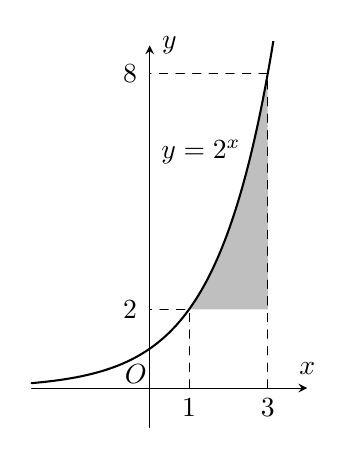
\begin{tikzpicture}[scale=.5,>=stealth,line join=round,line cap=round]
			\tikzset{label style/.style={font=\footnotesize}}
			%%Nhập giới hạn đồ thị và hàm số cần vẽ
			\def \xmin{-3}
			\def \xmax{4}
			\def \ymin{-1}
			\def \ymax{8.7}
			%%Tự động
			\draw[->] (\xmin,0)--(\xmax,0) node[shift=(90:0.25)] {$x$};
			\draw[->] (0,\ymin)--(0,\ymax) node[shift=(0:0.25)] {$y$};
			\draw (0,0) node [shift=(135:0.25)] {$O$};
			\clip(\xmin-0.1,\ymin-0.1) rectangle (\xmax+0.1,\ymax+0.1);
			%%Vẽ các điểm trên 2 hệ trục
			\fill[gray!50,draw=none] (1,2)--plot[samples=350,domain=1:3,smooth,variable=\x] (\x,{2^(\x)})--(3,2)--cycle;
			\draw[samples=350,domain=-3:3.2,smooth,variable=\x,line width=0.75pt] plot (\x,{2^(\x)});
			\draw[dashed] (1,0) |- (0,2)  (3,0) |- (0,8) ;
			\draw (1.3,6) node{$y=2^x$};
			\draw 
			(0,8) node[shift=(180:0.25)] {$8$}
			(0,2) node[shift=(180:0.25)] {$2$}
			(1,0) node[shift=(-90:0.25)] {$1$}
			(3,0) node[shift=(-90:0.25)] {$3$}
			;
	\end{tikzpicture}}
	\loigiai{
		Hình phẳng $(H)$ giới hạn bởi các đường $y=2^x$, $y=2$, các đường thẳng $x=1$ và $x=3$.\\
		Do đó $S_{(H)}=\displaystyle\int\limits_{1}^{3} \left(2^x-2\right)\mathrm{d}x$.
	}
\end{ex}

\begin{ex}%[2D4H3-3]%[Dự án C đề thi thử TN Môn Toán NH25-26 - Dot 4 - Bui Luong Phuc]%[THPT Lê Thánh Tông-TPHCM]%[GVPB - Viet Hoang Pham]
Xét hình phẳng $(H)$ giới hạn bởi đồ thị hàm số $y=x^2-4x+4$, trục tung, trục hoành và đường thẳng $x=3$. Thể tích khối tròn xoay tạo thành khi quay hình phẳng $(H)$ quanh trục $Ox$ bằng
\choice
{$33$}
{$\dfrac{33}{5}$}
{\True $\dfrac{33\pi}{5}$}
{$33\pi$}
\loigiai{
Ta có $y=x^2-4x+4=(x-2)^2\geq 0$.\\
Suy ra $V_H = \pi \displaystyle \int\limits_0^3 \left(x^2-4x+4\right)^2 \mathrm{d}x = \pi \displaystyle \int\limits_0^3 (x-2)^4 \,\mathrm{d}x = \pi \left[ \dfrac{(x-2)^5}{5} \right]\Bigg|_0^3 = \dfrac{33\pi}{5}$.
}
\end{ex}

\begin{ex}%[2D4H3-3]%[TT-THPT Lê Thánh Tông-TPHCM-L2-NH25-26]%[Bùi Quang Phú]%[PB: Phan Anh]
	Thể tích vật thể tròn xoay sinh ra khi quay hình phẳng giới hạn bởi các đường cong $y=\sqrt{\mathrm{e}^x-x}$, $y=0$, $x=1$, $x=2$ quanh trục $Ox$ là
	\choice
	{\True $\pi\left(\mathrm{e}^2-\mathrm{e}-\dfrac{3}{2}\right)$}
	{$\mathrm{e}^2-\mathrm{e}-\dfrac{5}{2}$}
	{$\pi\left(\mathrm{e}^2-\mathrm{e}-\dfrac{5}{2}\right)$}
	{$\mathrm{e}^2-\mathrm{e}-\dfrac{3}{2}$}
	\loigiai{
		Thể tích vật thể tròn xoay khi quay hình phẳng giới hạn bởi các đường cong $y=\sqrt{\mathrm{e}^x-x}$, $y=0$, $x=1$, $x=2$ xung quanh trục $Ox$ là
		\[V=\pi\displaystyle\int\limits_{1}^{2} \left(\sqrt{\mathrm{e}^x-x}\right)^2\mathrm{d}x=\pi\left.\left(\mathrm{e}^x-\dfrac{x^2}{2}\right)\right|_{1}^{2}=\pi\left(\mathrm{e}^2-\mathrm{e}-\dfrac{3}{2}\right).\]
	}
\end{ex}

\begin{ex}%[2D4H3-5]%[TT-THPT Lê Thánh Tông-TPHCM-L2-NH25-26]%[Bùi Quang Phú]%[PB: Phan Anh]
	Khối trụ có bán kính đáy $R$ và chiều cao $h$. Thể tích khối trụ được tính theo công thức
	\choice
	{$V=2\pi R^2h$}
	{$V=\dfrac{4}{3}\pi R^2h$}
	{$V=\dfrac{1}{3}\pi R^2h$}
	{\True $V=\pi R^2h$}
	\loigiai{
		\immini[thm]{Với các số thực dương $R$ và $h$, ta xét hình phẳng $(H)$ giới hạn bởi $y=R$, trục $Ox$, các đường thẳng $x=0$ và $x=h$.\\
			Quay hình phẳng $(H)$ quanh trục $Ox$ ta thu được vật thể là hình trụ.\\
			Khi đó thể tích vật thể là $V=\pi \displaystyle\int\limits_{0}^{h} R^2 \mathrm{d}x=\pi R^2h$.}{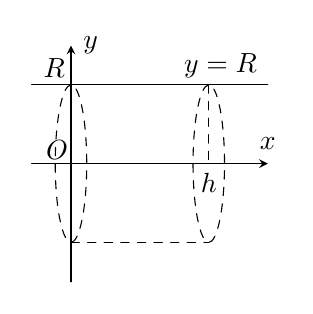
\begin{tikzpicture}[scale=.5,>=stealth,line join=round,line cap=round]
				\tikzset{label style/.style={font=\footnotesize}}
				%%Nhập giới hạn đồ thị và hàm số cần vẽ
				\def \xmin{-1}
				\def \xmax{5}
				\def \ymin{-3}
				\def \ymax{3}
				%%Tự động
				\draw[->] (\xmin,0)--(\xmax,0) node[shift=(90:0.25)] {$x$};
				\draw[->] (0,\ymin)--(0,\ymax) node[shift=(0:0.25)] {$y$};
				\draw (0,0) node [shift=(135:0.25)] {$O$};
				\clip(\xmin-0.1,\ymin-0.1) rectangle (\xmax+0.1,\ymax+0.1);
				%%Vẽ các điểm trên 2 hệ trục
				\draw (\xmin,2)--(\xmax,2)node[xshift=-0.6cm,shift=(90:0.24)] {$y=R$};
				\draw[dashed] (3.5,2)--(3.5,0)node[shift=(-90:0.25)]{$h$} (0,-2)--(3.5,-2);
				\draw[dashed] (3.5,2) arc[start angle=90,end angle=450,x radius=0.4cm,y radius =2cm] ;
				\draw[dashed] (0,2) arc[start angle=90,end angle=450,x radius=0.4cm,y radius =2cm] ;
				\draw (0,2) node[shift=(135:0.3)] {$R$};
		\end{tikzpicture}}
	}
\end{ex}

\begin{ex}%[TT Cụm 5 - Ninh Bình-NH25-26]%[Nguyễn Chiến]%[Phản biện 1: Nguyễn Tấn Tài]%[2D4N1-1]
	Biết $\displaystyle\int g(x)\mathrm{\,d}x=G(x)+C$ (với $C$ là hằng số). Khi đó khẳng định nào sau đây đúng?
	\choice
	{$g'(x)=G(x)+C$}
	{\True $G'(x)=g(x)$}
	{$G'(x)=g(x)-C$}
	{$g'(x)=G(x)$}
	\loigiai{
		$\displaystyle\int g(x)\mathrm{\,d}x=G(x)+C\Leftrightarrow G'(x)=g(x)$.
	}
\end{ex}

\begin{ex}%[2D4N1-2]%[Dự án C đề thi thử TN Môn Toán NH25-26 - Dot 4 - Hồng Trường Sơn]%[THPT Mai Anh Tuấn - Thanh Hóa]%[GVPB - Lê Hữu Kiệt]
	Họ tất cả các nguyên hàm của hàm số $f(x)=2x+6$ là
	\choice
	{$2x^2+C$}
	{$2x^2+6x+C$}
	{$x^2+C$}
	{\True $x^2+6x+C$}
	\loigiai{
		Ta có $\displaystyle\int f(x)\mathrm{\,d}x=\displaystyle\int (2x+6)\mathrm{\,d}x=x^2+6x+C$.
	}
\end{ex}

\begin{ex}%[2D4N1-3]%[Dự án C đề thi thử TN Môn Toán NH25-26 - Đợt 4 - Đỗ Minh Phúc]%[Lần 1 Liên trường Hà Nội]%[GVPB - Lê Phúc]
	Họ nguyên hàm của hàm số $f(x)=6x^2+\sin x$ là
	\choice
	{\True $2x^3-\cos x+C$}
	{$2x^3+\cos x+C$}
	{$3x^2-\cos x+C$}
	{$12x+\cos x+C$}
	\loigiai{
		Ta có $F(x)=\displaystyle\int f(x) \mathrm{\,d}x=\displaystyle\int\left(6 x^2+\sin x\right) \mathrm{\,d}x=2 x^3-\cos x+C$.
	}
\end{ex}

\begin{ex}%[2D4N1-3][GV Biên Soạn: Thầy Hải Toán]%[GVPB - ThanhTa]
	Họ nguyên hàm của hàm số $f(x)=\sin x$ là
	\choice
	{$F(x)=-\tan x+C$}
	{$F(x)=\cos x+C$}
	{\True $F(x)=-\cos x+C$}
	{$F(x)=\tan x+C$}
	\loigiai{
		$\displaystyle\int \sin{x} \mathrm{\,d}x=-\cos{x}+C$.
	}
\end{ex}

\begin{ex}%[2D4N1-3]%[Dự án C - Đợt 3 - Sở Giáo Dục Sơn La]%[Nguyễn Thanh Phong - Nguyễn Tiến]
	Họ tất cả các nguyên hàm của hàm số $y = \sin x + \cos x$ là
	\choice
	{$\displaystyle\int (\sin x + \cos x)\mathrm{\,d}x = \sin x + \cos x + C$}
	{$\displaystyle\int (\sin x + \cos x)\mathrm{\,d}x = -\sin x - \cos x + C$}
	{$\displaystyle\int (\sin x + \cos x)\mathrm{\,d}x = -\sin x + \cos x + C$}
	{\True $\displaystyle\int (\sin x + \cos x)\mathrm{\,d}x = \sin x - \cos x + C$}
	\loigiai{
		Ta có $\displaystyle\int (\sin x + \cos x)\mathrm{\,d}x = -\cos x + \sin x + C = \sin x - \cos x + C$.
	}
\end{ex}

\begin{ex}%[2D4N1-4]%[Dự án đề thi thử NH25-26]%[THPT Chuyên Phan Bội Châu - Nghệ An]%[GVPB2 Khắc Thiên]
	Họ nguyên hàm của hàm số $f(x)=5^x$ là
	\choice
	{\True $\dfrac{5^x}{\ln 5}+C$}
	{$\dfrac{5^{x+1}}{x+1}+C$}
	{$5^x+C$}
	{$5^x \cdot \ln 5+C$}
	\loigiai{
		Theo công thức nguyên hàm cơ bản, ta có $\displaystyle\int 5^x \mathrm{\,d}x = \dfrac{5^x}{\ln 5} + C$.
	}
\end{ex}

\begin{ex}%[2D4N1-4]%[Dự án C đề thi thử TN Môn Toán NH25-26 - Dot 4 - Bui Luong Phuc]%[THPT Lê Thánh Tông-TPHCM]%[GVPB - Viet Hoang Pham]
Nguyên hàm của hàm số $f(x)=4^x$ là
\choice
{$\dfrac{4^{x+1}}{x+1}+C$}
{\True $\dfrac{4^x}{2\ln 2}+C$}
{$\dfrac{4^x}{x}+C$}
{$x \cdot 4^{x-1}+C$}
\loigiai{
Ta có $\displaystyle \int f(x) \,\text{d}x = \int 4^x \,\text{d}x = \dfrac{4^x}{\ln 4} + C = \dfrac{4^x}{2\ln 2} + C$.
}
\end{ex}

\begin{ex}%[2D4N1-4]%[TT-THPT Nguyễn Trung Thiên-Hà Tĩnh-L2-NH25-26]%[Bùi Quang Phú]%[GVPB2 PhanAnh]
	Cho hàm số $f(x)=3^x+\sin x$. Một nguyên hàm của $f(x)$ trên $\mathbb{R}$ là
	\choice
	{$F(x)=3^x\ln 3 + \cos x$}
	{$F(x)=\dfrac{3^x}{\ln 3}-\sin x$}
	{\True $F(x)=\dfrac{3^x}{\ln 3}-\cos x$}
	{$F(x)=3^x+\sin x$}
	\loigiai{
	Ta có $\displaystyle\int f(x) \mathrm{\,d}x=\displaystyle\int \left(3^x+\sin x\right) \mathrm{\,d}x=\dfrac{3^x}{\ln 3}-\cos x+C$.\\
	Chọn $C=0$, được một nguyên hàm của $f(x)$ là $F(x)=\dfrac{3^x}{\ln 3}-\cos x$.
	}
\end{ex}

\begin{ex}%[2D4N2-1]%[Dự án C đề thi thử TN Môn Toán NH25-26 - Dot 4 - Thy Nguyen Vo Diem]%[Liên trường THPT cụm 09 - Đợt 2 - Hà Nội]%[GVPB - Thanh Phát]
	Cho hàm số $f(x)$ liên tục trên đoạn $[1;5]$. Biết $\displaystyle \int \limits_1^3 f(x) \mathrm{\,d}x = 4$ và $\displaystyle \int \limits_3^5 f(x) \mathrm{\,d}x = -2$. Giá trị của $I = \displaystyle \int \limits_1^5 f(x) \mathrm{\,d}x$ bằng
	\choice
	{$I = 6$}
	{\True $I = 2$}
	{$I = -2$}
	{$I = -8$}
	\loigiai{
		Ta có 
		$$I = \displaystyle \int \limits_1^5 f(x) \mathrm{\,d}x = \displaystyle \int \limits_1^3 f(x) \mathrm{\,d}x + \displaystyle \int \limits_3^5 f(x) \mathrm{\,d}x = 4 + (-2) = 2.$$
	}
\end{ex}

\begin{ex}%[2D4N2-1]%[Dự án C - Đợt 3 - Sở Giáo Dục Sơn La]%[Nguyễn Thanh Phong - Nguyễn Tiến]
	Cho hàm số $y = f(x)$ thỏa mãn $f(1) = -2$, $f(2) = 1$ và có đạo hàm liên tục trên đoạn $[1;2]$. Giá trị của tích phân $I = \displaystyle\int\limits_{1}^{2} f'(x)\mathrm{\,d}x$ là
	\choice
	{$I = -1$}
	{$I = 2$}
	{$I = -3$}
	{\True $I = 3$}
	\loigiai{
		Ta có $I = \displaystyle\int\limits_{1}^{2} f'(x)\mathrm{\,d}x = f(2) - f(1) = 1 - (-2) = 3$.
	}
\end{ex}

\begin{ex}%[Đề thi thử môn Toán THPT Cổ Loa, năm học 2025-2026]%[Đỗ Minh Phúc]%[2D4N2-1]%[PB1: Lê Phúc]
	Nếu $\displaystyle\int \limits_1^2 f(x) \mathrm{\,d}x=3$ và $ \displaystyle\int \limits_1^5 f(x) \mathrm{\,d}x=-2$ thì $ \displaystyle\int \limits_2^5 f(x) \mathrm{\,d}x$ bằng
	\choice
	{$1$}
	{$6$}
	{$-3$}
	{\True $-5$}
	\loigiai{
		Ta có $\displaystyle\int \limits_2^5 f(x) \mathrm{\,d}x=\displaystyle\int \limits_1^5 f(x) \mathrm{\,d}x-\displaystyle\int \limits_1^2 f(x) \mathrm{\,d}x=-2-3=-5$.
	}
\end{ex}

\begin{ex}%[2D4N2-1]%[TT-THPT Nguyễn Trung Thiên-Hà Tĩnh-L2-NH25-26]%[Bùi Quang Phú]%[GVPB2 PhanAnh]
Biết $\displaystyle\int\limits_{-1}^{1} f(x) \mathrm{\,d}x=3$, khi đó $\displaystyle\int\limits_{-1}^{1} \left[2f(x)+1\right]\mathrm{\,d}x$ bằng
	\choice
	{\True $8$}
	{$10$}
	{$7$}
	{$6$}
	\loigiai{
	Ta có $\displaystyle\int\limits_{-1}^{1} \left[2f(x)+1\right]\mathrm{\,d}x=2\displaystyle\int\limits_{-1}^{1} f(x) \mathrm{\,d}x+\displaystyle\int\limits_{-1}^{1} 1 \mathrm{\,d}x=2\cdot3+2=8$.
	}
\end{ex}

\begin{ex}%[2D4N3-1]%[Dự án đề TT Toán NH25-26-Dot 3- Văn Minh Thoại]%[SGD Tuyên Quang-L1]%[GVPB: Thanh Phát]
	Trong mặt phẳng với hệ tọa độ $Oxy$, diện tích $S$ của hình phẳng giới hạn bởi đồ thị hàm số $y=x^2-2x$, trục hoành và hai đường thẳng $x=-1$, $x=3$ được xác định bằng công thức
	\choice
	{$S=\pi\displaystyle\int\limits_{-1}^{3}\left|x^2-2x\right|\mathrm{\,d}x$}
	{$S=\pi\displaystyle\int\limits_{-1}^{3}\left(x^2-2x\right)^2\mathrm{\,d}x$}
	{\True $S=\displaystyle\int\limits_{-1}^{3}\left|x^2-2x\right|\mathrm{\,d}x$}
	{$S=\left|\displaystyle\int\limits_{-1}^{3}(x^2-2x)\mathrm{\,d}x\right|$}
	\loigiai{
		Diện tích hình phẳng giới hạn bởi đồ thị hàm số $y=x^2-2x$, trục hoành và hai đường thẳng $x=-1$, $x=3$ là $S=\displaystyle\int\limits_{-1}^{3}\left|x^2-2x\right|\mathrm{\,d}x$.
	}
\end{ex}

\begin{ex}%[2D4N3-1]%[Dự án đề TT Toán NH25-26-Dot 3-PhucChuong]%[THPT Trần Nhân Tông - Hà Nội]%[GVPB - Phan Quốc Trí]
	Trong mặt phẳng $Oxy$, diện tích $S$ của hình phẳng giới hạn bởi đồ thị hàm số $y=3x-1$, trục hoành và hai đường $x=1$, $x=3$ được xác định bằng công thức nào sau đây?
	\choice
	{$S=\displaystyle\int\limits_{1}^{3} (3x-1)^2 \,\mathrm{d}x$}
	{$S=\pi \displaystyle\int\limits_{1}^{3} \left| 3x-1 \right| \,\mathrm{d}x$}
	{\True $S=\displaystyle\int\limits_{1}^{3}(3x-1) \,\mathrm{d}x$}
	{$S=\pi \displaystyle\int\limits_{1}^{3} (3x-1 )^2 \,\mathrm{d}x$}
	\loigiai{Diện tích hình phẳng giới hạn bởi đồ thị hàm số $y=3x-1$, trục hoành và hai đường $x=1$, $x=3$ được tính bằng $S = \displaystyle\int\limits_{1}^{3}(3x-1) \,\mathrm{d}x$.}
\end{ex}

\begin{ex}%[2H2H1-1]%[Dự án C đề thi thử TN Môn Toán NH25-26 - Dot 4 - Huỳnh Hồ Hải]%[PhanBoiChau-KhanhHoa]%[GVPB - Phạm Văn Long]	
	\immini[thm]{Cho hình lập phương $ABCD.A'B'C'D'$. Gọi $O$ là tâm của hình lập phương. Khẳng định nào sau đây là đúng?
		\choice
		{\True $\overrightarrow{AO}=\dfrac{1}{2}(\overrightarrow{AB}+\overrightarrow{AD}+\overrightarrow{AA'})$}
		{$\overrightarrow{AO}=\dfrac{1}{3}(\overrightarrow{AB}+\overrightarrow{AD}+\overrightarrow{AA'})$}
		{$\overrightarrow{AO}=\dfrac{2}{3}(\overrightarrow{AB}+\overrightarrow{AD}+\overrightarrow{AA'})$}
		{$\overrightarrow{AO}=\dfrac{1}{4}(\overrightarrow{AB}+\overrightarrow{AD}+\overrightarrow{AA'})$}}
	{\begin{tikzpicture}[thick,line join = round, line cap = round,>=stealth,font=\footnotesize]
			\coordinate (A) at (0,0);
			\coordinate (B) at (-1,-1.5);
			\coordinate (D) at (3,0);
			\coordinate (A') at (0,2.5);
			\coordinate (C) at ($(B)+(D)$);
			\coordinate (B') at ($(B)+(A')$);
			\coordinate (C') at ($(A')+(C)$);
			\coordinate (D') at ($(A')+(D)$);
			\draw (A') -- (B') -- (C') -- (D') --cycle;
			\draw (B) -- (B')
			(C) -- (C')
			(D) -- (D');
			\draw [dashed] (A) --(A')
			(A) -- (B)
			(A) -- (D);
			\draw (B) -- (C) -- (D);
			\foreach \i in {A,B,C,D,A',B',C',D'}{
				\fill (\i) circle (1.5pt) node [above left] {$\i$};}
	\end{tikzpicture}}	
	\loigiai{
		\begin{tikzpicture}[thick,line join = round, line cap = round,>=stealth,font=\footnotesize]
			\coordinate (A) at (0,0);
			\coordinate (B) at (-1,-1.5);
			\coordinate (D) at (3,0);
			\coordinate (A') at (0,2.5);
			\coordinate (C) at ($(B)+(D)$);
			\coordinate (B') at ($(B)+(A')$);
			\coordinate (C') at ($(A')+(C)$);
			\coordinate (D') at ($(A')+(D)$);
			\coordinate (O) at ($(A)!0.5!(C')$);
			\draw (A') -- (B') -- (C') -- (D') --cycle;
			\draw (B) -- (B')
			(C) -- (C')
			(D) -- (D');
			\draw [dashed] (A) --(A')
			(A) -- (B)
			(A) -- (D)
			(A) --(C')
			(A') -- (C);
			\draw (B) -- (C) -- (D);
			\foreach \i in {A,B,C,D,A',B',C',D'}{
				\fill (\i) circle (1.5pt) node [above left] {$\i$};}
			\fill (O) circle (1.5pt) node [below] {$O$};
		\end{tikzpicture}\\
		Ta có $\overrightarrow{AO}=\dfrac{1}{2}\overrightarrow{A{C}'}=\dfrac{1}{2}(\overrightarrow{AB}+\overrightarrow{AD}+\overrightarrow{A{A}'})$.}
	
\end{ex}

\begin{ex}%[TT Cụm 5 - Ninh Bình-NH25-26]%[Nguyễn Chiến]%[Phản biện 1: Nguyễn Tấn Tài]%[2H2H1-2]
	\immini[thm]{
		Cho hình hộp $ABCD.A_1B_1C_1D_1$. Khẳng định nào dưới đây \textbf{sai}?
		\choice
		{$\overrightarrow{AB}+\overrightarrow{AD}+\overrightarrow{AA_1}=\overrightarrow{AC_1}$}
		{\True $\overrightarrow{AB}+\overrightarrow{DD_1}=\overrightarrow{AD_1}$}
		{$\overrightarrow{AB}+\overrightarrow{CC_1}=\overrightarrow{AB_1}$}
		{$\overrightarrow{AD}+\overrightarrow{BB_1}=\overrightarrow{AD_1}$}
	}{
		\begin{tikzpicture}[line join = round, line cap=round,>=stealth,font=\footnotesize,scale=.7]
			\def\a{4}
			\def\b{2}
			\def\h{4}
			\def\g{30}
			\path
			(0,0) coordinate (B)
			(0:\a) coordinate (C)
			(\g:\b) coordinate (A)
			($(A)+(C)-(B)$) coordinate (D)
			;
			\foreach \i in {A,B,C,D} \path (\i)--++(70:\h) coordinate (\i1);
			\draw (A1)--(D1)--(D)--(C)--(B)--(B1)--(A1) (D1)--(C1)--(B1) (C)--(C1);
			\draw[dashed] (A1)--(A)--(D) (A)--(B);
			\foreach \x/\g in {A/135,B/-135,C/-45,D/-45,A1/135,B1/135,C1/-45,D1/45}\fill (\x) circle (1pt) + (\g:0.3) node {$\x$};
		\end{tikzpicture}
	}
	\loigiai{
		Ta có $\overrightarrow{AB}+\overrightarrow{DD_1}=\overrightarrow{AB}+\overrightarrow{BB_1}=\overrightarrow{AB_1}$.
	}
\end{ex}

\begin{ex}%[2H2H1-2]%[Dự án đề TT Toán NH25-26-Dot 3- Bùi Lương Phúc]%[Cụm 13-Hải Phòng]%[GVPB - Viet Hoang Pham]
Cho hình lập phương $ABCD.A'B'C'D'$ có cạnh bằng $a$. Độ dài của vectơ ${\overrightarrow{u}=\overrightarrow{A'C'}-\overrightarrow{A'A}}$ bằng
\choice
{$a\sqrt{6}$}
{\True $a\sqrt{3}$}
{$a\sqrt{2}$}
{$\dfrac{a\sqrt{3}}{2}$}
\loigiai{
\begin{center}
\begin{tikzpicture}[line join=round,line cap=round,scale=1,font=\footnotesize,>=stealth]
	\def\c{3}
	\coordinate (A') at (0,0);
	\coordinate (B') at (3,0);
	\coordinate (D') at (1,0.8);
	\coordinate (C') at ($(B')+(D')-(A')$);
	\coordinate (A) at ($(A')+(0,\c)$);
	\coordinate (B) at ($(B')+(0,\c)$);
	\coordinate (C) at ($(C')+(0,\c)$);
	\coordinate (D) at ($(D')+(0,\c)$);
	\draw (A')--(B')--(C')--(C)--(B)--(B') (B)--(A)--(D)--(C) (A')--(A) ;
	\draw[dashed] (A')--(D')--(D) (C')--(D') (A)--(C');
	\foreach \p/\g in {A'/-135,B'/-45,C'/0,D'/150,A/180,B/-30,C/45,D/135}\node at ($(\p)+(\g:0.3)$){$\p$};
\end{tikzpicture}
\end{center}
Vì $AC'$ là đường chéo của hình lập phương cạnh $a$ nên $AC'=a\sqrt{3}$.\\
Ta có \[
\left|\overrightarrow{u}\right|=\left|\overrightarrow{A'C'}-\overrightarrow{A'A}\right|=\left|\overrightarrow{AC'}\right|=AC'=a\sqrt{3}.\]
}
\end{ex}

\begin{ex}%[2H2H1-2]%[Dự án đề thi thử NH25-26]%[THPT Chuyên Phan Bội Châu - Nghệ An]%[GVPB2 Khắc Thiên]
	\immini[thm]{Cho hình chóp $S.ABCD$ có đáy $ABCD$ là hình bình hành. Tìm khẳng định đúng.
		\choice
		{$\overrightarrow{SA} - \overrightarrow{SB} = \overrightarrow{SC} - \overrightarrow{SD}$}
		{\True $\overrightarrow{SA} = \overrightarrow{SB} + \overrightarrow{CD}$}
		{$\overrightarrow{AC} = \overrightarrow{AB} + \overrightarrow{BD}$}
		{$\overrightarrow{SA} = \overrightarrow{SB} + \overrightarrow{DC}$}}{	\begin{tikzpicture}
			\tikzset{declare function={a=3; b=2; h=2.5;}}
			\path (0,0) coordinate (A)
			(a,0) coordinate (D)
			(-135:b) coordinate (B)
			($(B)+(D)$) coordinate (C)
			({0.15*a},h) coordinate (S);
			\draw[dashed] (B)--(A)--(D)
			(A)--(S);
			\draw (S)--(B)--(C)--(D)--cycle (S)--(C);
			\foreach \t/\g in {A/180,B/180,C/0,D/0,S/90}{
				\fill (\t) circle (1pt) node[shift={(\g:7pt)},font=\scriptsize]{$\t$};
			}
	\end{tikzpicture}}
	\loigiai{
		Vì tứ giác $ABCD$ là hình bình hành nên $\overrightarrow{AB} = \overrightarrow{DC} \Rightarrow -\overrightarrow{AB} = -\overrightarrow{DC} \Rightarrow \overrightarrow{BA} = \overrightarrow{CD}$.\\
		Xét khẳng định $\overrightarrow{SA} - \overrightarrow{SB} = \overrightarrow{BA}$.\\ Do đó $\overrightarrow{SA} - \overrightarrow{SB} = \overrightarrow{CD} \Leftrightarrow \overrightarrow{SA} = \overrightarrow{SB} + \overrightarrow{CD}$.
	}
\end{ex}

\begin{ex}%[2H2H1-2] %[TT-THPT Lê Thánh Tông-TPHCM-L2-NH25-26]%[Bùi Quang Phú]%[PB: Phan Anh]
	Cho tứ diện $ABCD$. Gọi $M$, $P$ là trung điểm của $AB$ và $CD$. Đặt $\overrightarrow{BA}=\overrightarrow{b}$, $\overrightarrow{AC}=\overrightarrow{c}$,  $\overrightarrow{AD}=\overrightarrow{d}$. Khẳng định nào sau đây đúng?
	\choice
	{\True $ \overrightarrow{MP}=\dfrac{1}{2}\left(\overrightarrow{c}+\overrightarrow{d}+\overrightarrow{b}\right)$}
	{$ \overrightarrow{MP}=\dfrac{1}{2}\left(\overrightarrow{d}+\overrightarrow{b}-\overrightarrow{c}\right)$}
	{$ \overrightarrow{MP}=\dfrac{1}{2}\left(-\overrightarrow{d}+\overrightarrow{b}+\overrightarrow{c}\right)$}
	{$ \overrightarrow{MP}=\dfrac{1}{2}\left(\overrightarrow{c}+\overrightarrow{d}-\overrightarrow{b}\right)$}
	\loigiai{
		\immini[thm]{
			Vì $M$ là trung điểm của $AB$ nên $\overrightarrow{MA}=\dfrac{1}{2}\overrightarrow{BA}$.\\
			Vì $P$ là trung điểm của $CD$ nên $\overrightarrow{AP}=\dfrac{1}{2}\left(\overrightarrow{AC}+\overrightarrow{AD}\right)$.\\
			Áp dụng qui tắc ba điểm ta có \[\overrightarrow{MP}=\overrightarrow{MA}+\overrightarrow{AP}=\dfrac{1}{2}\overrightarrow{BA}+\dfrac{1}{2}\left(\overrightarrow{AC}+\overrightarrow{AD}\right).\]
			Do đó $\overrightarrow{MP}=\dfrac{1}{2}\left(\overrightarrow{BA}+\overrightarrow{AC}+\overrightarrow{AD}\right)=\dfrac{1}{2}\left(\overrightarrow{c}+\overrightarrow{d}+\overrightarrow{b}\right)$.}{\begin{tikzpicture}[scale=0.7,font={\footnotesize},>=stealth]	
				\path
				(0,0) coordinate (B)
				(1.9,-1.6) coordinate (C)
				(4.5,0) coordinate (D)
				(1,3) coordinate (A)
				($(A)!1/2!(B)$) coordinate (M)
				($(C)!1/2!(D)$) coordinate (P)
				;
				
				\draw[dashed] (B)--(D) (M)--(P) ;
				\draw (B)--(C)--(D) (C)--(A)--(B) (P)--(A)--(D) ;
				% vẽ điểm
				\foreach \x/\g in {A/90,B/180,C/-90,D/0,P/-70,M/150}
				\draw[fill=black] (\x) circle (1pt)+(\g:.35)
				node{$\x$};			
		\end{tikzpicture}}
	}
\end{ex}

\begin{ex}%[2H2H1-2]%[Dự án đề TT Toán NH25-26-Dot 3-PhucChuong]%[THPT Trần Nhân Tông - Hà Nội]%[GVPB - Phan Quốc Trí]
	Cho hình hộp $ABCD.A'B'C'D'$. $O$ là tâm của đáy $ABCD$. Đẳng thức nào sau đây là \textbf{sai}?
	\choice
	{$\overrightarrow{AB}+\overrightarrow{BC'}+\overrightarrow{CD}+\overrightarrow{D'A}=\overrightarrow{0}$}
	{$\overrightarrow{AB}+\overrightarrow{BC}+\overrightarrow{CC'}=\overrightarrow{AD'}+\overrightarrow{D'O}+\overrightarrow{OC'}$}
	{$\overrightarrow{AC'}=\overrightarrow{AB}+\overrightarrow{AD}+\overrightarrow{AA'}$}
	{\True $\overrightarrow{AB}+\overrightarrow{AA'}=\overrightarrow{AD}+\overrightarrow{DD'}$}
	\loigiai{
		\immini[thm]{Ta có $\overrightarrow{AB}+\overrightarrow{AA'}=\overrightarrow{AB'}\ne\overrightarrow{AD'}=\overrightarrow{AD}+\overrightarrow{DD'}$.}{\begin{tikzpicture}[scale=.6, font=\footnotesize, line join=round, line cap=round, >=stealth]
				\path (0,0) coordinate (A)++(-2,-2) coordinate (B)++(6,0) coordinate (C)++(2,2) coordinate (D)
				\foreach \x in {A,B,C,D}{
					(\x)++(1,5) coordinate (\x')
				}
				;
				\draw[dashed] (A)--(B) (A)--(D) (A)--(A');
				\draw (A')--(B')--(C')--(D')--cycle
				(B)--(B')
				(C)--(C')
				(D)--(D')
				(B)--(C)--(D);
				\draw[->, dashed] (A)--(B');
				\draw[->, dashed] (A)--(D');
				\foreach \x/\y in {A/180,B/-135,C/-45,D/0,A'/135,B'/180,C'/-45,D'/0}{\fill (\x)node[shift={(\y:3mm)}]{$\x$} circle (1pt);}
		\end{tikzpicture}}
	}
\end{ex}

\begin{ex}%[2H2H1-3]%[Dự án C đợt 3 NH25-26- Nguyễn Hữu Đức]%[SỞ GIÁO DỤC - TUYÊN QUANG]%[GVPB: Thanh Phát]
	Cho hai vectơ $\overrightarrow{a}$ và $\overrightarrow{b}$ cùng hướng và khác vectơ $\vec{0}$. Phát biểu nào sau đây là đúng?  
	\choice
	{$\overrightarrow{a}\cdot\overrightarrow{b} = -1$}  
	{$\overrightarrow{a}\cdot\overrightarrow{b} = 0$}  
	{\True $\overrightarrow{a}\cdot\overrightarrow{b} = \left|\overrightarrow{a}\right|\cdot\left|\overrightarrow{b}\right|$}  
	{$\overrightarrow{a}\cdot\overrightarrow{b} = -\left|\overrightarrow{a}\right|\cdot\left|\overrightarrow{b}\right|$}  
	\loigiai{
		Vì $\overrightarrow{a}$ và $\overrightarrow{b}$ cùng hướng nên góc giữa chúng bằng $0^\circ$.\\  
		Ta có $\overrightarrow{a}\cdot\overrightarrow{b} =\left|\overrightarrow{a}\right|\cdot\left|\overrightarrow{b}\right| \cdot \cos 0^\circ = \left|\overrightarrow{a}\right|\cdot\left|\overrightarrow{b}\right|$.
	}
\end{ex}

\begin{ex}%[2H2H1-3]%[Dự án đề TT Toán NH25-26-Dot 3-PhucChuong]%[THPT Lê Quý Đôn - Đống Đa - Hà Nội]%[GVPB - Phan Quốc Trí]
 	Trong không gian, cho hai vectơ $\overrightarrow{u}$, $\overrightarrow{v}$ biết $\left|\overrightarrow{u}\right|=3$, $\left|\overrightarrow{v}\right|=5$ và góc giữa hai vectơ bằng $120^\circ$. Độ dài vectơ $\overrightarrow{u} + \overrightarrow{v}$ bằng
 	\choice
 	{$\left|\overrightarrow{u} + \overrightarrow{v}\right| = 7$}
 	{\True $\left|\overrightarrow{u} + \overrightarrow{v}\right| = \sqrt{19}$}
 	{$\left|\overrightarrow{u} + \overrightarrow{v}\right| = 19$}
 	{$\left|\overrightarrow{u} + \overrightarrow{v}\right| = 49$}
 	\loigiai{
 		Ta có 
 		\begin{eqnarray*}
 			&\left|\overrightarrow{u} + \overrightarrow{v}\right|^2 &= \overrightarrow{u}^2 + 2\cdot\overrightarrow{u}\cdot\overrightarrow{v} + \overrightarrow{v}^2\\
 			&&= \left|\overrightarrow{u}\right|^2 + 2\left|\overrightarrow{u}\right| \cdot \left|\overrightarrow{v}\right| \cdot \cos(\overrightarrow{u}, \overrightarrow{v}) + \left|\overrightarrow{v}\right|^2\\
 			&&= 3^2 + 2 \cdot 3 \cdot 5 \cdot \cos 120^\circ + 5^2 = 19.
 		\end{eqnarray*}
 		Vậy $\left|\overrightarrow{u} + \overrightarrow{v}\right| = \sqrt{19}$.
 	}
 \end{ex}

\begin{ex}%[2H2H2-2]%[Dự án C đề thi thử TN Môn Toán NH25-26 - Dot 4 - Thy Nguyen Vo Diem]%[Liên trường THPT cụm 09 - Đợt 2 - Hà Nội]%[GVPB - Thanh Phát]
	Trong không gian với hệ tọa độ $Oxyz$, cho hình bình hành $ABCD$ với $A(1;2;-1)$, $B(2;-1;3)$, $C(-3;5;1)$. Tọa độ điểm $D$ là
	\choice
	{\True $D(-4;8;-3)$}
	{$D(-2;2;5)$}
	{$D(0;2;5)$}
	{$D(-4;8;3)$}
	\loigiai{
		Gọi tọa độ điểm $D$ là $(x_D; y_D; z_D)$.
		Ta có
		\begin{itemize}
			\item $\overrightarrow{AD} = (x_D - 1; y_D - 2; z_D + 1)$;
			\item $\overrightarrow{BC} = (-5; 6; -2)$.
		\end{itemize}
		Vì tứ giác $ABCD$ là hình bình hành nên $\overrightarrow{AD} =\overrightarrow{BC}$. Do đó
		$$\heva{
			& x_D - 1 = -5 \\
			& y_D - 2 = 6 \\
			& z_D + 1 = -2
		}
		\Leftrightarrow
		\heva{
			& x_D = -4 \\
			& y_D = 8 \\
			& z_D = -3.
		}$$
		Vậy tọa độ điểm $D$ là $D(-4;8;-3)$.
	}
\end{ex}

\begin{ex}%[2H2H2-2]%[TT-THPT Nguyễn Trung Thiên-Hà Tĩnh-L2-NH25-26]%[Bùi Quang Phú]%[GVPB2 PhanAnh]
Trong không gian $Oxyz$, cho $A(2;-2;1), B(0;1;2)$. Tọa độ điểm $M$ thuộc mặt phẳng $(Oxy)$ sao cho ba điểm $A$, $B$, $M$ thẳng hàng là
	\choice
	{\True $M(4;-5;0)$}
	{$M(2;-3;0)$}
	{$M(4;5;0)$}
	{$M(0;0;1)$}
	\loigiai{
	Gọi $M(x;y;0)$ là điểm thuộc $(Oxy)$.\\
	Ta có $\overrightarrow{AM}=(x-2;y+2;-1)$ và $\overrightarrow{AB}=(-2;3;1)$.\\
	Vì $A$, $M$, $B$ thẳng hàng nên $\overrightarrow{AM}$ cùng phương $\overrightarrow{AB}$.\\
	Khi đó $\dfrac{x-2}{-2}=\dfrac{y+2}{3}=\dfrac{-1}{1} \Rightarrow \heva{& \dfrac{x-2}{-2}=-1  \\& \dfrac{y+2}{3}=-1 \\} \Rightarrow \heva{& x=4 \\& y=-5.\\}$\\
	Vậy $M(4;-5;0)$.
	}
\end{ex}

\begin{ex}%[2H2H2-3]%[Dự án C đề thi thử TN Môn Toán NH25-26 - Đợt 4 - Đỗ Minh Phúc]%[Lần 1 Liên trường Hà Nội]%[GVPB - Lê Phúc]
	Trong không gian $Oxyz$, cho hai vectơ $\overrightarrow{u}=(1;-1;2)$, $\overrightarrow{v}=(2;-1;-3)$. Tính độ dài của vectơ $3\overrightarrow{u}+\overrightarrow{v}$.
	\choice
	{$\sqrt{14}$}
	{$\sqrt{114}$}
	{\True $5\sqrt{2}$}
	{$3\sqrt{5}$}
	\loigiai{
		Ta có $\overrightarrow{u}=(1;-1;2) \Rightarrow 3 \overrightarrow{u}=(3;-3;6) \Rightarrow 3 \overrightarrow{u}+\overrightarrow{v}=(5;-4;3)$.\\
		Vậy $\left|3 \overrightarrow{u}+\overrightarrow{v}\right|=\sqrt{25+16+9}=5\sqrt{2}$.
	}
\end{ex}

\begin{ex}%[Đề thi thử môn Toán THPT Cổ Loa, năm học 2025-2026]%[Đỗ Minh Phúc-Lê Phúc]%[2H2H2-3]
	Trong không gian $Oxyz$, cho hai vectơ $\overrightarrow{a}=(1;2;-1)$ và $\overrightarrow{b}=(3;4;3)$. Tọa độ của vectơ $\overrightarrow{u}=\overrightarrow{a}+\overrightarrow{b}$ là
	\choice
	{\True $(4;6;2)$}
	{$(-4;-6;-2)$}
	{$(2;2;4)$}
	{$(-2;-2;-4)$}
	\loigiai{
		Vì $\overrightarrow{a}=(1;2;-1)$ và $\overrightarrow{b}=(3;4;3)$ nên $\overrightarrow{u}=\overrightarrow{a}+\overrightarrow{b}=(1+3;2+4;-1+3)=(4;6;2)$.
	}
\end{ex}

\begin{ex}%[2H2H2-3]%[Dự án C đề thi thử TN Môn Toán NH25-26 - Dot 4 - Sỹ Trường]%[THPT Nguyễn Trãi - Hà Nội]%[GVPB - Khắc Thiên]
	Trong không gian với hệ tọa độ $Oxyz$, cho $\overrightarrow{a}=(2;3;3)$, $\overrightarrow{b}=(0;-2;-1)$, $\overrightarrow{c}=(1;-2;1)$. Khi đó tọa độ của vectơ $\overrightarrow{u}=2\overrightarrow{a}+\overrightarrow{b}-\overrightarrow{c}$ là
	\choice
	{$(1;2;3)$}
	{\True $(3;6;4)$}
	{$(1;3;3)$}
	{$(3;-1;5)$}
	\loigiai{
		Ta có $\overrightarrow{u}=2\overrightarrow{a}+\overrightarrow{b}-\overrightarrow{c}=(4+0-1; 6-2+2; 6-1-1)=(3;6;4)$.
	}
\end{ex}

\begin{ex}%[2H2N1-1]%[TT-THPT Nguyễn Trung Thiên-Hà Tĩnh-L2-NH25-26]%[Bùi Quang Phú]%[GVPB2 PhanAnh]
\immini[thm]{Cho hình hộp chữ nhật $ABCD.A'B'C'D'$. Khẳng định nào đúng?
	\choice
	{\True $\overrightarrow{AD}$ cùng hướng với $\overrightarrow{B'C'}$}
	{$\overrightarrow{AC'}$ cùng hướng với $\overrightarrow{A'C'}$}
	{$\overrightarrow{CD}$ cùng hướng với $\overrightarrow{D'C'}$}
	{$\overrightarrow{AC'} = \overrightarrow{BD'}$}}{\begin{tikzpicture}[scale=0.8,font={\footnotesize},>=stealth]	
		\path
		(0,0) coordinate (A)
		(4,0) coordinate (B)
		(1.8,1.6) coordinate (D)
		($(B)+(D)-(A)$) coordinate (C)
		($(A)+(0,2.5)$) coordinate (A')
		($(B)+(0,2.5)$) coordinate (B')
		($(C)+(0,2.5)$) coordinate (C')
		($(D)+(0,2.5)$) coordinate (D')
		;
		
		\draw[dashed] (A)--(D)--(C) (D)--(D');
		\draw (A)--(B)--(C)  (A)--(A') (B)--(B') (C)--(C') (A')--(B')--(C')--(D')--(A') ;
		% vẽ điểm
		\foreach \x/\g in {A/-90,B/-90,C/0,D/160,A'/180,B'/-30,C'/90,D'/90}
		\draw[fill=black] (\x) circle (1pt)+(\g:.27)
		node{$\x$};	
		
		\end{tikzpicture}}
	\loigiai{
	Ta có $\heva{& AD \parallel BC \\& BC \parallel B'C' \\} \Rightarrow AD \parallel B'C'$.\\
	Do đó $\overrightarrow{AD}$ và $\overrightarrow{B'C'}$ cùng hướng.
	}
\end{ex}

\begin{ex}%[2H2N1-1]%[Dự án C đề thi thử TN Môn Toán NH25-26 - Dot 4 - Huỳnh Hồ Hải]%[PhanBoiChau-KhanhHoa]%[GVPB - Phạm Văn Long]		
	Cho hình chóp $S.ABC$. Mệnh đề nào sau đây đúng?
	\choice
	{$\overrightarrow{SA}-\overrightarrow{SB}=\overrightarrow{AB}$}
	{$\overrightarrow{SA}-\overrightarrow{SB}=\overrightarrow{SC}$}
	{$\overrightarrow{SA}-\overrightarrow{SB}=\overrightarrow{CS}$}
	{\True $\overrightarrow{SA}-\overrightarrow{SB}=\overrightarrow{BA}$}
	\loigiai{
		Theo quy tắc trừ vectơ ta có $\overrightarrow{SA}-\overrightarrow{SB}=\overrightarrow{BA}$.
	}
\end{ex}

\begin{ex}%[2H2N1-2]%[Dự án C đề thi thử TN Môn Toán NH25-26 - Đợt 4 - Đỗ Minh Phúc]%[Lần 1 Liên trường Hà Nội]%[GVPB - Lê Phúc]
	\immini[thm]{Cho hình lăng trụ $ABC.A'B'C'$ (xem hình vẽ bên). Phát biểu nào sau đây đúng?
		\choice
		{$\overrightarrow{BA}+\overrightarrow{A'C'}=\overrightarrow{A'A}$}
		{\True $\overrightarrow{BA}+\overrightarrow{A'C'}=\overrightarrow{BC}$}
		{$\overrightarrow{BA}+\overrightarrow{A'C'}=\overrightarrow{C'B'}$}
		{$\overrightarrow{B A}+\overrightarrow{A'C'}=\overrightarrow{BC'}$}}{\begin{tikzpicture}[scale=0.8, font=\footnotesize, line join=round, line cap=round, >=stealth]
			\coordinate (A) at (0,0); 
			\coordinate (B) at (2,-1);
			\coordinate (C) at (4,0);
			\coordinate (A') at ($(A)+(70:4)$);
			\coordinate (B') at ($(A')-(A)+(B)$);
			\coordinate (C') at ($(A')-(A)+(C)$);
			\draw (A')--(B')--(C')--(A')--(A)--(B)--(C)--(C') (B)--(B');
			\draw [dashed] (A)--(C);
			\foreach \x/\g in {A/160,B/-90,C/0,A'/180,B'/90,C'/0} \fill (\x) circle (1pt) +(\g:3mm) node{$\x$};
	\end{tikzpicture}}
	\loigiai{
		Ta có $\overrightarrow{BA}+\overrightarrow{A'C'}=\overrightarrow{BA}+\overrightarrow{AC}=\overrightarrow{BC}$.
	}
\end{ex}

\begin{ex}%[2H2N1-2]%[Dự án đề thi thử đợt 3-GV Ngô Tất Thành]%[SGD tỉnh Lạng Sơn]%[GVPB - ThanhTa]
	Trong không gian, cho hình hộp $ABCD.EFGH$. Mệnh đề nào sau đây đúng?
	\choice
	{\True $\overrightarrow{AB} + \overrightarrow{AD} + \overrightarrow{AE} = \overrightarrow{AG}$}
	{$\overrightarrow{DA} + \overrightarrow{DC} + \overrightarrow{DE} = \overrightarrow{DF}$}
	{$\overrightarrow{BA} + \overrightarrow{BC} + \overrightarrow{BE} = \overrightarrow{BH}$}
	{$\overrightarrow{EA} + \overrightarrow{EF} + \overrightarrow{EB} = \overrightarrow{EC}$}
	\loigiai{
		\begin{center}
			\begin{tikzpicture}[scale=1,line join=round,line cap=round,font=\footnotesize,>=stealth]
				\def\a{3}
				\def\b{2}
				\def\h{3.5}
				\path 	(0:0) coordinate (A)
				++(0:\a) coordinate (D)
				++(-130:\b) coordinate (C)
				($(A)+(C)-(D)$) coordinate (B)
				($(A)+(90:\h)$) coordinate (E)
				($(B)+(90:\h)$) coordinate (F)
				($(C)+(90:\h)$) coordinate (G)
				($(D)+(90:\h)$) coordinate (H);
				\draw[dashed,thick] 	(B)--(A)--(D)	(A)--(E) (A)--(G);
				\draw[thick] 	(C)--(G) 	(D)--(H) 	(B)--(F)	(C)--(G)
				(B)--(C)--(D)
				(E)--(F)--(G)--(H)--cycle;
				\foreach \x/\g in {A/180,B/180,C/0,D/0,E/180,F/180,G/0,H/0}
				\fill[black] 	(\x) circle (1pt)
				($(\g:4mm)+(\x)$) node {$\x$};
			\end{tikzpicture}
		\end{center}
		Áp dụng quy tắc hình hộp cho hình hộp $ABCD.EFGH$, ta có
		$$\overrightarrow{AB} + \overrightarrow{AD} + \overrightarrow{AE} = \overrightarrow{AG}.$$
	}
\end{ex}

\begin{ex}%[2H2N1-2]%[Dự án C - Đợt 3 - Sở Giáo Dục Sơn La]%[Nguyễn Thanh Phong - Nguyễn Tiến]
	\immini[thm]{Cho hình lập phương $ABCD.A_1B_1C_1D_1$ (tham khảo hình vẽ bên). Phát biểu nào sau đây đúng?}
	{
		\begin{tikzpicture}[scale=0.6, font=\footnotesize,line join=round, line cap=round, >=stealth]
			\path 
			(0,0) coordinate (A)
			++(-130:3) coordinate (B)
			++(0:4) coordinate (C)
			($(A)+(C)-(B)$) coordinate (D)
			($(A)!1/2!(C)$) coordinate (O)
			;
			\foreach \i in {A,B,C,D}{
				\coordinate (\i_1) at ($(\i)+(0,4)$);
			}
			\draw (A_1)--(B_1)--(C_1)--(D_1)--cycle;
			\draw (B)--(B_1) (C)--(C_1) (D)--(D_1)  (B)--(C)--(D);
			\draw[dashed,thin](B)--(A)--(A_1) (A)--(D);
			\pic[draw,angle eccentricity=1.8,angle radius=2mm]{right angle=A_1--A--D};
			\foreach \i/\g in {A_1/90,B_1/110,C_1/100,D_1/90,A/-90,B/-90,C/-90,D/-90}
			\draw[fill=black] (\i) circle(1pt)+(\g:4mm)node[scale=1]{$\i$};
		\end{tikzpicture}
	}
	\choice
	{$\overrightarrow{AC_1} = \overrightarrow{AA_1} + \overrightarrow{AB}$}
	{\True $\overrightarrow{AC_1} = \overrightarrow{AA_1} + \overrightarrow{AB} + \overrightarrow{AD}$}
	{$\overrightarrow{AC_1} = \overrightarrow{AA_1} + \overrightarrow{A_1C}$}
	{$\overrightarrow{AC_1} = \overrightarrow{AA_1} + \overrightarrow{CA_1}$}
	\loigiai{
		Theo quy tắc hình hộp, ta có $\overrightarrow{AC_1} = \overrightarrow{AB} + \overrightarrow{AD} + \overrightarrow{AA_1}$.
	}
\end{ex}

\begin{ex}%[Đề thi thử môn Toán THPT Cổ Loa, năm học 2025-2026]%[Đỗ Minh Phúc]%[2H2N1-2]%[PB1: Lê Phúc]
	\immini[thm]{Cho hình hộp $ABCD.A'B'C'D'$ (xem hình bên). Khi đó, $\overrightarrow{BA'}+\overrightarrow{BC}$ bằng
		\choice
		{$\overrightarrow{BB'}$}
		{\True $\overrightarrow{BD'}$}
		{$\overrightarrow{BC'}$}
		{$\overrightarrow{BD}$}}{\begin{tikzpicture}[scale=0.6, font=\footnotesize, line join=round, line cap=round, >=stealth]
			\coordinate (B) at (0,0); 
			\coordinate (A) at (2,2);
			\coordinate (C) at (4,0);
			\coordinate (D) at ($(A)-(B)+(C)$);
			\coordinate (A') at ($(A)+(80:4)$);
			\coordinate (B') at ($(B)+(80:4)$);
			\coordinate (C') at ($(C)+(80:4)$);
			\coordinate (D') at ($(D)+(80:4)$);
			\draw (A')--(B')--(C')--(D')--(A') (C')--(C)--(D)--(D') (B')--(B);
			\draw [dashed] (B)--(A)--(A') (A)--(D);
			\draw [dashed,->] (B)--(A');
			\draw [->] (B)--(C);
			\foreach \x/\g in {A/-90,B/160,C/0,D/-90,A'/180,B'/90,C'/90,D'/-30} \fill (\x) circle (1pt) +(\g:3mm) node{$\x$};
		\end{tikzpicture}
	}
	\loigiai{
		Vì tứ giác $BCD'A'$ là hình bình hành nên theo quy tắc hình bình hành ta có $\overrightarrow{BA'}+\overrightarrow{BC}=\overrightarrow{BD'}$.
	}
\end{ex}

\begin{ex}%[2H2N1-2]%[Đề thi thử môn Toán TRƯỜNG THPT Hàm Rồng năm học 2025-2026]%[Dương Phạm - GVPB2 Đỗ Minh Vũ]
\immini[thm]{	Cho hình hộp $ABCD.A'B'C'D'$. Mệnh đề nào dưới đây đúng?
	\choice 
	{$\overrightarrow{AB} + \overrightarrow{AC} + \overrightarrow{AA'} = \overrightarrow{AD}$}
	{$\overrightarrow{AB} + \overrightarrow{AD} + \overrightarrow{AC'} = \overrightarrow{AC}$}
	{\True $\overrightarrow{AB} + \overrightarrow{AD} + \overrightarrow{AA'} = \overrightarrow{AC'}$.}
	{$\overrightarrow{AB} + \overrightarrow{AD} + \overrightarrow{AC} = \overrightarrow{AC'}$}}{	\begin{tikzpicture}[scale=.8, font=\footnotesize, line join=round, line cap=round]
		\coordinate (A) at (1,1);
		\coordinate (B) at (0.2,0.2);
		\coordinate (C) at (3.2,0.2);
		\coordinate (D) at (4,1);
		\coordinate (Ap) at (1,3.5);
		\coordinate (Bp) at (0.2,2.7);
		\coordinate (Cp) at (3.2,2.7);
		\coordinate (Dp) at (4,3.5);
		
		\draw[dashed] (A)--(B) (A)--(D) (A)--(Ap);
		\draw (B)--(C)--(D)--(Dp)--(Ap)--(Bp)--cycle;
		\draw (Bp)--(Cp)--(Dp) (Cp)--(C);
		
		\foreach \p in {A,B,C,D,Ap,Bp,Cp,Dp}
		\filldraw[blue!70!black] (\p) circle (1.2pt);
		
		\node[above right] at (A) {$A$};
		\node[below left] at (B) {$B$};
		\node[below] at (C) {$C$};
		\node[right] at (D) {$D$};
		\node[above left] at (Ap) {$A'$};
		\node[left] at (Bp) {$B'$};
		\node[right] at (Cp) {$C'$};
		\node[above right] at (Dp) {$D'$};
\end{tikzpicture}}
	\loigiai{
		Theo quy tắc hình hộp, ta có $\overrightarrow{AB} + \overrightarrow{AD} + \overrightarrow{AA'} = \overrightarrow{AC'}$.
	}
\end{ex}

\begin{ex}%[2H2N1-2]%[Dự án C đề thi thử TN Môn Toán NH25-26 - Dot 4 - Bui Luong Phuc]%[THPT Lê Thánh Tông-TPHCM]%[GVPB - Viet Hoang Pham]
Cho hình hộp $ABCD.A'B'C'D'$. Phát biểu nào sau đây là đúng?
\choice
{$\overrightarrow{AB} + \overrightarrow{AC} = \overrightarrow{AD}$}
{$\overrightarrow{AB} + \overrightarrow{AD} = \overrightarrow{AC'}$}
{\True $\overrightarrow{AA'} + \overrightarrow{AC} = \overrightarrow{AC'}$}
{$\overrightarrow{AA'} + \overrightarrow{AB} + \overrightarrow{AD} = \overrightarrow{AC}$}
\loigiai{
\begin{center}
\begin{tikzpicture}[scale=0.8, font=\footnotesize, line join=round, line cap=round, >=stealth]
\coordinate (A) at (0,0);
\coordinate (B) at (3,0);
\coordinate (D) at (1,1.2);
\coordinate (C) at ($(B)+(D)-(A)$);
\coordinate (A') at (0,3);
\coordinate (B') at ($(B)+(A')-(A)$);
\coordinate (D') at ($(D)+(A')-(A)$);
\coordinate (C') at ($(C)+(A')-(A)$);
\draw (A')--(A)--(B)--(C)--(C')--(D')--(A')--(B')--(C') (B)--(B');
\draw[dashed] (A)--(D)--(C) (D)--(D');
\foreach \p/\pos in {A/below left, B/below right, C/right, D/left, A'/left, B'/right, C'/above right, D'/above left}
\fill (\p) circle (1pt) node[\pos] {$\p$};
\end{tikzpicture}
\end{center}
Ta có $\heva{&AA'\parallel CC'\\&AA'=CC'}\Rightarrow ACC'A'$ là hình bình hành $\Rightarrow \overrightarrow{AA'} + \overrightarrow{AC} = \overrightarrow{AC'}$.
}
\end{ex}

\begin{ex}%[2H2N2-1]%[Dự án đề TT Toán NH25-26-Dot 3- Bùi Lương Phúc]%[Cụm 13-Hải Phòng]%[GVPB - Viet Hoang Pham]
Trong không gian $Oxyz$, cho vectơ $\overrightarrow{a}=7\overrightarrow{i}+4\overrightarrow{j}+2\overrightarrow{k}$. Tọa độ của $\overrightarrow{a}$ là
\choice
{\True $(7;4;2)$}
{$(-7;4;2)$}
{$(-7;-4;-2)$}
{$(7;-4;-2)$}
\loigiai{
Ta có $\overrightarrow{a}=(7;4;2)$.
}
\end{ex}

\begin{ex}%[2H2N2-2]%[Dự án đề TT Toán NH25-26-Dot 3- Văn Minh Thoại]%[SGD Tuyên Quang-L1]%[GVPB: Thanh Phát]
	Trong không gian với hệ tọa độ $Oxyz$, cho hai điểm $A(2;-4;3)$ và $B(2;2;9)$. Trung điểm của đoạn $AB$ có tọa độ là
	\choice
	{\True $(2;-1;6)$}
	{$(0;6;6)$}
	{$(4;-2;12)$}
	{$(0;3;3)$}
	\loigiai{
		Gọi $I$ là trung điểm của đoạn $AB$, ta có $\heva{&x_I = \dfrac{x_A+x_B}{2} = 2 \\& y_I = \dfrac{y_A+y_B}{2} = -1 \\&z_I = \dfrac{z_A+z_B}{2} = 6.}$\\
		Vậy $I(2;-1;6)$.
	}
\end{ex}

\begin{ex}%[2H2N2-2]%[Đề thi thử môn Toán TRƯỜNG THPT Hàm Rồng năm học 2025-2026]%[Dương Phạm - GVPB2 Đỗ Minh Vũ]
	Trong không gian $Oxyz$, hình chiếu vuông góc của điểm $K(4;-1;3)$ trên mặt phẳng $(Oxz)$ là
	\choice
	{$(0;-1;3)$}
	{$(4;0;-3)$}
	{$(0;-1;0)$}
	{\True $(4;0;3)$}
	\loigiai{
		Hình chiếu vuông góc của điểm $K(4;-1;3)$ trên mặt phẳng $(Oxz)$ là $(4;0;3)$.
	}
\end{ex}

\begin{ex}%[2H2N2-2]%[Dự án C đề thi thử TN Môn Toán NH25-26 - Dot 4 - Hồng Trường Sơn]%[THPT Mai Anh Tuấn - Thanh Hóa]%[GVPB - Lê Hữu Kiệt]
	Trong không gian $Oxyz$, cho điểm $A(2;4;-5)$. Tọa độ điểm $A'$ là hình chiếu vuông góc của điểm $A$ trên mặt phẳng $(Oyz)$ là
	\choice
	{$(2;0;0)$}
	{\True $(0;4;-5)$}
	{$(2;4;0)$}
	{$(2;0;-5)$}
	\loigiai{
		Tọa độ điểm $A'$ là hình chiếu vuông góc của điểm $A$ trên mặt phẳng $(Oyz)$ là $A'(0;4;-5)$.
	}
\end{ex}

\begin{ex}%[2H2N2-2]%[Dự án C đề thi thử TN Môn Toán NH25-26 - Dot 4 - Sỹ Trường]%[THPT Nguyễn Trãi - Hà Nội]%[GVPB - Khắc Thiên]
	Trong không gian với hệ tọa độ $Oxyz$, cho điểm $M(2;1;-3)$. Hình chiếu vuông góc của điểm $M(2;1;-3)$ trên trục $Ox$ có tọa độ là
	\choice
	{$(0;1;0)$}
	{$(0;1;-3)$}
	{\True $(2;0;0)$}
	{$(0;0;-3)$}
	\loigiai{
		Hình chiếu vuông góc của điểm $M(2;1;-3)$ trên trục $Ox$ có tọa độ là $M'(2;0;0)$.
	}
\end{ex}

\begin{ex}%[2H2N2-2]%[Dự án C đề thi thử TN Môn Toán NH25-26 - Dot 4 - Huỳnh Hồ Hải]%[PhanBoiChau-KhanhHoa]%[GVPB - Phạm Văn Long]	
	Trong không gian $Oxyz,$ cho hai điểm $A(3;-2;-1)$ và $B(-1;5;0).$ Tìm tọa độ trung điểm $I$ của đoạn thẳng $AB.$ 
	\choice
	{$I(2;3;-1)$}
	{$I\left(\dfrac{2}{3};1;-\dfrac{1}{3}\right)$}
	{$I\left(-2;\dfrac{7}{2};\dfrac{1}{2}\right)$}
	{\True $I\left(1;\dfrac{3}{2};-\dfrac{1}{2}\right)$}
	\loigiai{
		$I$ là trung điểm của đoạn thẳng $AB\Rightarrow $ $\left\{\begin{aligned}
			&{x_I}=\dfrac{x_A+x_B}{2}=\dfrac{3+(-1)}{2}=1\\ 
			&{y_I}=\dfrac{y_A+y_B}{2}=\dfrac{-2+5}{2}=\dfrac{3}{2}\\ 
			&{z_I}=\dfrac{z_A+z_B}{2}=\dfrac{-1+0}{2}=\dfrac{-1}{2}\\ 
		\end{aligned}\right.$ $\Rightarrow I\left(1;\dfrac{3}{2};-\dfrac{1}{2}\right).$}
\end{ex}

\begin{ex}%[2H2N2-3]%[Dự án C đề thi thử TN Môn Toán NH25-26 - Đợt 4 - Đỗ Minh Phúc]%[Lần 1 Liên trường Hà Nội]%[GVPB - Lê Phúc]
	Trong không gian $Oxyz$, cho hai điểm $A(2;1;4)$, $B(4;5;-2)$. Vectơ $\overrightarrow{AB}$ có tọa độ là
	\choice
	{\True $\overrightarrow{AB}=(2;4;-6)$}
	{$\overrightarrow{AB}=(1;2;-3)$}
	{$\overrightarrow{AB}=(3;3;1)$}
	{$\overrightarrow{AB}=(6;6;2)$}
	\loigiai{
		Tọa độ vectơ $\overrightarrow{AB}=(2;4;-6)$.
	}
\end{ex}

\begin{ex}%[2H2N2-3][GV Biên Soạn: Thầy Hải Toán]%[GVPB - ThanhTa]
	Trong không gian $Oxyz$, cho các vectơ $\overrightarrow{u}=(1;-2; 2)$ và $\overrightarrow{v}=(1; 3;-5)$. Tọa độ của vectơ $\overrightarrow{w}=\overrightarrow{u}-\overrightarrow{v}$ là
	\choice
	{$(2; 1;-3)$}
	{$(0; 1;-3)$}
	{\True $(0;-5; 7)$}
	{$(0; 5;-7)$}
	\loigiai{
		Ta có $\overrightarrow{w}=\overrightarrow{u}-\overrightarrow{v}=\left(0;-5;7\right)$.
	}
\end{ex}

\begin{ex}%[2H2N2-3]%[Dự án C - Đợt 3 - Sở Giáo Dục Sơn La]%[Nguyễn Thanh Phong - Nguyễn Tiến]
	Trong không gian $Oxyz$, cho vectơ $\overrightarrow{u} = 2\overrightarrow{i}-5\overrightarrow{k}$. Tọa độ của vectơ $\overrightarrow{u}$ là
	\choice
	{$(2;-5;0)$}
	{$(0;2;-5)$}
	{$(2;0;5)$}
	{\True $(2;0;-5)$}
	\loigiai{
		Ta có $\overrightarrow{u} = 2\overrightarrow{i} + 0\overrightarrow{j} - 5\overrightarrow{k}$. \\
		Do đó, tọa độ của vectơ $\overrightarrow{u}$ là $(2;0;-5)$.
	}
\end{ex}

\begin{ex}%[2H2N2-3]%[TT-THPT Lê Thánh Tông-TPHCM-L2-NH25-26]%[Bùi Quang Phú]%[PB: Phan Anh]
	Trong không gian $Oxyz$, cho hai điểm $A(1;1;-2)$ và $B(3;-1;2)$. Tọa độ của véc-tơ $\overrightarrow{BA}$ là
	\choice
	{$(2;-2;4)$}
	{$(2;0;0)$}
	{$(1;-1;2)$}
	{\True $(-2;2;-4)$}
	\loigiai{
		Ta có $\overrightarrow{BA}=(x_A-x_B;y_A-y_B;z_A-z_B)=(-2;2;-4)$.
	}
\end{ex}

\begin{ex}%[2H2N2-3]%[Dự án C đề thi thử TN Môn Toán NH25-26 - Dot 4 - Hồng Trường Sơn]%[THPT Mai Anh Tuấn - Thanh Hóa]%[GVPB - Lê Hữu Kiệt]
	Trong không gian $Oxyz$, cho $\overrightarrow{a}=-\overrightarrow{i}+3\overrightarrow{j}-2\overrightarrow{k}$. Toạ độ của $\overrightarrow{a}$ là
	\choice
	{\True $(-1;3;-2)$}
	{$(-2;-1;-3)$}
	{$(-3;2;-1)$}
	{$(2;-1;-3)$}
	\loigiai{
		$\overrightarrow{a}=-\overrightarrow{i}+3\overrightarrow{j}-2\overrightarrow{k}$ nên $\overrightarrow{a}=(-1;3;-2)$.
	}
\end{ex}

\begin{ex}%[2H2N2-3]%[TT-THPT Nguyễn Trung Thiên-Hà Tĩnh-L2-NH25-26]%[Bùi Quang Phú]%[GVPB2 PhanAnh]
Trong không gian $Oxyz$, cho $\overrightarrow{a}=(1;2;3)$ và $\overrightarrow{b}=(2;2;-1)$. Tọa độ của véc-tơ $\overrightarrow{a}-2\overrightarrow{b}$ là
	\choice
	{$(-3;-2;1)$}
	{$(3;2;5)$}
	{\True $(-3;-2;5)$}
	{$(-1;0;4)$}
	\loigiai{
	Ta có $\overrightarrow{a}=(1;2;3)$ và $2\overrightarrow{b}=(4;4;-2)$.\\
	Do đó $\overrightarrow{a}-2\overrightarrow{b}=(-3;-2;5)$.
	}
\end{ex}

\begin{ex}%[2H2N2-3]%[Dự án C đề thi thử TN Môn Toán NH25-26 - Dot 4 - Huỳnh Hồ Hải]%[PhanBoiChau-KhanhHoa]%[GVPB - Phạm Văn Long]	
	Trong không gian với hệ tọa độ $Oxyz$ , cho $\overrightarrow{u}=(-3;4;5)$, $\overrightarrow{v}=(-1;0;1)$. Chọn khẳng định đúng.
	\choice
	{\True $\overrightarrow{u}+\overrightarrow{v}=(-4;4;6)$}
	{$3\overrightarrow{v}=(-3;0;-3)$}
	{$\overrightarrow{u}.\overrightarrow{v}=2$}
	{$\overrightarrow{u}-\overrightarrow{v}=(2;4;4)$}
	\loigiai{
		Ta có $\overrightarrow{u}+\overrightarrow{v}=(-3;4;5)+(-1;0;1)=(-4;4;6)$.}
\end{ex}

\begin{ex}%[2H2N2-3]%[Dự án C đề thi thử TN Môn Toán NH25-26 - Dot 4 - Huỳnh Hồ Hải]%[PhanBoiChau-KhanhHoa]%[GVPB - Phạm Văn Long]	
	Trong không gian $Oxyz$, cho $\overrightarrow{a}=(1;0;2)$, $\overrightarrow{b}=(-3;0;-6)$ và $\overrightarrow{c}=(2;-5;-1).$ Chọn khẳng định \textbf{sai} trong các khẳng định sau
	\choice
	{$\overrightarrow{b}\perp\overrightarrow{c}$}
	{\True $\overrightarrow{a}$ ngược hướng với $\overrightarrow{c}$}
	{$\overrightarrow{b}=-3\overrightarrow{a}$}
	{$\overrightarrow{a}+\overrightarrow{b}-\overrightarrow{c}=(-4;5;-3)$}
	\loigiai{
		Ta có $\dfrac{1}{2}\ne\dfrac{0}{-5}$ nên hai vectơ không cùng phương suy ra không ngược hướng.}
\end{ex}

\begin{ex}%[TT Cụm 5 - Ninh Bình-NH25-26]%[Nguyễn Chiến]%[Phản biện 1: Nguyễn Tấn Tài]%[2H2N2-4]
	Khoảng cách giữa hai điểm $I(1;4;-3)$ và $K(6;4;5)$ là
	\choice
	{$\sqrt{95}$}
	{$\sqrt{103}$}
	{\True $\sqrt{89}$}
	{$\sqrt{114}$}
	\loigiai{
		Khoảng cách giữa hai điểm $I$ và $K$ là $IK=\sqrt{(1-6)^2+(4-4)^2+(-3-5)^2}=\sqrt{89}$.
	}
\end{ex}

\begin{ex}%[2H2N2-4]%[Dự án C đề thi thử TN Môn Toán NH25-26 - Dot 4 - Sỹ Trường]%[THPT Nguyễn Trãi - Hà Nội]%[GVPB - Khắc Thiên]
	Trong không gian với hệ tọa độ $Oxyz$, cho $\overrightarrow{a}=(2;-2;6)$. Độ dài của vectơ $\overrightarrow{a}$ bằng
	\choice
	{$\left|\overrightarrow{a}\right|=44$}
	{$\left|\overrightarrow{a}\right|=\sqrt{11}$}
	{$\left|\overrightarrow{a}\right|=6$}
	{\True $\left|\overrightarrow{a}\right|=2\sqrt{11}$}
	\loigiai{
		Ta có $\left|\overrightarrow{a}\right|=\sqrt{2^2+(-2)^2+6^2}=\sqrt{44}=2\sqrt{11}$.
	}
\end{ex}

\begin{ex}%[2H2N2-4]%[Dự án C đề thi thử TN Môn Toán NH25-26 - Dot 4 - Sỹ Trường]%[THPT Nguyễn Trãi - Hà Nội]%[GVPB - Khắc Thiên]
	Trong không gian với hệ tọa độ $Oxyz$, cho hai vectơ $\overrightarrow{a}=(2;3;3)$, $\overrightarrow{b}=(3;2;-1)$. Tích vô hướng $\overrightarrow{a} \cdot \overrightarrow{b}$ bằng
	\choice
	{$\overrightarrow{a}\cdot\overrightarrow{b}=3$}
	{\True $\overrightarrow{a}\cdot\overrightarrow{b}=9$}
	{$\overrightarrow{a}\cdot\overrightarrow{b}=7$}
	{$\overrightarrow{a}\cdot\overrightarrow{b}=15$}
	\loigiai{
		Ta có $\overrightarrow{a} \cdot \overrightarrow{b}=2\cdot 3+3\cdot 2+3\cdot(-1)=6+6-3=9$.
	}
\end{ex}

\begin{ex}%[2H5H1-2]%[Dự án đề TT Toán NH25-26-Dot 3-PhucChuong]%[THPT Trần Nhân Tông - Hà Nội]%[GVPB - Phan Quốc Trí]
	Trong không gian $Oxyz$, cho mặt phẳng $(P)\colon 2x-3z-5=0$. Véc-tơ nào sau đây là một véc-tơ pháp tuyến của mặt phẳng $(P)$?
	\choice
	{\True $\overrightarrow{u}=(2;0;-3)$}
	{$\overrightarrow{a}=(2;-3;-5)$}
	{$\overrightarrow{v}=(2;-3;0)$}
	{$\overrightarrow{b}=(-2;3;0)$}
	\loigiai{Véc-tơ pháp tuyến của mặt phẳng $(P)$ là $\overrightarrow{u} =(2;0;-3)$.}
\end{ex}

\begin{ex}%[TT Cụm 5 - Ninh Bình-NH25-26]%[Nguyễn Chiến]%[Phản biện 1: Nguyễn Tấn Tài]%[2H5H1-3]
	Trong không gian $Oxyz$, phương trình của mặt phẳng $(P)$ đi qua điểm $A(2;1;-3)$, đồng thời vuông góc với hai mặt phẳng $(Q) \colon x+y+3z=0$, $(R) \colon 2x-y+z=0$ là
	\choice
	{$4x-5y-3z-12=0$}
	{$4x+5y-3z-4=0$}
	{$4x-5y-3z-8=0$}
	{\True $4x+5y-3z-22=0$}
	\loigiai{
		Mặt phẳng $(Q)$ có vectơ pháp tuyến là $\overrightarrow{n}_{Q}=(1;1;3)$.\\
		Mặt phẳng $(R)$ có vectơ pháp tuyến là $\overrightarrow{n}_{R}=(2;-1;1)$.\\
		Vì mặt phẳng $(P)$ vuông góc với cả hai mặt phẳng $(Q)$ và $(R)$ nên vectơ pháp tuyến của $(P)$ là $\overrightarrow{n}_{P}$ sẽ vuông góc với cả $\overrightarrow{n}_{Q}$ và $\overrightarrow{n}_{R}$.\\
		Do đó, ta có thể chọn $\overrightarrow{n}_{P}=\left[\overrightarrow{n}_{Q},\overrightarrow{n}_{R}\right]=(4;5;-3)$.\\
		Mặt phẳng $(P)$ đi qua điểm $A(2;1;-3)$ và có vectơ pháp tuyến $\overrightarrow{n}_{P}=(4;5;-3)$ nên phương trình của $(P)$ là $4(x-2)+5(y-1)-3(z-(-3))=0\Leftrightarrow 4x+5y-3z-22=0$.\\
		Vậy phương trình mặt phẳng $(P)$ là $4x+5y-3z-22=0$.
	}
\end{ex}

\begin{ex}%[Đề thi thử môn Toán THPT Cổ Loa, năm học 2025-2026]%[Đỗ Minh Phúc-Lê Phúc]%[2H5H1-3]
	Trong không gian $Oxyz$, cho hai điểm $A(-1;2;2)$ và $B(3;-2;-4)$. Phương trình mặt phẳng trung trực của đoạn thẳng $AB$ là
	\choice
	{$2x-2y-3z=0$}
	{$2x-2y+3z+1=0$}
	{\True $2x-2y-3z-5=0$}
	{$2x+2y-3z-1=0$}
	\loigiai{
		Gọi $I$ là trung điểm của $AB$ thì $I(1;0;-1)$.\\
		Gọi $(\alpha)$ là mặt phẳng trung trực của $AB$, thì $(\alpha)$ đi qua $I(1;0;-1)$ và có vectơ pháp tuyến $\overrightarrow{n}=\dfrac{1}{2} \overrightarrow{AB}=(2;-2;-3)$ nên $(\alpha)$ có phương trình 
		\[2(x-1)-2 y-3(z+1)=0 \Leftrightarrow 2 x-2 y-3 z-5=0.\]
		Vậy phương trình mặt phẳng trung trực của đoạn thẳng $AB$ là $2x-2y-3z-5=0$.
	}
\end{ex}

\begin{ex}%[2H5H1-3]%[Dự án đề TT Toán NH25-26-Dot 3-PhucChuong]%[THPT Trần Nhân Tông - Hà Nội]%[GVPB - Phan Quốc Trí]
	Trong không gian $Oxyz$, mặt phẳng đi qua gốc tọa độ và nhận $\overrightarrow{n}=(-4;3;0)$ làm một vectơ pháp tuyến có phương trình tổng quát là
	\choice
	{$4x-3z=0$}
	{\True $-4x+3y=0$}
	{$-4y+3z=0$}
	{$-4x+3z=0$}
	\loigiai{Phương trình mặt phẳng đi qua điểm $O$ nhận $\overrightarrow{n} =(-4;3;0)$ làm véc-tơ pháp tuyến là $-4x + 3y = 0$.}
\end{ex}

\begin{ex}%[2H5H2-3]%[Dự án C đề thi thử TN Môn Toán NH25-26 - Dot 4 - Bui Luong Phuc]%[THPT Lê Thánh Tông-TPHCM]%[GVPB - Viet Hoang Pham]
Trong không gian tọa độ $Oxyz$, cho ba điểm $A(2;1;3)$, $B(1;0;1)$, $C(-1;1;2)$. Phương trình nào dưới đây là phương trình chính tắc của đường thẳng đi qua $A$ và song song với đường thẳng $BC$?
\choice
{$\heva{&x = -2t \\ &y = -1 + t \\ &z = 3 + t }$}
{$x - 2y + z = 0$}
{\True $\dfrac{x-2}{-2} = \dfrac{y-1}{1} = \dfrac{z-3}{1}$}
{$\dfrac{x-1}{-2} = \dfrac{y}{1} = \dfrac{z-1}{1}$}
\loigiai{
Ta có $\overrightarrow{BC} =  (-2; 1; 1)$.\\
Đường thẳng đi qua $A(2;1;3)$ và song song với $BC$ nhận $\overrightarrow{u} = \overrightarrow{BC} = (-2; 1; 1)$ làm vectơ chỉ phương.\\
Phương trình chính tắc của đường thẳng là $\dfrac{x-2}{-2} = \dfrac{y-1}{1} = \dfrac{z-3}{1}$.
}
\end{ex}

\begin{ex}%[2H5N1-1]%[Dự án C đề thi thử TN Môn Toán NH25-26 - Dot 4 - Thy Nguyen Vo Diem]%[Liên trường THPT cụm 09 - Đợt 2 - Hà Nội]%[GVPB - Thanh Phát]
	Trong không gian với hệ tọa độ $Oxyz$, điểm nào dưới đây nằm trên mặt phẳng $(\alpha)\colon x+2y-3z+2=0$?
	\choice
	{$N(3;4;-2)$}
	{$M(-1;3;0)$}
	{$P(2;-3;1)$}
	{\True $K(1;0;1)$}
	\loigiai{
		Thay tọa độ các điểm vào phương trình mặt phẳng $(\alpha)$, ta có:
		\begin{itemize}
			\item Với $N(3;4;-2)$: $3 + 2\cdot 4 - 3\cdot(-2) + 2 = 19 \neq 0 \Rightarrow N \notin (\alpha)$.
			\item Với $M(-1;3;0)$: $-1 + 2\cdot 3 - 3\cdot 0 + 2 = 7 \neq 0 \Rightarrow M \notin (\alpha)$.
			\item Với $P(2;-3;1)$: $2 + 2\cdot(-3) - 3\cdot 1 + 2 = -5 \neq 0 \Rightarrow P \notin (\alpha)$.
			\item Với $K(1;0;1)$: $1 + 2\cdot 0 - 3\cdot 1 + 2 = 0 \Rightarrow K \in (\alpha)$.
		\end{itemize}
		Vậy điểm $K(1;0;1)$ nằm trên mặt phẳng $(\alpha)$.
	}
\end{ex}

\begin{ex}%[2H5N1-2][GV Biên Soạn: Thầy Hải Toán]%[GVPB - ThanhTa]
	Trong không gian $Oxyz$, cho mặt phẳng $(P)\colon 2x-y+4z-1=0$. Một vectơ pháp tuyến của $(P)$ là
	\choice
	{$\overrightarrow{n_3}=(2; 1; 4)$}
	{$\overrightarrow{n_4}=(2; 4;-1)$}
	{\True $\overrightarrow{n_1}=(-2; 1;-4)$}
	{$\overrightarrow{n_2}=(2;-1;-1)$}
	\loigiai{
		Vectơ pháp tuyến của $(P)$ là $\overrightarrow{n}_{(P)}=\left(2;-1;4\right)$.\\
		Vì $\overrightarrow{n_1}$ cùng phương với $\overrightarrow{n}_{(P)}$ nên $\overrightarrow{n_1}$ cũng là một vectơ pháp tuyến.
	}
\end{ex}

\begin{ex}%[Dự án C - Đợt 3 - Sở Giáo Dục Sơn La]%[GV biên soạn: Nhật Thiện - GV phản biện: Nguyễn Tiến]%[2H5N1-2]
	Cho mặt phẳng $(P)\colon 3x-y+z-2=0$. Vectơ nào trong các vectơ dưới đây là một vectơ pháp tuyến của mặt phẳng $(P)$?
	\choice
	{\True $\overrightarrow{n}=(3;-1;1)$}
	{$\overrightarrow{n}=(3;-1;2)$}
	{$\overrightarrow{n}=(3;-1;-2)$}
	{$\overrightarrow{n}=(3;-1;0)$}
	\loigiai{
		Một vectơ pháp tuyến của mặt phẳng $(P)$ là $\overrightarrow{n}=(3;-1;1)$.
	}
\end{ex}

\begin{ex}%[2H5N1-2]%[Dự án đề TT Toán NH25-26-Dot 3- Văn Minh Thoại]%[SGD Tuyên Quang-L1]%[GVPB: Thanh Phát]
	Trong không gian với hệ tọa độ $Oxyz$, cho mặt phẳng $(\alpha)\colon 3x+2y-4z+1=0$. Vectơ nào sau đây là một vectơ pháp tuyến của mặt phẳng $(\alpha)$?
	\choice
	{$\overrightarrow{n}_3=(-3;2;-4)$}
	{$\overrightarrow{n}_2=(3;2;4)$}
	{$\overrightarrow{n}_1=(3;-2;-4)$}
	{\True $\overrightarrow{n}_4=(3;2;-4)$}
	\loigiai{
		Mặt phẳng $(\alpha)\colon 3x+2y-4z+1=0$ có một vectơ pháp tuyến là $\overrightarrow{n}=(3;2;-4)$.
	}
\end{ex}

\begin{ex}%[2H5N1-2]%[Dự án C đề thi thử TN Môn Toán NH25-26 - Dot 4 - Bui Luong Phuc]%[THPT Lê Thánh Tông-TPHCM]%[GVPB - Viet Hoang Pham]
Trong không gian tọa độ $Oxyz$, vectơ nào sau đây là một vectơ pháp tuyến của mặt phẳng $(P)\colon 2x - y + z + 3 = 0$?
\choice
{\True $\overrightarrow{n}_1=(2;-1;1)$}
{$\overrightarrow{n}_2=(2;1;1)$}
{$\overrightarrow{n}_3=(2;-1;3)$}
{$\overrightarrow{n}_4=(-1;1;3)$}
\loigiai{
Mặt phẳng $(P)\colon 2x - y + z + 3 = 0$ nhận $\overrightarrow{n}_1=(2;-1;1)$ làm một vectơ pháp tuyến.
}
\end{ex}

\begin{ex}%[2H5N1-3]%[Dự án đề TT Toán NH25-26-Dot 3-PhucChuong]%[THPT Lê Quý Đôn - Đống Đa - Hà Nội]%[GVPB - Phan Quốc Trí]
 	Trong không gian $Oxyz$, mặt phẳng $(\alpha) \colon 2x-y+3z+7=0$ đi qua điểm nào sau đây?
 	\choice
 	{$M(1;2;-2)$}
 	{$N(1;-2;-2)$}
 	{$P(4;2;-2)$}
 	{\True $Q(2;2;-3)$}
 	\loigiai{
 		Thay tọa độ điểm $Q(2;2;-3)$ vào phương trình mặt phẳng $(\alpha)$ ta có $2 \cdot 2 - 2 + 3 \cdot (-3) + 7 = 0$.\\
 		Vậy $Q \in (\alpha)$.
 	}
 \end{ex}

\begin{ex}%[2H5N1-5]%[Dự án C đề thi thử TN Môn Toán NH25-26 - Dot 4 - Thy Nguyen Vo Diem]%[Liên trường THPT cụm 09 - Đợt 2 - Hà Nội]%[GVPB - Thanh Phát]
	Trong không gian với hệ toạ độ $Oxyz$, khoảng cách từ điểm $A(1;0;0)$ tới mặt phẳng $(P) \colon 2x+2y-z+1=0$ bằng
	\choice
	{$9$}
	{$\sqrt{3}$}
	{$3$}
	{\True $1$}
	\loigiai{
		Khoảng cách từ điểm $A(1;0;0)$ đến mặt phẳng $(P) \colon 2x+2y-z+1=0$ là 
		$$\mathrm{d}(A, (P)) = \dfrac{|2 \cdot 1 + 2 \cdot 0 - 1 \cdot 0 + 1|}{\sqrt{2^2 + 2^2 + (-1)^2}}=1.$$
	}
\end{ex}

\begin{ex}%[2H5N2-2]%[Dự án đề thi thử NH25-26]%[THPT Chuyên Phan Bội Châu - Nghệ An]%[GVPB2 Khắc Thiên]
	Trong không gian với hệ trục toạ độ $Oxyz$, cho đường thẳng $d\colon \dfrac{x-1}{2} = \dfrac{y-3}{-1} = \dfrac{z+2}{3}$. Một vectơ chỉ phương của $d$ là
	\choice
	{\True $\overrightarrow{u}=(2;-1;3)$}
	{$\overrightarrow{u}=(-2;1;3)$}
	{$\overrightarrow{u}=(1;3;-2)$}
	{$\overrightarrow{u}=(2;1;-3)$}
	\loigiai{
		Dựa vào phương trình chính tắc của đường thẳng $d$, một vectơ chỉ phương của $d$ là $\overrightarrow{u}=(2;-1;3)$.
	}
\end{ex}

\begin{ex}%[2H5N2-2]%[TT-THPT Lê Thánh Tông-TPHCM-L2-NH25-26]%[Bùi Quang Phú]%[PB: Phan Anh]
	Trong không gian $Oxyz$, cho đường thẳng $d\colon\dfrac{x-1}{4}=\dfrac{-y}{2}=\dfrac{z+2}{-6}$. Véc-tơ nào dưới đây là một véc-tơ chỉ phương của đường thẳng $d$?
	\choice
	{$\overrightarrow{u}_2=(2;-1;3)$}
	{$\overrightarrow{u}_1=(4;2;-6)$}
	{\True $\overrightarrow{u}_3=(-2;1;3)$}
	{$\overrightarrow{u}_4=(1;0;2)$}
	\loigiai{
		Do $d\colon\dfrac{x-1}{4}=\dfrac{-y}{2}=\dfrac{z+2}{-6}$ chưa đúng dạng chính tắc nên ta viết lại phương trình như sau
		\[d\colon\dfrac{x-1}{4}=\dfrac{y}{-2}=\dfrac{z+2}{-6}\]
		Do đó $\overrightarrow{u}=(4;-2;-6)$ là một véc-tơ chỉ phương của $d$.\\
		Suy ra $\overrightarrow{u}_3=(-2;1;3)$ là một véc-tơ chỉ phương của $d$.
	}
\end{ex}

\begin{ex}%[2H5N3-3]%[TT-THPT Lê Thánh Tông-TPHCM-L2-NH25-26]%[Bùi Quang Phú]%[PB: Phan Anh]
	Trong không gian $Oxyz$, cho mặt cầu $(S)$ có tâm $I(0;-2;1)$ và bán kính $R=5$. Phương trình của $(S)$ là
	\choice
	{\True $x^2+(y+2)^2+(z-1)^2=25$}
	{$x^2+(y-2)^2+(z+1)^2=25$}
	{$x^2+(y+2)^2+(z-1)^2=5$}
	{$x^2+(y-2)^2+(z+1)^2=5$}
	\loigiai{
		Mặt cầu $(S)$ có tâm $I(0;-2;1)$ và bán kính $R=5$. Phương trình của $(S)$ là
		\[x^2+(y+2)^2+(z-1)^2=25.\]
	}
\end{ex}